% Template LaTeX para Informes de Proyectos de Grado de Computación
% InCo, Facultad de Ingeniería, Universidad de la República
% 06/2023

\documentclass{prgrado}

\usepackage{tabularx}
\newcolumntype{Y}{>{\centering\arraybackslash}X}
\usepackage{booktabs}
\usepackage{enumitem}

\usepackage{graphicx}
\usepackage{subcaption}
\usepackage{placeins}
\usepackage{csquotes}

\usepackage{array}
\usepackage{longtable}
\usepackage{booktabs}
\usepackage{float}
\usepackage{rotating}

\newcolumntype{L}[1]{>{\raggedright\arraybackslash}p{#1}}

%%%%%%%%%%%%%%%%%%%%%%%%%%%%%%%%%%%%%%%%%%%%%%%%%%%%%%%%%%%%%%%%%%%%%%%%%%%%%%%%%%%%%%%%%%%%%%%%
% Datos del Proyecto:
%%%%%%%%%%%%%%%%%%%%%%%%%%%%%%%%%%%%%%%%%%%%%%%%%%%%%%%%%%%%%%%%%%%%%%%%%%%%%%%%%%%%%%%%%%%%%%%%

% título del proyecto (debe escribirse en minúscula, con excepción de la
% letra inicial de la primera palabra y nombres propios)
\title{Diseño y desarrollo de un robot educativo con procesamiento de imágenes}                   

% autores
\author{Facundo Cardozo, Joaquin Sanson, Luis Zamora y Nadia Verdier}  

% fecha de la defensa
\date{\today}                                 

% supervisor
\supervisor{Jorge Visca}                

% cosupervisor (comentar si no tiene)
\cosupervisor{Ewelina Bakala}

% licencia creative commons del documento
% opciones: by, by-sa, by-nd, by-nc, by-nc-sa y by-nc-nd
% opción por defecto: by-nc-nd versión 4.0
\cclicense{by}{4.0}

%%%%%%%%%%%%%%%%%%%%%%%%%%%%%%%%%%%%%%%%%%%%%%%%%%%%%%%%%%%%%%%%%%%%%%%%%%%%%%%%%%%%%%%%%%%%%%%%


%links con colores 
\hypersetup{
  colorlinks   = true,
  urlcolor     = blue,
  linkcolor    = blue,
  citecolor    = red
}


\begin{document}

%%%%%%%%%%%%%%%%%%%%%%%%%%%%%%%%%%%%%%%%%%%%%%%%%%%%%%%%%%%%%%%%%%%%%%%%%%%%%%%%%%%%%%%%%%%%%%%%
% Parte inicial
%%%%%%%%%%%%%%%%%%%%%%%%%%%%%%%%%%%%%%%%%%%%%%%%%%%%%%%%%%%%%%%%%%%%%%%%%%%%%%%%%%%%%%%%%%%%%%%%

\frontmatter % numeración en romanos, capitulos sin numerar

% carátula
\maketitle


%%%%%%%%%%%%%%%%%%%%%%%%%%%%%%%%%%%%%%%%%%%%%%%%%%%%%%%%%%%%%%%%%%%%%%%%%%%%%%%%%%%%%%%%%%%%%%%%

% agradecimientos
\chapter*{Agradecimientos}

Agradecemos especialmente a las maestras Elisa, Cecilia y María José por su valiosa colaboración durante la etapa de validación del proyecto en contexto real de aula. Su disposición para permitir la realización de pruebas con Robotito en sus clases fue fundamental para evaluar la propuesta en condiciones auténticas de uso educativo.

Asimismo, agradecemos el tiempo dedicado a responder nuestras consultas y a compartir observaciones pedagógicas y operativas a partir de su experiencia docente. Sus aportes y retroalimentación contribuyeron de forma directa a mejorar tanto el diseño de las actividades como decisiones técnicas del sistema, fortaleciendo la calidad y pertinencia de este trabajo.



%%%%%%%%%%%%%%%%%%%%%%%%%%%%%%%%%%%%%%%%%%%%%%%%%%%%%%%%%%%%%%%%%%%%%%%%%%%%%%%%%%%%%%%%%%%%%%%%

% resumen
\chapter*{Resumen}

%El resumen (200-500 palabras) debe dar una idea completa de todo el
%proyecto, mencionando claramente los formalismos, técnicas, herramientas y lenguajes
%utilizados. No debe limitarse a describir el problema abordado, sino que debe describir
%la solución del problema, con una evaluación de la misma. No debe incluir referencias
%bibliográficas ni referencias a otras partes del informe. Tampoco debe utilizar
%acrónimos sin explicar su significado.

\noindent El presente trabajo describe la extensión de la plataforma educativa Robotito, un robot previamente desarrollado por docentes de la Facultad de Ingeniería de la Universidad de la República, cuyo diseño original busca introducir conceptos de robótica y pensamiento computacional en etapas tempranas de la formación. Robotito está basado en la placa Sparkfun ESP32 Thing y se programa mediante un entorno en Lua RTOS. Sobre esta base, se incorporó una cámara inteligente HuskyLens, conectada a través del bus I2C, con el objetivo de ampliar las capacidades del robot y permitir actividades educativas más complejas.
\\\\
\noindent HuskyLens ofrece múltiples modos de funcionamiento, entre los cuales se utilizaron: seguimiento de líneas, reconocimiento de colores y reconocimiento de etiquetas tipo QR (tags). A partir de estos modos, se diseñaron dinámicas en las que Robotito recorre un circuito compuesto por líneas de guiado, puntos de parada definidos por etiquetas específicas (QR) y la verificación del orden correcto de tarjetas identificadas mediante tags. Para realizar esta integración se adaptó una biblioteca de comunicación para HuskyLens al entorno ESP32/FreeRTOS mediante una implementación en C compatible con Lua RTOS, y posteriormente se exportaron las funciones necesarias para su uso desde el entorno de programación en Lua de Robotito.
\\\\
\noindent Por otro lado, el comportamiento del robot durante la ejecución de las tareas fue especificado mediante árboles de comportamiento, los cuales permiten describir de forma jerárquica y flexible las acciones a realizar según las lecturas obtenidas por la cámara. Esta técnica facilitó la definición de secuencias como avanzar siguiendo una línea, detenerse ante un tag específico o validar la secuencia de tags mostrados por los usuarios.
\\\\
\noindent Complementariamente, se extendió el módulo de comunicación Bluetooth Low Energy (BLE) de Robotito para permitir la transferencia inalámbrica de configuraciones desde un configurador web desarrollado en el marco del proyecto. Esta herramienta permite a los docentes registrar etiquetas QR, definir secuencias de recorrido y enviarlas al robot sin modificar su firmware, con persistencia de datos en la memoria no volátil (NVS) del ESP32. Asimismo, se diseñó y modeló en tres dimensiones una carcasa específica para integrar la cámara HuskyLens en el robot, garantizando una posición y ángulo de inclinación fijos y reproducibles.
\\\\
\noindent La solución implementada fue evaluada en escenarios de prueba controlados, verificando la correcta integración entre hardware y software. Los resultados muestran que Robotito es capaz de ejecutar recorridos completos combinando seguimiento de trayectorias, reconocimiento visual y validación de secuencias, además de retornar feedback visual en base al recorrido armado. De esta manera, se logra extender la plataforma existente con nuevas funcionalidades que enriquecen su valor educativo y de investigación, al tiempo que se introducen formalismos modernos como los árboles de comportamiento en el diseño de sistemas robóticos.

\hfill \break
\keywords{Robótica educativa, Pensamiento computacional, ESP32, HuskyLens, I2C, Lua RTOS, C++, Árboles de comportamiento, Bluetooth Low Energy, NVS}

%%%%%%%%%%%%%%%%%%%%%%%%%%%%%%%%%%%%%%%%%%%%%%%%%%%%%%%%%%%%%%%%%%%%%%%%%%%%%%%%%%%%%%%%%%%%%%%%

% índice
\tableofcontents
\newpage


%%%%%%%%%%%%%%%%%%%%%%%%%%%%%%%%%%%%%%%%%%%%%%%%%%%%%%%%%%%%%%%%%%%%%%%%%%%%%%%%%%%%%%%%%%%%%%%%
% Parte central
%%%%%%%%%%%%%%%%%%%%%%%%%%%%%%%%%%%%%%%%%%%%%%%%%%%%%%%%%%%%%%%%%%%%%%%%%%%%%%%%%%%%%%%%%%%%%%%%

\mainmatter %numeración en arábicos, numerar capítulos 

% introducción
\chapter{Introducción}

\section{Motivación}
En las últimas décadas, la robótica educativa se ha consolidado como una herramienta clave para promover el desarrollo del pensamiento computacional, la resolución de problemas y la creatividad en contextos escolares \cite{anwar2019educational,ouyang2024effects}. Su implementación permite integrar la ciencia, la tecnología, la ingeniería y las matemáticas en entornos de aprendizaje activos, conocidos como enfoques STEM \cite{ncsesNDstem}.

En Uruguay, el proceso de incorporación de la robótica educativa ha tenido un recorrido particular. Las primeras experiencias se remontan a los años noventa y se consolidaron tras la creación del Plan Ceibal, que universalizó el acceso a tecnologías digitales en el sistema público \cite{uruguay2007decreto144,anepNDceibal}. En ese contexto, la Facultad de Ingeniería de la Universidad de la República desarrolló dispositivos y propuestas propias, entre ellas el Robotito, concebido como una plataforma abierta para enseñar conceptos de robótica y programación en edades tempranas \cite{abeldano2024robotito}. 

El presente trabajo se enmarca en la línea de esa evolución, con el propósito de extender las capacidades del Robotito mediante la incorporación de una cámara inteligente y un nuevo esquema de control basado en árboles de comportamiento (\textit{Behavior Trees}). Esta extensión busca no solo ampliar las posibilidades educativas del robot, sino también introducir una arquitectura de software modular, reutilizable y fácilmente extensible para futuros proyectos de investigación y docencia.

\section{Planteo del problema}
La incorporación de sensores avanzados y arquitecturas de control flexibles en plataformas educativas plantea múltiples desafíos. Desde el punto de vista técnico, es necesario asegurar la comunicación entre la placa de control del robot y la cámara HuskyLens, mientras se mantiene un entorno de programación accesible en Lua RTOS. Desde el punto de vista pedagógico, el reto consiste en diseñar experiencias donde los estudiantes puedan visualizar y comprender los principios de la autonomía robótica, aplicando pensamiento lógico, percepción visual y toma de decisiones.

En particular, la tesis aborda la necesidad de definir un mecanismo de control estructurado, jerárquico y legible, que permita representar el comportamiento del robot de manera modular. Los árboles de comportamiento (\textit{Behavior Trees}) surgen como una solución idónea: combinan la claridad de las máquinas de estados con la flexibilidad de los planificadores jerárquicos, y se utilizan ampliamente en robótica y videojuegos por su capacidad de reutilizar y escalar comportamientos.

\section{Objetivos}

El objetivo general es desarrollar una extensión integral de la plataforma educativa Robotito que amplíe sus capacidades incorporando visión artificial mediante la cámara HuskyLens, un sistema de control reactivo basado en árboles de comportamiento (\textit{Behavior Trees}), y comunicación inalámbrica para la configuración dinámica desde una aplicación web; generando una base modular y reutilizable para futuros desarrollos robóticos y educativos.

\subsection*{Objetivos específicos}
\begin{itemize}
    \item Implementar la comunicación entre la cámara HuskyLens y la placa SparkFun ESP32 Thing mediante el bus I2C.
    \item Traducir y adaptar el módulo de control de la cámara al entorno Lua RTOS de Robotito.
    \item Diseñar e implementar un módulo propio de \textit{Behavior Trees}, que funcione como biblioteca de control general reutilizable para futuros proyectos.
    \item Integrar el sistema de percepción visual y el controlador BT dentro del flujo de tareas del robot.
    \item Desarrollar actividades educativas basadas en seguimiento de líneas y lectura de etiquetas QR.
    \item Evaluar la usabilidad y el potencial educativo de la plataforma mediante un estudio piloto.
    \item Validar el rendimiento técnico de la biblioteca de \textit{Behavior Trees} y la integración del sensor en el ESP32.
    \item Extender el módulo de comunicación Bluetooth Low Energy (BLE) de Robotito para permitir la transferencia inalámbrica de configuraciones de actividad, con persistencia de datos en la memoria no volátil (NVS) del ESP32.
    \item Desarrollar un configurador web que permita a los docentes registrar etiquetas QR, definir secuencias de recorrido y enviarlas al robot sin necesidad de modificar el firmware.
\end{itemize}

\section{Resultados esperados}
Se espera obtener una versión extendida de Robotito capaz de ejecutar comportamientos autónomos definidos mediante árboles de comportamiento, combinando seguimiento de líneas, reconocimiento visual de tags y validación de secuencias.

La biblioteca desarrollada debe permitir que otros docentes e investigadores reutilicen los nodos de control en nuevos proyectos sin necesidad de modificar el código base. Desde el punto de vista pedagógico, esta arquitectura facilita la comprensión del flujo lógico de las acciones, permitiendo que los estudiantes visualicen la estructura de toma de decisiones de un robot.

Los árboles de comportamiento permiten estructurar el control robótico de manera modular y escalable.

De este modo, el trabajo amplía las capacidades del Robotito e introduce una metodología de control moderna y flexible en el campo de la robótica educativa.

\section{Conclusiones resumidas}
El trabajo propuesto representa una contribución doble: técnica y educativa.

Desde el punto de vista técnico, desarrolla una biblioteca de \textit{Behavior Trees} adaptada al entorno de Robotito, demostrando su eficacia como herramienta flexible para modelar comportamientos robóticos. Además, integra una cámara HuskyLens con una placa ESP32, creando un módulo que permite interactuar con la misma.

Desde el punto de vista pedagógico, promueve la enseñanza de razonamiento lógico y toma de decisiones, acercando a los estudiantes a prácticas propias de la robótica contemporánea.

En conjunto, el proyecto extiende a Robotito incorporando visión artificial, control modular y una actividad de aprendizaje activo.

\section{Organización del documento}
El presente trabajo se estructura en once capítulos. \\

En el Capítulo 2 se desarrolla una revisión de antecedentes sobre robótica educativa, abordando experiencias previas tanto en el contexto nacional como internacional. Se analizan proyectos orientados al aprendizaje de la programación, la integración de sensores y el diseño de actividades didácticas mediadas por robots. \\

En el Capítulo 3 se presenta un análisis del estado del arte en visión artificial aplicada a la robótica educativa. Allí se revisan las principales soluciones tecnológicas disponibles y se comparan sus capacidades de procesamiento, flexibilidad, facilidad de uso e integración con plataformas educativas. \\

En el Capítulo 4 se expone el análisis del problema abordado y el diseño de la solución propuesta. Se identifican los requerimientos principales de la extensión de Robotito, se justifican las decisiones arquitectónicas adoptadas en cuanto a percepción visual, control del comportamiento e integración física, y se presenta la tabla de relación entre restricciones y soluciones. \\

En el Capítulo 5 se describe el módulo HuskyLens: su hardware, conexión con la placa ESP32 por I2C, el protocolo de aplicación, la arquitectura del software (núcleo de protocolo, capa en C y binding Lua), el formato de datos que proporciona, los algoritmos de visión soportados y su uso desde la aplicación en C y Lua. \\

En el Capítulo 6 se documenta la extensión del módulo de comunicación Bluetooth Low Energy (BLE) de Robotito. Se describe el mecanismo de transferencia inalámbrica de configuraciones desde la aplicación web, la arquitectura del \textit{HuskyLens Mapper} para el desacoplamiento entre identificadores físicos y lógica del juego, y la persistencia de datos en memoria no volátil (NVS). \\

En el Capítulo 7 se exponen los fundamentos teóricos de los árboles de comportamiento (\textit{Behavior Trees}) y se documenta la implementación del motor BT como biblioteca reutilizable, incluyendo los tipos de nodos (acción, condición, compositores), la reactividad y la integración con el sistema. \\

En el Capítulo 8 se presenta la creación del juego: reglas, dinámica y objetivos pedagógicos. Se detalla el diseño del circuito sobre tatami, el seguimiento de línea, la detección de marcas rojas, la lectura de códigos QR y la verificación de secuencias, los modos pausa y reset, la implementación del juego mediante BT y los objetivos pedagógicos de la actividad. \\

En el Capítulo 9 se describe el configurador web desarrollado para la preparación de secuencias de Robotito. Se documenta la herramienta que permite registrar tags físicos, definir relaciones de equivalencia, construir secuencias de recorrido y transferir la configuración al robot de forma inalámbrica, sin necesidad de modificar el firmware. \\


En el Capítulo 10 se documenta la experimentación realizada, tanto desde el punto de vista técnico como pedagógico: entrevistas con docentes, sesión práctica con estudiantes, análisis de resultados, ajustes realizados a partir del feedback y conclusiones del proceso de experimentación. \\

En el Capítulo 11 se presentan las conclusiones generales y las líneas de trabajo futuro, destacando los aportes del proyecto tanto en el desarrollo de una herramienta tecnológica accesible como en la generación de propuestas pedagógicas innovadoras que fortalezcan el aprendizaje de la robótica en edades tempranas. \\

Las referencias bibliográficas se presentan al final del documento.

%%%%%%%%%%%%%%%%%%%%%%%%%%%%%%%%%%%%%%%%%%%%%%%%%%%%%%%%%%%%%%%%%%%%%%%%%%%%%%%%%%%%%%%%%%%%%%%%

% antecedentes
\chapter{Revisión de antecedentes}

\section{Introducción}

La robótica educativa constituye un campo interdisciplinario consolidado en la intersección de la ingeniería de sistemas, la interacción humano-computadora y las ciencias del aprendizaje. Su relevancia trasciende la incorporación instrumental de periféricos tecnológicos en el aula, posicionándose como un entorno socio-técnico propicio para la externalización de modelos mentales y el desarrollo del pensamiento abstracto. Este capítulo sistematiza los antecedentes teóricos, históricos y tecnológicos que fundamentan el diseño de plataformas de robótica móvil, estructurando un marco de referencia que justifica las decisiones de arquitectura adoptadas en este proyecto de grado.

El análisis se organiza a través de un recorrido multidimensional que abarca desde los fundamentos psicopedagógicos clásicos y el construccionismo computacional, hasta los ecosistemas institucionales y tecnológicos específicos de Uruguay, tales como el Plan Ceibal y el proyecto Butiá. Asimismo, se evalúa el estado del arte de las plataformas escolares a nivel regional e internacional \cite{orlando2015robotica,pinto2010uso,quiroga2017preescolar,ferrada2021robotica,garcia2020robotica,kynigos2018stem}, y se examinan las tendencias contemporáneas en percepción avanzada (visión artificial en el borde), arquitecturas de control reactivo y diseño de interfaces de usabilidad tangible, delimitando el espacio de diseño en el cual se inserta la plataforma Robotito.

\section{Fundamentos psicopedagógicos clásicos: objeto tangible y andamiaje visual}

Desde la perspectiva de la ingeniería pedagógica, los aportes de la epistemología genética de Piaget \cite{mcleod2025piaget} y la escuela sociocultural de Vygotsky proveen las restricciones de diseño fundamentales para las interfaces físicas y lógicas de un robot didáctico. La premisa piagetiana de que el sujeto construye estructuras cognitivas complejas mediante la acción directa sobre los objetos justifica la necesidad de un sustrato material tangible. El robot actúa como un agente físico reactivo en el espacio real; la manipulación material y la observación empírica de sus desplazamientos proporcionan un lazo de realimentación inmediato que cierra el ciclo entre la ejecución de un algoritmo y la percepción sensoriomotora del usuario.

Por otra parte, la teoría del aprendizaje mediado de Vygotsky introduce el concepto de andamiaje dentro de la Zona de Desarrollo Próximo \cite{springernatureNDzdp}, el cual se traduce directamente en requisitos de software. Las interfaces lógicas basadas en bloques visuales y lenguajes de programación icónicos operan como herramientas semióticas de mediación. Estas herramientas reducen la carga cognitiva del usuario al abstraer las restricciones sintácticas rígidas del código textual de bajo nivel. De este modo, actúan como un soporte estructural temporal que permite al estudiante focalizar su actividad intelectual en la resolución lógica y algorítmica del problema, facilitando un retiro progresivo del andamiaje hacia formas más complejas de abstracción computacional.

\section{El construccionismo de Papert y el bucle de depuración}

El marco conceptual definitivo para la robótica educativa es formulado por Seymour Papert a través del construccionismo \cite{papert1980mindstorms,harel1991constructionism}, el cual extiende el constructivismo piagetiano hacia entornos computacionales. Papert introduce la noción de \enquote{objetos para pensar} (\textit{objects-to-think-with}), argumentando que el aprendizaje alcanza su mayor eficiencia cuando el estudiante se involucra activamente en la construcción de un artefacto externo, público y compartible (un programa, un mecanismo físico o una conducta robótica). La materialización del pensamiento en un dispositivo programable permite al usuario externalizar sus ideas, haciendo visibles sus estrategias cognitivas.

Un núcleo de ingeniería clave derivado de la tradición construccionista es la cultura de la depuración (\textit{debugging}). En lugar de penalizar el fallo de forma binaria, el entorno computacional conceptualiza el error como una desviación de estado analizable. Cuando el comportamiento cinemático del robot diverge de la trayectoria esperada por el estudiante, este se ve forzado a ejecutar un bucle de revisión cibernético: contrastar su hipótesis mental con el comportamiento empírico del sistema, aislar la falla lógica en el flujo de instrucciones y reconfigurar el código. Este proceso iterativo de ensayo, detección y corrección constituye el mecanismo central de la apropiación metacognitiva en entornos robóticos.

\section{Articulación curricular STEM/STEAM}

La robótica educativa representa una de las plataformas de instrumentación más eficientes para los marcos integrados de Ciencia, Tecnología, Ingeniería y Matemática (STEM) \cite{ncsesNDstem}. Un robot móvil unifica de manera nativa conceptos transdisciplinares: variables físicas y mediciones sensoriales (Ciencia), entornos de desarrollo y lógica computacional (Tecnología), diseño mecatrónico y optimización de sistemas bajo restricciones (Ingeniería), y nociones espaciales, proporcionalidad y geometría de trayectorias (Matemática). La transición contemporánea hacia el enfoque STEAM (Ciencia, Tecnología, Ingeniería, Artes y Matemática) incorpora la dimensión del diseño, las artes expresivas y las capas de modelado conceptual \cite{yakman2019steam}.  Desde una perspectiva de ingeniería de interfaces, la capa \enquote{Arts/Design} no constituye un aditivo estético secundario, sino que define la envoltura de usabilidad del dispositivo: justifica el diseño de carcasas modulares impresas en 3D y la creación de narrativas interactivas que alteran significativamente los patrones de interacción y la ergonomía didáctica del sistema, sin complejizar la arquitectura de hardware base.

\section{Taxonomía del pensamiento computacional aplicada}

El pensamiento computacional, definido por Jeannette Wing como una metodología universal de resolución de problemas basada en conceptos informáticos \cite{wing2006computational}, se operativiza en la robótica de suelo mediante un mapeo directo entre sus pilares taxonómicos y las funciones del sistema físico:

\begin{description}
    \item[Descomposición:] Fragmentación de una trayectoria espacial compleja o un desafío de navegación en el entorno de aula en subrutinas discretas de movimiento elemental (traslación, rotación, detención).
    \item[Reconocimiento de patrones:] Identificación de secuencias conductuales repetitivas o lecturas cíclicas en la matriz de sensores, permitiendo la optimización del código mediante la implementación de bucles de control (estructuras \textit{loop}).
    \item[Abstracción:] Filtrado y aislamiento de las variables físicas críticas del entorno (ej. umbrales de reflectancia del sensor de color o distancias límite ante obstáculos) omitiendo ruidos de medición ambientales no relevantes para el estado lógico global de la tarea.
    \item[Diseño algorítmico:] Estructuración secuencial y condicional de bloques de comandos dentro del entorno lógico (ej. Robotito VPL) para modelar de forma determinista la respuesta reactiva del robot ante estímulos externos.
    \item[Depuración:] Verificación empírica en tiempo real de los estados lógicos del firmware confrontados contra la conducta cinemática visible del chasis.
\end{description}

\section{Estado del arte internacional y regional: análisis comparativo de plataformas}

La evaluación del estado del arte regional e internacional permite caracterizar las soluciones tecnológicas implementadas en la literatura científica para mediar procesos de aprendizaje técnico-científico, delimitando sus ventajas arquitectónicas y sus restricciones de sostenibilidad didáctica:

\begin{longtable}{>{\raggedright\arraybackslash}p{0.16\textwidth}
                  >{\raggedright\arraybackslash}p{0.20\textwidth}
                  >{\raggedright\arraybackslash}p{0.24\textwidth}
                  >{\raggedright\arraybackslash}p{0.32\textwidth}}
\caption{Análisis comparativo de plataformas de robótica educativa.}\\
\toprule
\textbf{País / Caso} & \textbf{Plataforma tecnológica} & \textbf{Foco curricular} & \textbf{Evaluación técnico-pedagógica} \\
\midrule
\endfirsthead
\toprule
\textbf{País / Caso} & \textbf{Plataforma tecnológica} & \textbf{Foco curricular} & \textbf{Evaluación técnico-pedagógica} \\
\midrule
\endhead
Panamá & LEGO Mindstorms NXT & Física, Matemática, Informática (Secundaria) & Alta robustez mecatrónica; integración disciplinar rígida. Presenta limitaciones críticas de sostenibilidad institucional debido al alto costo de adquisición y la dependencia de licencias propietarias cerradas. \\
\midrule
Colombia (Boyacá) & Plataforma Amibot & Geometría aplicada (Inicial y Primaria) & Excelente resolución del pasaje de conceptos abstractos (área, perímetro) a trayectorias concretas observables. Sistema acotado a la mediación de un dominio matemático específico. \\
\midrule
Venezuela & Kits de Competición (Tipo Sumo) & Resolución de problemas de ingeniería general & Estrategia basada en gamificación y entornos altamente competitivos. Elevada movilización del compromiso estudiantil; riesgo latente de exclusión de usuarios orientados a dinámicas colaborativas o de aprendizaje temprano. \\
\midrule
España (Granada) & mBot + Entorno Scratch \cite{scratchND} & Pensamiento Computacional en contextos vulnerables & Democratización del acceso técnico mediante software de código abierto y bloques visuales, coherente con el enfoque creativo de aprendizaje basado en proyectos \cite{resnickNDfourps}. Éxito supeditado a la existencia previa de infraestructura informática complementaria en los centros educativos. \\
% TODO: falta fuente específica para respaldar el caso España/Granada, mBot y contextos vulnerables.
\bottomrule
\end{longtable}

\section{Ecosistema de robótica educativa en Uruguay}

En los últimos años se ha visto un gran avance en la aplicación de inovaciones tecnológicas y robótica aplicadas a entornos educativos en Uruguay. En esta sección se profundiza sobre el Plan Ceibal, el proyecto Butiá, y las comunidades de práctica que los rodean.

\subsection{Infraestructura pública del Plan Ceibal}

El diseño y escalabilidad de cualquier plataforma tecnológica educativa en Uruguay está condicionado estructuralmente por la trayectoria del Plan Ceibal (creado en 2007) \cite{uruguay2007decreto144,anepNDceibal}. Al instrumentar de forma pionera un modelo de democratización tecnológica mediante la distribución universal de dispositivos portátiles y el despliegue de infraestructura de red en todo el sistema público, Ceibal alteró la ecología del aula. La robótica educativa en el contexto nacional dejó de operar en la periferia como una experiencia piloto restringida para transformarse en una práctica curricular viable. La base instalada de hardware y la alfabetización digital básica generada por este plan configuran el marco de viabilidad técnica indispensable sobre el cual se edifican los proyectos locales de desarrollo.

\subsection{El proyecto Butiá como antecedente de hardware abierto}

Iniciado en el año 2009 en la Facultad de Ingeniería (Fing-UdelaR), el proyecto Butiá representa el principal hito tecnológico autóctono del campo \cite{benavides2013butia,udelarNDbutia}. Su premisa fundamental consistió en diseñar una plataforma de hardware y software abierto capaz de reutilizar las computadoras portátiles XO como el núcleo de procesamiento central de un robot móvil de bajo costo. Esta decisión de ingeniería de sistemas resolvió de forma elegante las restricciones presupuestarias escolares y fomentó la soberanía tecnológica local.

Desde la perspectiva de software, la integración de Butiá con entornos visuales de Sugar, el entorno de programación de las laptops XO (como Tortugarte) permitió expandir las capacidades lógicas de los estudiantes. Un aporte metodológico crítico de Butiá documentado en la literatura de la Fing es su versatilidad transdisciplinar: la plataforma fue utilizada no solo para la enseñanza clásica de la computación, sino como un dispositivo mediador en talleres literarios, expresiones artísticas y debates éticos sobre inteligencia artificial. Butiá demostró que un robot abierto y modular puede operar como un catalizador de cultura digital extendida.

\subsection{Comunidades de práctica y redes colaborativas}

La sostenibilidad temporal del ecosistema uruguayo se sustenta en la creación de comunidades de aprendizaje horizontales. Estructuras como la RoboTeca y el certamen nacional de robótica sumo.uy (organizado anualmente por la Fing) operan como redes de intercambio socio-técnico. En estos espacios confluyen estudiantes escolares, docentes de aula, investigadores universitarios y desarrolladores independientes, posibilitando la circulación libre de bibliotecas de código, planos mecánicos y estrategias didácticas. Este entramado comunitario promueve la acumulación de conocimiento y la validación empírica en territorio de las nuevas soluciones de hardware educativo.

\section{Plataforma Robotito: arquitectura de hardware y software}

Robotito (desarrollado inicialmente en la UdelaR en 2018) surge como una respuesta específica a las restricciones de la robótica de suelo en la educación temprana. Su diseño de ingeniería parte de una morfología cilíndrica y una configuración cinemática omnidireccional mediante ruedas especiales integradas en un chasis circular. Esta configuración mecatrónica elimina la complejidad de giro diferencial tradicional y optimiza la legibilidad del desplazamiento espacial para niños de edades iniciales, permitiendo traslaciones instantáneas en cualquier vector del plano.

La arquitectura electrónica central está basada en el System-on-Chip (SoC) ESP32, un microcontrolador que integra conectividad inalámbrica y periféricos de bajo consumo \cite{espressif2025esp32datasheet}.  La topología de comunicación interna utiliza buses estándares de la industria, principalmente I2C (Inter-Integrated Circuit) para la interconexión síncrona de sensores avanzados (tales como sensores combinados de color, gestos y distancia de corto alcance) y enlaces de comunicación serie UART para la interfaz con submódulos periféricos. La periferia se completa con una matriz de sensores de proximidad por Time-of-flight laser para la detección de obstáculos y drivers de potencia dedicados a la gestión de los motores de corriente continua. El software de Robotito tiene dos capas principales: el firmware, programable en Lua mediante scripts y máquinas de estados jerárquicas \cite{abeldano2024robotito}, y Robotito VPL, una aplicación Android de programación por bloques orientada al uso en aula.

\section{Visión artificial y Edge Computing en robótica educativa}

La incorporación de visión artificial (CV) redefine la interacción didáctica al transitar de sensores lineales analógicos hacia sistemas de percepción semántica del contexto físico \cite{sophokleous2021computerVisionEducationalRobotics}.  Esto permite al robot procesar patrones bidimensionales complejos, clasificar objetos en tiempo real y reaccionar ante marcadores de entorno. 

\section{Arquitecturas de control: Máquinas de Estados Finitos vs. Árboles de Comportamiento}

El modelado del comportamiento autónomo en plataformas dotadas de percepción avanzada expone las limitaciones de los paradigmas de control tradicionales. Las Máquinas de Estados Finitos (FSM) sufren de una rigidez estructural y un incremento exponencial de transiciones (explosión de estados) ante entornos dinámicos y ruidosos, lo que dificulta la legibilidad y escalabilidad del código. Los antecedentes en ciencias de la computación señalan a los Árboles de Comportamiento (\textit{Behavior Trees} -- BT) como una arquitectura alternativa altamente eficiente \cite{colledanchise2018bt,iovino2020survey} debido a sus propiedades de modularidad, reactividad y jerarquía.

Un BT organiza las subtareas a través de nodos de control estructurados (Secuencias, Selectores, Condiciones y Acciones) que se evalúan cíclicamente a altas frecuencias (frecuencia de \textit{tick}). La ventaja crítica de los BT radica en su capacidad de interrupción reactiva: un nodo selector puede abortar inmediatamente una acción cinemática en curso si un sensor de visión detecta un cambio crítico en el entorno. Desde la perspectiva de la ingeniería pedagógica, el árbol de comportamiento no solo mejora la estabilidad funcional del firmware de Robotito, sino que ofrece una sintaxis jerárquica legible que motiva al desarrollador a diseñar estrategias adaptativas no lineales, enriqueciendo las actividades orientadas al pensamiento computacional avanzado.

\section{Usabilidad y mecanismos de retroalimentación en tiempo real}

La optimización de la Experiencia de Usuario (UX) define la viabilidad y sostenibilidad didáctica de una plataforma mecatrónica en el aula de clases reales. Un sistema tecnológico con alta opacidad lógica —donde el usuario no puede interpretar las transiciones internas de estado de la máquina— induce altos niveles de frustración y rompe el lazo construccionista de aprendizaje. Por tanto, el diseño de la plataforma exige la incorporación de mecanismos explícitos de retroalimentación multimodal e inmediata (matrices de luces LED, actuadores acústicos y pantallas de estado integradas). Estos componentes reducen la ambigüedad lógica al traducir eventos internos del microcontrolador (ej. pérdida de una línea guía, colisión inminente, emparejamiento inalámbrico) en señales sensoriales decodificables de forma directa por estudiantes y docentes.

De igual forma, las funciones de control de flujo técnico como los comandos de pausa, detención y reinicio de rutinas algorítmicas trascienden la mera utilidad de la interfaz, constituyéndose en herramientas centrales de mediación didáctica. Estas funcionalidades permiten al docente interrumpir los automatismos físicos del dispositivo en el tiempo de la enseñanza para congelar el estado del sistema, abriendo espacios de argumentación, debate lógico sobre la secuencia errónea o reestructuración colectiva de las hipótesis del alumnado. Finalmente, la implementación de interfaces de programación tangible —tales como pistas físicas tipo puzzle interconectables y tarjetas de comando codificables por visión artificial— potencia la co-construcción socio-cognitiva, forzando la externalización espacial del razonamiento y estructurando dinámicas de colaboración grupal efectiva entre pares.

\section{Conclusiones de la revisión de antecedentes}

La revisión sistemática de los antecedentes teóricos, históricos y tecnológicos permite concluir que la robótica educativa constituye un dominio maduro y multidisciplinar estructurado sobre sólidos pilares de aprendizaje constructivista, construccionista y socio-cultural. La efectividad de una plataforma no reside en la complejidad aislada de su hardware, sino en la coherencia de su ecología de mediación: la articulación armónica entre una interfaz de software intuitiva (andamiaje), una arquitectura mecatrónica robusta y de bajo costo (accesibilidad), y un marco metodológico estructurado que traduzca la manipulación física en operaciones explícitas de pensamiento computacional.

Las trayectorias analizadas (como el Plan Ceibal y el proyecto Butiá en el entorno nacional) demuestran que el desarrollo local apoyado en principios de hardware libre y software de código abierto es una condición indispensable para asegurar la soberanía tecnológica y la inclusión socioeducativa sostenible en la región. Las tendencias contemporáneas que introducen la visión artificial y las arquitecturas de control adaptativo (Árboles de Comportamiento) incrementan el potencial del robot como objeto para pensar, pero a su vez imponen demandas de diseño sobre las interfaces de usabilidad y la retroalimentación en tiempo real para evitar que el dispositivo actúe como una caja negra opaca. Esta delimitación de los antecedentes científicos y mecatrónicos fundamenta las decisiones experimentales, de diseño de firmware, optimización de hardware y validación empírica en territorio que se detallarán y justificarán en los capítulos subsecuentes de la presente investigación.


%%%%%%%%%%%%%%%%%%%%%%%%%%%%%%%%%%%%%%%%%%%%%%%%%%%%%%%%%%%%%%%%%%%%%%%%%%%%%%%%%%%%%%%%%%%%%%%%

% antecedentes
\chapter{Estado del arte}

\section{Contexto y criterios de selección de cámaras para visión artificial}

Dado que uno de los requisitos del proyecto es la utilización de procesamiento de imágenes, es importante seleccionar un módulo de cámara adecuado para la interpretación visual del entorno.

El objetivo es que Robotito sea capaz de reconocer en tiempo real elementos gráficos como objetos simples o colores, sin requerir intervención humana directa ni procesamiento externo.

En este contexto, es importante evaluar qué módulo de cámara se adapta mejor a las necesidades del proyecto, considerando factores como la facilidad de integración, la capacidad de procesamiento local, la complejidad de patrones que puede reconocer, la flexibilidad en el entrenamiento de nuevas señales y la adecuación al entorno educativo. A continuación, se presenta un análisis comparativo de cuatro cámaras con potencial para ser utilizadas en el sistema: ESP32-CAM, Pixy2, OpenMV Cam H7 R2 y HuskyLens AI.

\subsection{ESP32-CAM}

La ESP32-CAM es una cámara de bajo costo que permite capturar imágenes y realizar procesamiento básico a nivel local \cite{espressif2025esp32datasheet}, lo que la convierte en una opción accesible y flexible. Sin embargo, no cuenta con capacidades integradas de visión artificial; por lo tanto, el reconocimiento de patrones debe ser programado desde cero, utilizando técnicas de procesamiento tradicional o modelos de aprendizaje automático. Esto coincide con evaluaciones previas que destacan sus limitaciones en tareas de visión avanzada sin algoritmos externos \cite{espressif2025esp32datasheet}.

Su velocidad de procesamiento es adecuada para detectar colores o formas simples, pero la interpretación de texturas complejas —como tipos de suelo— requeriría modelos personalizados, lo cual puede ser poco viable en entornos educativos con usuarios infantiles.

\subsection{Pixy2}

La Pixy2 es una cámara diseñada específicamente para facilitar la visión robótica en aplicaciones educativas. Permite aprender objetos visuales mediante un botón físico y ofrece algoritmos integrados para seguimiento de líneas, detección de intersecciones y reconocimiento de señales visuales, todo a una velocidad de procesamiento de hasta 60 fps.

Su compatibilidad con múltiples interfaces de comunicación (SPI, I2C, UART y USB) \cite{pixycamNDsensor,pixycamNDline}, junto con bibliotecas oficiales para Arduino y Raspberry Pi, facilita su incorporación en proyectos educativos y de robótica móvil. Aunque no permite entrenar nuevos modelos avanzados de visión artificial, su combinación de rapidez, robustez y facilidad de uso la convierte en una opción adecuada para entornos infantiles donde la simplicidad es una prioridad \cite{pixycam2024cmucam5}.

\subsection{OpenMV Cam H7 R2}

La OpenMV Cam H7 R2 es una cámara programable orientada al desarrollo de aplicaciones de visión artificial \cite{openmvNDDocs,openmvNDh7quickref}, ampliamente utilizada en prototipos educativos y proyectos de investigación ligera \cite{openmv2022h7}.

Permite trabajar con algoritmos avanzados mediante MicroPython: seguimiento de objetos, reconocimiento de formas, lectura de códigos QR y modelos ligeros de aprendizaje automático. Su capacidad de ejecutar redes neuronales optimizadas (como TensorFlow Lite Micro) la convierte en una opción sólida para tareas complejas sin sacrificar la sencillez de uso.

Esto la posiciona como una alternativa robusta en contextos educativos donde se busca equilibrio entre flexibilidad y capacidad de procesamiento.

\subsection{HuskyLens AI}

La HuskyLens AI integra modelos preentrenados para reconocimiento de rostros, objetos, colores, líneas y códigos QR, lo que la convierte en una herramienta diseñada explícitamente para aprendizaje accesible y entornos educativos \cite{dfrobot2021huskylens}. 

Destaca por su interfaz gráfica intuitiva que permite capturar y entrenar nuevos objetos sin necesidad de programación, lo que reduce la barrera de entrada y facilita actividades donde los niños pueden participar directamente en el proceso de entrenamiento.

Si bien ofrece menos flexibilidad que OpenMV, su curva de aprendizaje reducida y su capacidad de reconocimiento inmediato la hacen especialmente adecuada para experiencias educativas basadas en exploración y manipulación visual.

\section{Conclusión}

Las cuatro cámaras evaluadas presentan características distintivas que responden a distintos niveles de complejidad, capacidad técnica y facilidad de implementación. La ESP32-CAM destaca como una opción económica y versátil, aunque su falta de herramientas integradas para visión artificial la vuelve dependiente de desarrollos personalizados, lo que implica un mayor esfuerzo técnico y puede dificultar su uso en entornos de baja latencia o condiciones cambiantes.

En contraste, la Pixy2 es una solución robusta y de rápida integración, diseñada específicamente para entornos educativos y robóticos. Su capacidad para detectar colores, líneas y flechas de forma nativa la convierte en una herramienta eficaz para escenarios simples. Sin embargo, al no permitir programación externa, su funcionalidad no puede extenderse más allá de los patrones que tiene predefinidos, lo que representa una limitación si se busca escalar en complejidad o personalización.

La OpenMV Cam H7 R2 y la HuskyLens AI se posicionan como alternativas más avanzadas en términos de procesamiento en el borde y flexibilidad. La primera ofrece un entorno de desarrollo programable en MicroPython, ideal para quienes buscan mayor control sobre el reconocimiento visual. La segunda, por su parte, permite el entrenamiento de nuevos patrones directamente desde el dispositivo, sin necesidad de programación, lo que la vuelve especialmente atractiva en contextos educativos con usuarios no expertos. Además, su capacidad para reconocer una mayor variedad de estímulos visuales, incluidos tipos de superficie o contextos más abstractos, la hace adecuada para ampliar el rango de interacción del robot con el entorno.

En el marco del presente proyecto, donde se prioriza la simplicidad de la interacción, la confiabilidad del reconocimiento en tiempo real y la adaptabilidad del sistema a un público infantil, las cámaras con capacidades integradas de visión artificial (Pixy2, OpenMV Cam H7 R2 y HuskyLens AI) resultan más adecuadas que la ESP32-CAM. Dentro de ese conjunto, la elección final dependerá del equilibrio deseado entre facilidad de uso, escalabilidad del sistema y nivel de personalización requerido para los desafíos visuales propuestos en la dinámica del juego.

\section{Tabla comparativa}

\begin{table}[ht]
    \centering
    \small
    \begin{tabularx}{\textwidth}{lYYYY}
        \toprule
        \textbf{Característica} & \textbf{ESP32-CAM} & \textbf{Pixy2} & \textbf{OpenMV Cam H7 R2} & \textbf{HuskyLens AI} \\
        \midrule
        ¿Ya disponible? &
        Sí &
        Sí &
        No &
        No \\
        
        Procesamiento integrado &
        Básico (a programar) &
        Sí (dedicado a visión) &
        Sí (MicroPython) &
        Sí (IA preentrenada) \\
        
        Reconocimiento de colores &
        Sí &
        Sí &
        Sí &
        Sí \\
        
        Detección de flechas &
        Manual con código &
        Nativo &
        Con programación &
        Con entrenamiento \\
        
        Entrenable fácilmente &
        No &
        Por color &
        Programable &
        IA, aprendizaje simple \\
        
        Facilidad de uso &
        Media-alta (técnica) &
        Muy alta &
        Alta (IDE amigable) &
        Muy alta (interfaz física) \\
        
        Interfaz con microcontrolador &
        UART / WiFi / ESP-NOW &
        UART / SPI / I2C &
        UART / SPI / I2C / USB &
        UART / I2C \\
        
        Lenguaje de programación &
        \mbox{C++ / Arduino} &
        No requiere (PixyMon) &
        MicroPython &
        No requiere \\
        
        Costo aproximado &
        Muy bajo (6--10 USD) &
        Medio-alto (60--80 USD) &
        Medio (80 USD) &
        Medio-alto (60--90 USD) \\
        
        Ideal para... &
        Prototipos económicos &
        Robótica educativa &
        Proyectos personalizados &
        Educación y prototipado rápido \\
        \bottomrule
    \end{tabularx}
    \caption{Tabla comparativa de módulos de cámara para visión artificial.}
    \label{tab:comparativa-camaras}
\end{table}


%%%%%%%%%%%%%%%%%%%%%%%%%%%%%%%%%%%%%%%%%%%%%%%%%%%%%%%%%%%%%%%%%%%%%%%%%%%%%%%%%%%%%%%%%%%%%%%%

\chapter{Análisis del problema y diseño de la solución}

\section{Análisis del problema}

La plataforma educativa Robotito fue concebida como una herramienta para introducir conceptos de robótica, programación y pensamiento computacional en etapas tempranas de la formación. Su arquitectura original, basada en la placa SparkFun ESP32 Thing y en un entorno de programación sobre Lua RTOS, permite ejecutar rutinas de movimiento y controlar distintos componentes del robot en un entorno accesible para actividades educativas.

En su estado inicial, Robotito resultaba adecuado para trabajar nociones vinculadas al desplazamiento, la secuenciación de instrucciones, la orientación espacial y la programación estructurada. Sin embargo, su capacidad de interacción con el entorno se encontraba limitada por la ausencia de un subsistema de percepción visual. Esta restricción impedía que el robot pudiera interpretar estímulos visuales complejos, tales como líneas, colores, objetos o etiquetas impresas, reduciendo así el rango de actividades didácticas que podían ser planteadas.

Desde el punto de vista técnico, incorporar visión artificial en una plataforma embebida presenta desafíos relevantes. El procesamiento de imágenes requiere recursos significativos de CPU, memoria y tiempo de ejecución. En el caso de Robotito, el microcontrolador principal debe encargarse simultáneamente del control de motores, la lectura de sensores, la comunicación con otros módulos y la ejecución del entorno Lua RTOS. Por lo tanto, delegar directamente el procesamiento visual al ESP32 podría comprometer la estabilidad del sistema y afectar la capacidad de respuesta del robot.

Desde el punto de vista pedagógico, la falta de percepción visual limitaba la posibilidad de diseñar experiencias donde el entorno físico construido por los estudiantes influyera directamente en el comportamiento del robot. En consecuencia, las actividades tendían a ser más deterministas y menos dependientes de la interpretación dinámica del contexto. La incorporación de visión permitiría ampliar estas posibilidades, habilitando propuestas basadas en recorridos, reconocimiento de marcas, validación de secuencias y retroalimentación inmediata.

El problema abordado por este proyecto consiste, por lo tanto, en extender Robotito con capacidades de percepción visual sin comprometer las restricciones propias de una plataforma embebida educativa. Esta extensión debía integrarse con la arquitectura existente, mantener bajo impacto computacional sobre el ESP32, preservar la compatibilidad con Lua RTOS y permitir el desarrollo de nuevas dinámicas lúdico-educativas basadas en la interacción visual con el entorno.

No se trata únicamente de añadir una cámara al robot, sino de definir una arquitectura que integre percepción, decisión y acción de manera coherente. La solución debía permitir que Robotito interpretara información visual de alto nivel y la utilizara para ejecutar comportamientos autónomos, manteniendo al mismo tiempo una estructura modular, reutilizable y adecuada para futuros desarrollos.

\subsection{Requerimientos de la solución}

A partir del análisis anterior se identificaron los siguientes requerimientos principales:

\begin{itemize}
    \item \textbf{Bajo impacto computacional sobre el ESP32:} el procesamiento de imágenes no debía ejecutarse directamente en el microcontrolador principal. El sistema debía recibir información visual ya procesada, en forma de datos de alto nivel utilizables por la lógica de control.

    \item \textbf{Compatibilidad con la plataforma existente:} la solución debía integrarse con la arquitectura actual de Robotito, manteniendo el uso de la placa SparkFun ESP32 Thing, Lua RTOS y los mecanismos de comunicación disponibles.

    \item \textbf{Modularidad del software:} la percepción visual, la toma de decisiones y la ejecución de acciones debían mantenerse desacopladas, de forma de facilitar el mantenimiento, la extensión y la reutilización del sistema.

    \item \textbf{Reactividad ante eventos del entorno:} el robot debía ser capaz de responder a estímulos visuales durante la ejecución de una actividad, sin depender exclusivamente de secuencias rígidas de comandos.

    \item \textbf{Integración física robusta:} la incorporación de nuevos componentes no debía afectar negativamente la estabilidad, ergonomía ni facilidad de uso del robot. La cámara debía ubicarse en una posición adecuada para la detección visual y su montaje debía ser seguro y replicable.

    \item \textbf{Aplicabilidad pedagógica:} la solución debía habilitar actividades comprensibles y manipulables por docentes y estudiantes, utilizando elementos físicos del entorno como parte activa de la experiencia educativa.
\end{itemize}

\section{Diseño de la solución}

Para resolver el problema planteado se propuso una arquitectura organizada en tres dimensiones principales: percepción visual, control del comportamiento e integración física. Esta separación permite abordar la extensión de Robotito como un rediseño parcial de su arquitectura, sin reemplazar la plataforma existente ni modificar innecesariamente sus componentes centrales.

La solución adoptada se basa en una arquitectura de procesamiento distribuido a nivel funcional, donde la percepción visual se delega a un módulo especializado y el ESP32 conserva el rol de coordinación y control. De esta forma, el microcontrolador no procesa imágenes crudas, sino que interpreta resultados visuales de alto nivel y los utiliza dentro de la lógica de control del robot.

\subsection{Decisión arquitectónica para la percepción visual}

Para incorporar capacidades de visión artificial se seleccionó la cámara inteligente HuskyLens. La elección de este dispositivo responde a la necesidad de contar con un módulo capaz de procesar información visual de manera autónoma, reduciendo la carga computacional sobre el ESP32.

HuskyLens permite ejecutar algoritmos de visión en el propio dispositivo y entregar al robot resultados ya procesados. Esto permite que Robotito utilice información visual sin asumir directamente el costo de capturar, analizar y clasificar imágenes. Los detalles de conexión, protocolo de comunicación, funciones disponibles y uso desde Lua RTOS se desarrollan en el capítulo correspondiente al módulo HuskyLens.

La comunicación entre HuskyLens y Robotito se diseñó mediante el bus I2C. Esta decisión permite integrar el nuevo sensor utilizando pocas líneas de comunicación, manteniendo compatibilidad con el ESP32 y evitando modificaciones profundas en la arquitectura electrónica. Además, I2C resulta adecuado para una plataforma embebida donde distintos periféricos pueden compartir un mismo bus de comunicación.

Desde el punto de vista arquitectónico, HuskyLens actúa como un sensor inteligente: percibe el entorno, procesa la información visual y entrega resultados abstractos al controlador principal. El ESP32, por su parte, interpreta esos resultados dentro de la lógica general del robot y decide las acciones correspondientes.

\subsection{Decisión arquitectónica para el control del comportamiento}

La incorporación de visión artificial cambia la naturaleza del comportamiento esperado del robot. Robotito deja de ejecutar únicamente secuencias predefinidas y pasa a reaccionar ante eventos observados en el entorno. Esto requiere una arquitectura de control capaz de organizar comportamientos de forma modular y reactiva.

Para ello se adoptó un enfoque basado en Árboles de Comportamiento, o \textit{Behavior Trees}. Esta decisión permite estructurar la lógica del robot mediante componentes reutilizables, separando condiciones, acciones y reglas de composición. A diferencia de una máquina de estados tradicional, este enfoque facilita la incorporación de nuevos comportamientos sin rediseñar por completo la lógica de control.

En el contexto del proyecto, los Árboles de Comportamiento cumplen el rol de organizar la toma de decisiones del robot. La percepción visual proporciona información sobre el entorno, mientras que el árbol define cómo responder ante dicha información. De esta manera, acciones como seguir una línea, detenerse ante una marca, validar una estación o finalizar un recorrido pueden representarse como partes de una estructura jerárquica.

El diseño del sistema mantiene desacoplada la lógica de control respecto del hardware específico. El árbol de comportamiento opera sobre un contexto de ejecución y utiliza funciones provistas por los módulos del sistema. Esto permite que la lógica de alto nivel no dependa directamente de los detalles de comunicación con la cámara, los motores u otros periféricos.

La implementación concreta del motor de Árboles de Comportamiento, sus tipos de nodos, mecanismos de ejecución y criterios de diseño se describen en el capítulo dedicado a Behavior Trees. En este capítulo se destaca su rol como decisión arquitectónica para resolver la necesidad de modularidad, extensibilidad y reactividad del robot.

\subsection{Integración con la actividad educativa}

La arquitectura propuesta permite diseñar actividades en las que el entorno físico forma parte del comportamiento del robot. A través de la percepción visual, Robotito puede interpretar elementos colocados por los estudiantes y modificar su ejecución en función de ellos.

En la dinámica desarrollada en este proyecto, el robot recorre un circuito, interpreta marcas visuales y valida una secuencia definida previamente. Esta actividad permite trabajar conceptos como ordenamiento, reconocimiento de patrones, secuenciación, depuración y resolución colaborativa de problemas.

El objetivo de esta integración no es únicamente técnico. La visión artificial se utiliza como medio para enriquecer la interacción pedagógica, generando un ciclo de prueba, observación, retroalimentación y corrección. Los detalles de la dinámica, sus reglas y objetivos educativos se presentan en el capítulo correspondiente a la creación del juego.

\subsection{Integración física}

La incorporación de la cámara también requirió considerar la adaptación física de Robotito. La ubicación del sensor debía permitir una lectura adecuada del entorno, tanto para la detección de líneas como para el reconocimiento de marcas o estaciones visuales. A su vez, el montaje debía ser estable, seguro y compatible con el uso del robot en contextos educativos.

Por este motivo, se contempló el diseño de una solución física que permitiera fijar la cámara en una posición adecuada, proteger el cableado y mantener la robustez general del robot. Esta decisión resulta relevante porque una integración visual efectiva depende no solo del software y del protocolo de comunicación, sino también de la orientación, estabilidad y repetibilidad del montaje físico.

Los aspectos específicos del diseño de la carcasa y el soporte se desarrollan en la sección correspondiente al modelado de la carcasa para Robotito.

\section{Justificación de las decisiones de diseño}

La Tabla~\ref{tab:justificacion-diseno} resume la relación entre los principales problemas identificados y las decisiones de diseño adoptadas.

\begin{sidewaystable}
\centering
\begin{tabular}{|p{4.2cm}|p{4.2cm}|p{5.2cm}|}
\hline
\textbf{Problema o restricción} & \textbf{Decisión de diseño} & \textbf{Justificación} \\
\hline
Recursos limitados del ESP32 para procesamiento de imágenes &
Uso de una cámara inteligente HuskyLens &
Permite delegar el procesamiento visual en un módulo especializado y utilizar resultados de alto nivel. \\
\hline
Necesidad de comunicación simple y compatible con la plataforma &
Comunicación mediante I2C &
Requiere pocas líneas de conexión, es compatible con ESP32 y se adapta a una arquitectura embebida con periféricos compartidos. \\
\hline
Necesidad de comportamientos reactivos y extensibles &
Control basado en Árboles de Comportamiento &
Permite organizar la lógica de decisión de forma modular, jerárquica y reutilizable. \\
\hline
Evitar acoplamiento entre hardware y lógica de la actividad &
Separación entre percepción, decisión y acción &
Facilita el mantenimiento del sistema y permite incorporar nuevos comportamientos o sensores sin modificar la arquitectura central. \\
\hline
Uso en contextos educativos &
Diseño de actividades basadas en elementos visuales físicos &
Favorece la interacción tangible, la secuenciación, la depuración y la resolución colaborativa de problemas. \\
\hline
Necesidad de integración robusta de la cámara &
Adaptación física mediante soporte/carcasa &
Permite mantener una orientación adecuada del sensor, proteger el cableado y preservar la ergonomía del robot. \\
\hline
\end{tabular}
\caption{Relación entre restricciones del problema y decisiones de diseño adoptadas.}
\label{tab:justificacion-diseno}
\end{sidewaystable}



% parte central
\chapter{Módulo HuskyLens}

\section{Hardware y conexión}

El proyecto incorpora una cámara de visión artificial \textbf{HuskyLens} (DFRobot) para dotar al sistema de capacidades de detección visual: reconocimiento de rostros, seguimiento de objetos, detección de líneas, reconocimiento de colores o de marcas (tags), entre otros. El dispositivo cuenta además con una ranura microSD que permite persistir los modelos entrenados. Para integrar este dispositivo con el ESP32 que ejecuta Lua-RTOS se desarrolló un \textbf{módulo de software en C} que encapsula la comunicación con el HuskyLens y expone una API usable tanto desde código C como desde scripts Lua. \\

La implementación se basó en la biblioteca oficial de Arduino para HuskyLens \cite{dfrobot2021huskylens}, adaptada al entorno ESP32/FreeRTOS y a la capa I2C del sistema. En esta sección se describe \emph{cómo funciona} el módulo y \emph{cómo está implementado}. \\

El módulo se compone de tres partes principales: (i) un núcleo de protocolo (\texttt{HuskyLensProtocolCore}) que codifica y decodifica los mensajes del HuskyLens; (ii) la capa de acceso en C (\texttt{huskylens.c}, \texttt{huskylens.h}) que realiza la inicialización, las peticiones de datos y la gestión de resultados; y (iii) un binding Lua (\texttt{huskylens\_lua.c}) que permite usar la misma funcionalidad desde Lua-RTOS. La comunicación con el dispositivo es exclusivamente por \textbf{I2C}.


\subsection{Asignación de pines (modo I2C)}

El HuskyLens dispone de un conector de cuatro pines que puede operar en modo UART o I2C; para este proyecto se utiliza I2C, configurable en el menú del dispositivo (General Settings $\rightarrow$ Protocol Type $\rightarrow$ I2C). Los pines se asignan como se muestra en la Tabla~\ref{tab:huskylens_pines_i2c}. 

Dirección I2C fija: \texttt{0x32}. Consumo del orden de 230\,mA a 5\,V; se recomienda una fuente de al menos 250\,mA.


\begin{table}[htbp]
\centering
\caption{Asignación de pines del HuskyLens en modo I2C}
\label{tab:huskylens_pines_i2c}
\begin{tabular}{|c|c|c|l|}
\hline
\textbf{Pin} & \textbf{Etiqueta} & \textbf{Función} & \textbf{Descripción} \\ \hline
1 & T   & SDA & Línea de datos I2C \\ \hline
2 & R   & SCL & Línea de reloj I2C \\ \hline
3 & GND & --  & Referencia de tierra \\ \hline
4 & VCC & --  & Alimentación de 3.3~V a 5.0~V \\ \hline
\end{tabular}
\end{table}

\subsection{Conexión eléctrica con ESP32 (Lua-RTOS)}

\begin{table}[htbp]
\centering
\caption{Conexión HuskyLens--ESP32 mediante I2C}
\label{tab:conexion_huskylens_esp32}
\begin{tabular}{|l|l|l|}
\hline
\textbf{HuskyLens} & \textbf{ESP32} & \textbf{Descripción} \\ \hline
SDA (T)   & GPIO~21 & Línea SDA del bus I2C \\ \hline
SCL (R)   & GPIO~22 & Línea SCL del bus I2C \\ \hline
VCC       & 5V      & Alimentación del sensor \\ \hline
GND       & GND     & Tierra común \\ \hline
\end{tabular}
\end{table}

\subsection{Topología del bus I2C}

En el sistema de referencia, el mismo bus I2C es compartido por el ESP32 (maestro), el HuskyLens y el sensor APDS9960. Ambos dispositivos tienen direcciones distintas y coexisten sin conflicto (Tabla~\ref{tab:topologia_i2c}).

El módulo de software se une al canal I2C ya utilizado por el APDS9960 (configuración \texttt{CONFIG\_APDS9960\_I2C\_CHANNEL}). Si el bus está inicializado, se reutiliza su configuración mediante un segundo \texttt{i2c\_attach} con velocidad 0, de modo que no se requiera un segundo bus físico.

\begin{table}[htbp]
\centering
\caption{Topología del bus I2C en el sistema}
\label{tab:topologia_i2c}
\begin{tabular}{|l|l|l|}
\hline
\textbf{Dispositivo} & \textbf{Dirección I2C} & \textbf{Función} \\ \hline
ESP32 (maestro) & --    & Controlador del bus I2C \\ \hline
HuskyLens        & 0x32 & Sensor de visión artificial \\ \hline
APDS9960         & 0x39 & Sensor de gestos/proximidad \\ \hline
\end{tabular}
\end{table}

\section{Comunicación I2C y protocolo de aplicación}

Muchos dispositivos I2C utilizan un modelo de ``registros'': el maestro envía la dirección de un registro y luego lee o escribe datos. El HuskyLens utiliza un \textbf{protocolo orientado a mensajes}: cada intercambio es una \textbf{trama completa} (frame) con cabecera, comando, contenido y checksum. No hay byte de ``registro''; el primer byte útil es ya parte del protocolo (cabecera \texttt{0x55 0xAA}). Por ello la implementación usa \textbf{transferencias I2C sin byte de registro}: dirección del esclavo seguida del payload en escritura, y en lectura se solicitan N bytes y se lee la respuesta. Este esquema coincide con el de la biblioteca Arduino (\texttt{Wire}) \cite{dfrobot2021huskylens}. En el código se usan las primitivas del driver I2C del sistema (\texttt{i2c\_start}, \texttt{i2c\_write\_address}, \texttt{i2c\_write}, \texttt{i2c\_read}, \texttt{i2c\_stop}), no una capa intermedia de ``registro + datos''.

\subsection{Estructura de los frames del protocolo HuskyLens}

Cada mensaje (enviado o recibido) sigue una estructura fija:
\begin{itemize}[noitemsep]
  \item \textbf{Cabecera} (2 bytes): marca fija \texttt{0x55 0xAA}.
  \item \textbf{Dirección} (1 byte): identificador dentro del protocolo de aplicación; en este módulo se envía siempre \texttt{0x11} y no se usa para decisiones al recibir.
  \item \textbf{Tamaño} (1 byte): número de bytes del contenido.
  \item \textbf{Comando} (1 byte): tipo de mensaje; p.\,ej. \texttt{0x2A} = bloque (rectángulo de detección), \texttt{0x2B} = flecha (vector).
  \item \textbf{Contenido} (N bytes): en respuestas de detección, cinco enteros de 16 bits (véase sección 5.4).
  \item \textbf{Checksum} (1 byte): suma de todos los bytes anteriores del frame, módulo 256.
\end{itemize}
El ``tipo'' de detección (línea, tag, color, etc.) se infiere del comando (bloque vs.\ flecha) y del algoritmo seleccionado en el HuskyLens. La codificación y decodificación está en \texttt{HuskyLensProtocolCore}, compartida conceptualmente con la biblioteca Arduino.
Sin embargo, los frames no necesariamente son recibidos completos en una única
transacción I2C. Debido a ello, el módulo implementa un parser incremental que
reconstruye progresivamente los mensajes a partir de múltiples lecturas parciales
del bus. Este mecanismo permite mantener sincronización con el protocolo incluso
ante fragmentación de datos o lecturas incompletas.

\subsection{Parser incremental y reconstrucción de frames}

La recepción de datos desde HuskyLens no asume que un frame completo se
encuentre disponible en una única operación de lectura I2C. En la práctica,
las respuestas del dispositivo pueden fragmentarse en múltiples transacciones,
especialmente para mensajes de mayor tamaño o bajo condiciones de carga del
bus.

Para mejorar la robustez de la comunicación, el módulo implementa una estrategia
de parsing incremental basada en lecturas parciales de tamaño fijo (\textit{chunks}).
Cada bloque recibido es almacenado temporalmente y procesado de manera
progresiva hasta reconstruir un frame completo del protocolo.
En la implementación actual, cada lectura parcial utiliza bloques fijos de 16 bytes. Este tamaño fue elegido para mantener bajo el consumo de memoria y simplificar el procesamiento incremental del protocolo. Cada chunk leído desde el bus I2C es procesado byte a byte por el parser hasta determinar si un frame completo ha sido reconstruido.

El parser mantiene internamente un estado parcial de recepción, permitiendo:

\begin{itemize}
    \item detectar la cabecera del protocolo (\texttt{0x55 0xAA}),
    \item identificar la longitud esperada del frame,
    \item acumular bytes sucesivos provenientes de múltiples lecturas,
    \item validar la integridad mediante checksum,
    \item y procesar el mensaje únicamente cuando el frame se encuentra completo.
\end{itemize}

Conceptualmente, el proceso de reconstrucción funciona de la siguiente forma:

\begin{enumerate}
    \item se realiza una lectura parcial desde el bus I2C,
    \item los bytes recibidos se agregan a un buffer temporal,
    \item el parser verifica si existe información suficiente para determinar la longitud del frame,
    \item si el frame aún está incompleto, el sistema continúa leyendo nuevos bloques,
    \item una vez reconstruido el mensaje completo, se valida el checksum y se procesa el contenido.
\end{enumerate}

Este enfoque permite desacoplar la lógica del protocolo respecto al tamaño físico
de las transacciones I2C, incrementando significativamente la estabilidad del
driver frente a lecturas parciales o respuestas consecutivas del sensor.

\subsection{Manejo de leftovers}

Durante la recepción incremental puede ocurrir que una lectura I2C contenga no
solo un frame completo, sino también el comienzo del siguiente mensaje del
protocolo. En estas situaciones, los bytes excedentes no deben descartarse,
ya que forman parte de la próxima respuesta del dispositivo.

Para resolver este problema, el módulo implementa un mecanismo de almacenamiento
temporal de bytes sobrantes (\textit{leftovers}). Luego de procesar un frame
válido, cualquier byte adicional recibido permanece almacenado y es reutilizado
como punto de partida en la siguiente iteración del parser.

La implementación mantiene internamente un buffer estático de leftovers que conserva los bytes excedentes luego de completar un frame válido. Antes de iniciar una nueva lectura I2C, dichos bytes son reprocesados por el parser como continuación del flujo anterior. Esta estrategia evita perder información cuando múltiples frames llegan concatenados dentro de una misma transacción I2C.

El mecanismo implementado replica conceptualmente el comportamiento observado en la biblioteca oficial de Arduino para HuskyLens, adaptándolo al entorno ESP32/FreeRTOS y al modelo de acceso I2C utilizado por Lua-RTOS.

Este mecanismo permite:

\begin{itemize}
    \item preservar sincronización entre frames consecutivos,
    \item evitar pérdida de información,
    \item reducir errores de checksum,
    \item y prevenir desalineamientos del parser frente a transmisiones continuas.
\end{itemize}

El manejo de leftovers resulta especialmente importante debido a que HuskyLens
puede transmitir múltiples frames de manera consecutiva sin garantizar alineación
exacta con las operaciones de lectura realizadas por el microcontrolador.

\section{Arquitectura del software y flujo de funcionamiento}

El módulo se organiza en tres capas:

\begin{enumerate}[noitemsep]
  \item \textbf{Núcleo de protocolo} (\texttt{HuskyLensProtocolCore}): implementa la lógica de framing binario y parsing incremental del protocolo
HuskyLens. El núcleo recibe bloques parciales de datos provenientes del bus I2C,
mantiene un estado interno de reconstrucción de frames y determina cuándo un
mensaje completo y válido ha sido recibido. Además de la codificación y
decodificación de campos del protocolo (comandos, enteros de 16 bits y checksum),
el parser administra buffering temporal y reutilización de bytes sobrantes
(\textit{leftovers}) entre lecturas consecutivas.
  \item \textbf{Capa de acceso en C} (\texttt{huskylens.c}): se adjunta al bus I2C, realiza el handshake, envía peticiones y procesa las respuestas; delega la codificación de frames en el núcleo de protocolo y utiliza funciones auxiliares para la gestión del bus y la temporización (véanse apartados 5.2 y 5.3.4).
  \item \textbf{Integración Lua} (\texttt{huskylens\_lua.c}): una única instancia global del dispositivo; las mismas operaciones se exponen como funciones del módulo Lua (p.\,ej. \texttt{huskylens.init()}, \texttt{huskylens.request()}, \texttt{huskylens.get\_results()}).
\end{enumerate}

\subsection{Inicialización y gestión del bus I2C}

La función de inicialización \texttt{huskylens\_init()} tiene las siguientes responsabilidades:

\begin{enumerate}[noitemsep]
  \item \textbf{Inicializar la estructura de estado} (\texttt{huskylens\_t}) con valores por defecto:
  \begin{itemize}[noitemsep]
    \item Dirección I2C: \texttt{HUSKYLENS\_I2C\_ADDR} (0x32).
    \item Tiempo de espera (\texttt{timeOutDuration}): 100\,ms.
    \item Resultado por defecto (\texttt{resultDefault}): todos los campos a $-1$.
  \end{itemize}
  \item \textbf{Adjuntar el dispositivo al canal I2C} indicado por la configuración del proyecto (\texttt{CONFIG\_APDS9960\_I2C\_CHANNEL}):
  \begin{itemize}[noitemsep]
    \item Se intenta primero configurar el bus con la velocidad definida para HuskyLens (\texttt{CONFIG\_HUSKYLENS\_SPEED}).
    \item Si el bus ya está inicializado (por ejemplo por el sensor APDS9960), se vuelve a llamar a \texttt{i2c\_attach} con velocidad 0, lo que indica reutilizar la configuración existente sin modificar el bus.
  \end{itemize}
  \item \textbf{Realizar el handshake} con la Huskylens: se envía el comando \texttt{COMMAND\_REQUEST\_KNOCK} y se espera la respuesta \texttt{COMMAND\_RETURN\_OK}. Este procedimiento se repite hasta cinco veces antes de declarar un fallo.
\end{enumerate}

En caso de éxito, el sensor queda listo para recibir comandos de petición de datos o de configuración.
Este esquema evita reinicializaciones redundantes del controlador I2C y permite
la coexistencia estable de múltiples periféricos sobre el mismo bus físico.
Además, desacopla la lógica del módulo HuskyLens respecto a la configuración
particular del canal I2C previamente inicializado por otros sensores del sistema.

\subsection{Sincronización posterior al cambio de algoritmo}

Durante el desarrollo del módulo se observó que HuskyLens no queda
inmediatamente listo luego de ejecutar un cambio de algoritmo de detección.
Aunque el dispositivo responde inicialmente con un mensaje de confirmación
(\texttt{RETURN\_OK}), el procesamiento interno del sensor puede continuar
durante un breve intervalo adicional antes de que los nuevos resultados sean
válidos.

Una implementación basada únicamente en esperar la respuesta de confirmación
provocaba lecturas inconsistentes, resultados vacíos o información residual
correspondiente al algoritmo previamente seleccionado.

Para resolver este problema, el módulo implementa un mecanismo de sincronización
activa posterior al cambio de algoritmo. El procedimiento consiste en:

\begin{enumerate}
    \item enviar el comando de cambio de algoritmo,
    \item limpiar resultados previos almacenados por el driver,
    \item realizar requests periódicos al sensor,
    \item verificar que el sensor responde correctamente a nuevas peticiones,
    \item finalizar la sincronización únicamente cuando el dispositivo responde correctamente o expira un timeout configurable.
\end{enumerate}

Este mecanismo incrementa significativamente la robustez del sistema,
especialmente en escenarios donde el robot alterna dinámicamente entre múltiples
modos de percepción visual durante la ejecución.

\subsection{Gestión de protocolo y temporización}

El módulo implementa varias funciones auxiliares que encapsulan los detalles del protocolo y del uso del bus:

\begin{itemize}[noitemsep]
  \item \textbf{Escritura y lectura I2C:} las funciones internas que envían o leen frames realizan transferencias raw (dirección del esclavo + payload) usando las primitivas del driver (\texttt{i2c\_start}, \texttt{i2c\_write\_address}, \texttt{i2c\_write} / \texttt{i2c\_read}, \texttt{i2c\_stop}). No se usa byte de registro.
  \item \textbf{Temporización:} se obtiene el tiempo actual en milisegundos a partir de \texttt{esp\_timer\_get\_time()} (ESP-IDF). Un temporizador de timeout en software almacena el instante de inicio y permite comprobar si se ha superado el tiempo máximo de espera (\texttt{timeOutDuration}).
  \item \textbf{Espera de comandos:} una función auxiliar espera, dentro del límite de tiempo configurado, a que llegue un frame de un comando concreto desde el HuskyLens. Durante la espera se realizan lecturas periódicas desde el bus I2C y se utiliza \texttt{vTaskDelay()} para introducir pequeños retardos y evitar ocupación intensiva de la CPU.
\end{itemize}

\subsection{Petición de datos y recepción de resultados}

Todas las funciones de petición siguen el mismo
patrón: se construye el frame mediante el núcleo de protocolo
(\texttt{husky\_lens\_protocol\_write\_begin()},
\texttt{husky\_lens\_protocol\_write\_int16()} u otros,
\texttt{husky\_lens\_protocol\_write\_end()}), se envía por I2C y luego se
invoca la función encargada de procesar la secuencia de respuestas del sensor.

El núcleo de la recepción es \texttt{process\_return()}. Su funcionamiento se
resume en las siguientes fases:

\begin{enumerate}[noitemsep]
  \item Inicializa el índice de lectura actual
  (\texttt{currentIndex = 0}).

  \item Espera un frame de tipo
  \texttt{COMMAND\_RETURN\_INFO}. Una vez recibido y validado, se leen los
  campos:
  \texttt{protocolSize} (tamaño del contenido asociado a la respuesta),
  \texttt{knowledgeSize} (cantidad de resultados detectados en el frame actual)
  y \texttt{frameNum} (número de fotograma generado por el sensor).

  \item Libera, si existía, la memoria previa de resultados y reserva un vector
  de \texttt{protocolSize} elementos de tipo
  \texttt{huskylens\_result\_t}.

  \item Para cada resultado detectado, espera un nuevo frame del protocolo
  (\texttt{COMMAND\_RETURN\_BLOCK} o
  \texttt{COMMAND\_RETURN\_ARROW}). Si el mensaje corresponde a un bloque,
  rellena la estructura con el tipo de comando y los cinco enteros de 16 bits
  asociados. Para flechas, el procedimiento es análogo.
\end{enumerate}

El procesamiento de resultados únicamente se realiza una vez que el parser
incremental reconstruye y valida completamente cada frame recibido. Antes de
interpretar el contenido del mensaje, el núcleo de protocolo verifica la
integridad mediante checksum y validación de longitud, evitando procesar frames
parciales o inconsistentes provenientes de múltiples lecturas consecutivas del
bus I2C.

Los valores obtenidos durante la fase de recepción se almacenan en la estructura
de estado interna del módulo. El campo \texttt{currentIndex} permite la lectura
secuencial de resultados (\texttt{huskylens\_read()} devuelve el resultado en
la posición actual y avanza el índice; \texttt{huskylens\_available()} indica
cuántos resultados quedan por leer).

Asimismo, \texttt{frameNum} y \texttt{knowledgeSize} se exponen a la aplicación
mediante \texttt{huskylens\_frame\_number()} y
\texttt{huskylens\_count\_learned\_ids()}, permitiendo identificar el fotograma
al que pertenecen los resultados y consultar la cantidad de identificadores
aprendidos actualmente por el dispositivo.

Tras completar una petición, toda la información de detección queda almacenada
en memoria y la aplicación puede consultarla posteriormente por índice,
identificador o tipo de resultado (bloque o flecha).

\section{Formato de datos proporcionado por HuskyLens}

HuskyLens realiza internamente el procesamiento de imagen y devuelve al maestro
I2C (ESP32) información estructurada sobre los objetos detectados. Conceptualmente,
el protocolo maneja dos tipos principales de entidades:

\begin{itemize}
    \item \textbf{Bloques} (\emph{BLOCK}): corresponden a detecciones representadas
    mediante un rectángulo delimitador, utilizado en modos como reconocimiento
    facial, reconocimiento de objetos, reconocimiento de color o etiquetas.

    \item \textbf{Flechas} (\emph{ARROW}): corresponden a vectores direccionales
    empleados principalmente en el modo de seguimiento de líneas.
\end{itemize}

Los resultados únicamente son interpretados una vez que el parser incremental
reconstruye y valida completamente cada frame recibido. Antes de convertir un
mensaje del protocolo a estructuras internas de resultados, el núcleo verifica
la integridad mediante checksum y validación de longitud, evitando procesar
frames parciales o inconsistentes provenientes de múltiples lecturas consecutivas
del bus I2C.

\subsection{Estructura de datos para bloques}

Cada bloque se describe mediante cinco parámetros enteros de 16 bits. Desde el
punto de vista lógico, los campos pueden organizarse como se indica en la
Tabla~\ref{tab:block_campos}.

\begin{table}[htbp]
\centering
\caption{Estructura lógica de un bloque (\emph{BLOCK})}
\label{tab:block_campos}
\begin{tabular}{|l|l|}
\hline
\textbf{Campo} & \textbf{Descripción} \\ \hline
\texttt{xCenter} & Coordenada X del centro del rectángulo de detección \\ \hline
\texttt{yCenter} & Coordenada Y del centro del rectángulo de detección \\ \hline
\texttt{width}   & Ancho del rectángulo \\ \hline
\texttt{height}  & Alto del rectángulo \\ \hline
\texttt{ID}      & Identificador del objeto aprendido \\ \hline
\end{tabular}
\end{table}

La interpretación geométrica de estos parámetros permite conocer la posición y
el tamaño relativo del objeto detectado dentro del campo visual de la cámara.

\subsection{Estructura de datos para flechas}

De forma análoga, cada flecha se define mediante sus puntos inicial y final, y
un identificador, según se muestra en la Tabla~\ref{tab:arrow_campos}.

\begin{table}[htbp]
\centering
\caption{Estructura lógica de una flecha (\emph{ARROW})}
\label{tab:arrow_campos}
\begin{tabular}{|l|l|}
\hline
\textbf{Campo} & \textbf{Descripción} \\ \hline
\texttt{xOrigin} & Coordenada X del origen de la flecha \\ \hline
\texttt{yOrigin} & Coordenada Y del origen de la flecha \\ \hline
\texttt{xTarget} & Coordenada X del extremo de la flecha \\ \hline
\texttt{yTarget} & Coordenada Y del extremo de la flecha \\ \hline
\texttt{ID}      & Identificador del vector o trayectoria \\ \hline
\end{tabular}
\end{table}

En el modo de seguimiento de líneas, estos parámetros permiten representar la
dirección estimada de la trayectoria detectada y facilitan el cálculo de control
direccional por parte de la aplicación de alto nivel.

Los datos decodificados se almacenan temporalmente en memoria y posteriormente
se exponen a la aplicación ejecutada sobre Lua-RTOS-ESP32 mediante las funciones
de acceso del módulo HuskyLens.

\section{Algoritmos de visión soportados}

El módulo \texttt{huskylens.c} permite seleccionar el algoritmo de visión ejecutado en HuskyLens mediante la función \texttt{huskylens\_write\_algorithm()}. En la Tabla~\ref{tab:algoritmos_huskylens} se resumen las constantes utilizadas en el código y su significado funcional.

\begin{table}[htbp]
\centering
\caption{Algoritmos de HuskyLens y constantes asociadas}
\label{tab:algoritmos_huskylens}
\begin{tabular}{|l|l|}
\hline
\textbf{Constante en C} & \textbf{Descripción} \\ \hline
\texttt{ALGORITHM\_OBJECT\_TRACKING}       & Seguimiento de un objeto en movimiento \\ \hline
\texttt{ALGORITHM\_FACE\_RECOGNITION}      & Reconocimiento de rostros aprendidos \\ \hline
\texttt{ALGORITHM\_OBJECT\_RECOGNITION}    & Clasificación de objetos predefinidos \\ \hline
\texttt{ALGORITHM\_LINE\_TRACKING}         & Detección y seguimiento de líneas \\ \hline
\texttt{ALGORITHM\_COLOR\_RECOGNITION}     & Reconocimiento de colores aprendidos \\ \hline
\texttt{ALGORITHM\_TAG\_RECOGNITION}       & Reconocimiento de marcas y códigos tipo tag \\ \hline
\texttt{ALGORITHM\_OBJECT\_CLASSIFICATION} & Clasificación genérica mediante aprendizaje \\ \hline
\end{tabular}
\end{table}

\section{Funcionalidad expuesta por el módulo}

\textbf{Petición de datos.} El módulo ofrece funciones para solicitar información al sensor; todas siguen el mismo patrón (construir comando, enviar por I2C, procesar respuestas). Entre ellas:
\begin{itemize}[noitemsep]
  \item Solicitar todos los resultados visibles en el frame actual.
  \item Solicitar solo resultados de tipo bloque o solo de tipo flecha.
  \item Solicitar resultados filtrados por identificador.
  \item Solicitar información sobre objetos aprendidos (bloques o flechas aprendidos).
\end{itemize}

\textbf{Acceso a resultados y conteos.} Una vez almacenados los resultados en memoria, la aplicación puede:
\begin{itemize}[noitemsep]
  \item Obtener cuántos resultados quedan pendientes de leer (a partir del índice actual).
  \item Leer el siguiente resultado disponible y avanzar el índice.
  \item Acceder a un resultado por posición o por identificador e índice.
  \item Filtrar por tipo (bloque o flecha).
  \item Obtener el número total de resultados, el número de bloques, el número de flechas, el número de fotograma y la cantidad de identificadores aprendidos.
\end{itemize}

\textbf{Configuración.} El módulo incluye funciones para:
\begin{itemize}[noitemsep]
  \item Cambiar el algoritmo de visión ejecutado en el HuskyLens.
  \item Ordenar al sensor aprender un nuevo objeto y asociarlo a un ID.
  \item Borrar toda la información aprendida.
  \item Asignar nombres personalizados a IDs.
  \item Mostrar texto en la pantalla del HuskyLens en coordenadas dadas y borrar textos personalizados.
\end{itemize}

\textbf{Utilidades.} Otras funciones permiten:
\begin{itemize}[noitemsep]
  \item Guardar y cargar modelos de reconocimiento en tarjeta SD.
  \item Guardar imagen o captura de pantalla en SD.
  \item Comprobar si el dispositivo es versión Pro y verificar la versión de firmware.
  \item Enviar datos de sensores externos al HuskyLens cuando la aplicación lo requiera.
\end{itemize}

El detalle de cada función (firmas y parámetros) se encuentra en el código fuente del proyecto \cite{robotito2026hardware}.


\section{Uso desde la aplicación (C y Lua)}

\textbf{Desde C.} La aplicación declara una estructura de estado (\texttt{huskylens\_t}), llama a \texttt{huskylens\_init()} y luego utiliza las funciones de petición, acceso y configuración descritas en la sección 5.6.

\textbf{Desde Lua-RTOS.} El módulo se carga como biblioteca (p.\,ej. \texttt{huskylens = require("huskylens")}) y se usa la misma instancia global. Uso típico:
\begin{enumerate}[noitemsep]
  \item Llamar a \texttt{huskylens.init()} una vez.
  \item Opcionalmente, fijar el algoritmo con \texttt{huskylens.set\_algorithm()} usando las constantes expuestas en el módulo (p.\,ej. \texttt{huskylens.ALGORITHM\_OBJECT\_TRACKING}).
  \item Llamar a \texttt{huskylens.request()} (o variantes como \texttt{huskylens.request\_blocks()}, \texttt{huskylens.request\_by\_id()}, etc.).
  \item Obtener los datos con \texttt{huskylens.get\_results()}: devuelve una estructura Lua que contiene el número de fotograma,
la cantidad de resultados detectados y un array de tablas
correspondiente a cada detección reconstruida y validada por el parser
del protocolo.
\end{enumerate}
Las constantes de algoritmo están disponibles en el módulo Lua para elegir el modo sin hardcodear valores numéricos.

\chapter{Módulo de Comunicación Bluetooth (Robotito BLE)}

Para dotar a Robotito de la flexibilidad necesaria en entornos educativos, se ha extendido la funcionalidad del módulo de comunicación \textit{Bluetooth Low Energy} (BLE) original. Esta extensión actúa como el puente de datos crítico entre el Configurador Web y el motor de decisiones en Lua, permitiendo que el robot reciba y almacene reglas de misión personalizadas sin necesidad de intervenciones físicas en el hardware.

\section{Configuración Dinámica y Conexión con la App Web}
El propósito fundamental de este módulo es cumplir con el requerimiento funcional de transferencia de configuración al robot, permitiendo que el docente envíe secuencias de etiquetas válidas de forma inalámbrica desde la aplicación web. Esta conexión dinámica transforma al robot de un autómata con rutas fijas en una plataforma adaptable a diversos desafíos pedagógicos.

\section{Gestión de Datos y Persistencia (HuskyLens Mapper)}
La innovación central de la extensión es el \textit{HuskyLens Mapper}, una capa lógica que permite desacoplar los identificadores físicos leídos por la cámara de la lógica semántica del juego.

\subsection{Almacenamiento No Volátil (NVS)}
Para que el robot sea usable en el aula sin configuraciones repetitivas, el módulo utiliza la memoria flash del ESP32 mediante el sistema \textit{Non-Volatile Storage} (NVS). 
\begin{itemize}
    \item \textbf{Namespace y Claves:} Los datos se persisten bajo el espacio de nombres \texttt{``apriltag''}, utilizando las claves \texttt{"map"} para las tablas de equivalencia de etiquetas y \texttt{"seq"} para las listas de secuencias de objetivos.
    \item \textbf{Carga Automática:} Mediante la función \texttt{mapper\_init()}, el robot restaura automáticamente estos datos al encenderse, permitiendo retomar misiones previas de forma instantánea.
\end{itemize}

\section{Arquitectura Multitarea y Sincronización}

La robustez de la extensión del módulo \texttt{robotito\_ble} se basa en una arquitectura multitarea gestionada por el sistema operativo de tiempo real \textbf{FreeRTOS}. Este diseño permite la coexistencia asíncrona de las comunicaciones de bajo nivel en C con la lógica de control de alto nivel ejecutada en Lua.

\subsection{Desacoplamiento mediante Ringbuffers}
Para gestionar el flujo de datos proveniente del Configurador Web sin interferir con la ejecución de los Árboles de Comportamiento, se utiliza un mecanismo de \textbf{Ringbuffer} (buffer circular) de 512 bytes denominado \texttt{mapper\_evt\_buffer\_handle}.

\begin{itemize}
    \item \textbf{Recepción Asíncrona:} Cuando el stack de Bluetooth recibe una trama de configuración, la interrupción de hardware deposita los datos directamente en este buffer.
    \item \textbf{Tarea Dedicada (\texttt{mapper\_evt\_task}):} Esta tarea de FreeRTOS permanece en estado de espera hasta que el buffer contiene información. Al activarse, extrae los datos y los prepara para la capa de aplicación, garantizando que la llegada de información por aire no bloquee ni ralentice la locomoción o la percepción del robot.
\end{itemize}

\subsection{Comunicación entre Capas (Callbacks)}
La sincronización entre la tarea de eventos en C y el entorno de ejecución en Lua se realiza mediante un sistema de \textbf{callbacks}. El script \texttt{huskylens.lua} registra funciones específicas a través de la API (como \texttt{set\_mapper\_seq\_callback}) que el módulo de C invoca automáticamente al procesar una secuencia completa. Este modelo basado en eventos elimina la necesidad de realizar consultas constantes (\textit{polling}), optimizando el uso de la CPU y permitiendo que el robot reaccione a la nueva configuración solo cuando el sistema está en un estado seguro de espera (\textit{standby}).

\subsection{Integridad de Datos y Mutexes}
Dado que el acceso a la memoria compartida donde se almacenan los mapas de etiquetas y las secuencias puede ocurrir de forma concurrente, se han implementado primitivas de sincronización llamadas \textbf{Mutexes} (\texttt{s\_mapper\_map\_mutex} y \texttt{s\_mapper\_seq\_mutex}). 

Estos componentes actúan como semáforos de exclusión mutua: si la tarea de Bluetooth está actualizando o cargando datos desde la memoria \textbf{NVS}, el hilo de Lua tiene el acceso bloqueado hasta que la operación finalice. Este mecanismo es crítico para prevenir condiciones de carrera y asegurar que el Árbol de Comportamiento siempre valide la misión utilizando información íntegra y consistente.


\section{Interfaz con la Capa de Aplicación (API Lua)}
El script de control \texttt{huskylens.lua} interactúa con el módulo a través de una API funcional que gestiona el flujo de trabajo de la misión. Las funciones clave utilizadas son:

\begin{itemize}
    \item \textbf{\texttt{init(name)}:} Inicializa el stack de Bluetooth y asigna el nombre de red (ej. ``robotito'') para que sea visible por el configurador.
    \item \textbf{\texttt{mapper\_init()}:} Inicializa los semáforos de control y carga las secuencias guardadas en la memoria NVS.
    \item \textbf{\texttt{set\_mapper\_seq\_callback(fn)}:} Registra la función de Lua que se activa automáticamente cuando el docente envía una nueva secuencia de juego desde la web.
    \item \textbf{\texttt{mapper\_set\_sequences(seqs)}:} Guarda y persiste en la memoria flash la lista de secuencias de objetivos recibida, permitiendo que el robot ``aprenda'' la nueva misión.
    \item \textbf{\texttt{mapper\_get\_sequences()}:} Proporciona al Árbol de Comportamiento la lista de identificadores lógicos que debe validar en cada estación visual una vez que el robot abandona el estado de standby.
\end{itemize}

Esta estructura asegura que la comunicación entre la web y el robot sea fluida, permitiendo que los desafíos didácticos se actualicen dinámicamente según las necesidades del aula.

\chapter{Behavior Trees (BT)}

\section{Fundamentos teóricos}

Los Árboles de Comportamiento (\emph{Behavior Trees}, BT) constituyen una arquitectura de control modular y jerárquica ampliamente utilizada en robótica moderna. Su principal ventaja es la capacidad de organizar comportamientos complejos mediante nodos bien definidos, manteniendo claridad, extensibilidad y una estructura altamente reutilizable.

Un BT se ejecuta mediante \emph{ticks} periódicos. En cada tick se evalúan sus nodos desde la raíz, y cada nodo decide si retorna:

\begin{itemize}
    \item \texttt{SUCCESS}: la tarea asignada se completó correctamente;
    \item \texttt{FAILURE}: la tarea no pudo completarse;
    \item \texttt{RUNNING}: la tarea continúa en progreso y deberá retomarse en ticks futuros.
\end{itemize}

Esta tripleta de estados permite implementar comportamientos reactivos continuos, capaces de responder rápidamente a los cambios del entorno, lo cual es fundamental en sistemas robóticos embebidos.

\subsection{Behavior Trees en Robótica}

Los BT se han consolidado como una alternativa superior a las máquinas de estados finitos (FSM) para robots que requieren modularidad, reactividad y mantenibilidad. A diferencia de las FSM, donde la complejidad crece con el número de estados y transiciones, los BT permiten construir comportamientos complejos a partir de unidades simples que se combinan jerárquicamente.

El libro \emph{Behavior Trees in Robotics and AI} describe diversos casos reales donde los BT son utilizados como arquitectura central debido a estas propiedades \cite{colledanchise2018bt}.  Entre los ejemplos más destacados se encuentran plataformas industriales colaborativas, robots móviles manipuladores y vehículos autónomos. En estos sistemas, los BT permiten integrar sensores, lógica de decisión y acciones en un marco conceptual unificado, manteniendo claridad y evitando explosión combinatoria en el número de comportamientos posibles.

\subsubsection{Aplicaciones reales en robótica}

Según la revisión presentada en el texto, los BT han sido empleados exitosamente en:

\begin{itemize}
    \item \textbf{Vehículos autónomos}: como en el proyecto iQmatic de Scania, donde se eligieron BT debido a su necesidad de una arquitectura reutilizable, mantenible y fácilmente extensible por equipos multidisciplinares.
    \item \textbf{Robots industriales colaborativos}: como en el proyecto CoSTAR, donde la modularidad explícita de los BT permitió construir comportamientos complejos mediante la combinación de bloques reutilizables.
    \item \textbf{Manipulación móvil}: donde los BT permiten definir secuencias de navegación, aproximación, agarre, verificación y transporte mediante subárboles que pueden desarrollarse de forma independiente.
\end{itemize}

Una característica clave resaltada en el libro es que estas aplicaciones pueden escalar en complejidad mediante la composición incremental de subárboles, sin necesidad de rediseñar el comportamiento completo. Cada capacidad adicional del robot (evitar obstáculos, validar precondiciones, apoyar objetos, seleccionar trayectorias cambiantes) se incorpora como un nuevo nodo o subárbol sin alterar la estructura principal.

\subsubsection{Tipos fundamentales de nodos}

En la teoría clásica de BT existen tres tipos principales de nodos:

\begin{itemize}
    \item \textbf{Nodos de Acción}:  Encapsulan operaciones concretas. Devuelven \texttt{SUCCESS} si la tarea se completa, \texttt{FAILURE} si es imposible finalizarla, y permanecen en \texttt{RUNNING} mientras la acción está en curso a través de múltiples ciclos
    \item \textbf{Nodos de Condición}: evalúan predicados instantáneos y retornan \texttt{SUCCESS} o \texttt{FAILURE} dependiendo de si la proposición se cumple o no.
    \item \textbf{Nodos Compositores}: organizan el flujo del árbol y definen cómo se combinan los nodos hijos:
    \begin{itemize}
        \item \textbf{Sequence}: ejecuta a sus hijos de izquierda a derecha. Avanza al siguiente solo si el anterior devolvió \texttt{SUCCESS}. Si un hijo devuelve \texttt{FAILURE} o \texttt{RUNNING}, el nodo detiene la ejecución y propaga ese estado inmediatamente a su padre.
        \item \textbf{Selector} (Fallback): diseñado para manejar alternativas o fallos. Intenta ejecutar a sus hijos en orden hasta que uno devuelve \texttt{SUCCESS} o \texttt{RUNNING}. Solo devuelve \texttt{FAILURE} si todos sus hijos fallan
    \end{itemize}
\end{itemize}

\subsubsection{Reactividad y Memoria}

El comportamiento de los nodos \textbf{Sequence} y \textbf{Selector} varía críticamente según su capacidad de recordar el progreso:

\begin{itemize}
    \item \textbf{Sin memoria}: son nodos reactivos. En cada ciclo de tick, vuelven a evaluar a todos sus hijos. Esto permite que el árbol detecte cambios en condiciones de alta prioridad e interrumpa acciones que ya estaban en curso.
    \item \textbf{Con memoria}: recuerdan qué hijos ya devolvieron un estado final y reanudan la ejecución directamente desde el hijo que quedó en RUNNING.
    \item \textbf{Con memoria simulada}: es posible utilizar nodos sin memoria para emular nodos con memoria. Un claro ejemplo es del nodo \textbf{Sequence} con memoria. La forma de lograr esta emulación es mediante el uso de condiciones auxiliares que verifican si una tarea ya ha sido completada. Para sustituir una secuencia con memoria \textbf{(→ $\ast$)} que ejecuta la \textbf{Acción 1} y luego la \textbf{Acción 2}, se construye una \textbf{Sequence} reactiva (sin memoria) donde cada acción original se envuelve en un nodo Fallback \textbf{(?)} con una condición de éxito explícita
    \begin{figure}[h]
        \centering
        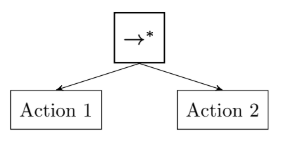
\includegraphics[width=0.4\textwidth]{images/SequenceCompositionWithMemory..png}
        \caption{Secuencia con memoria \protect\cite{colledanchise2018bt}}
        \label{fig:bt-secuencia-con-memoria}
    \end{figure}
    \begin{figure}[h]
        \centering
        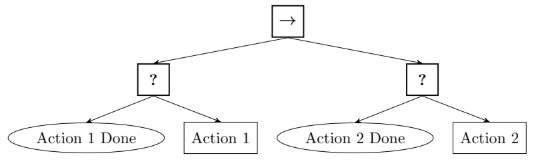
\includegraphics[width=0.8\textwidth]{images/SequenceCompositionWithMemoryEmulation.png}
        \caption{BT que emula la ejecución de una secuencia con memoria usando nodos sin memoria \protect\cite{colledanchise2018bt}}
        \label{fig:bt-secuencia-con-memoria-emulacion}
    \end{figure}

    \begin{itemize}
        \item Si la condición devuelve \textbf{SUCCESS} (porque la acción ya se realizó en un ciclo anterior), el nodo Fallback devuelve \textbf{SUCCESS} inmediatamente al padre sin volver a ejecutar la \textbf{Acción 1}. Esto permite que la secuencia pase directamente al siguiente hijo (\textbf{Acción 2}), emulando perfectamente el comportamiento de ``memoria''.\\
        \item Si la condición devuelve \textbf{FAILURE}, el Fallback procede a ejecutar la \textbf{Acción 1}.
    \end{itemize}

\end{itemize}

\subsubsection{Propiedades relevantes para sistemas robóticos}

Los BT presentan propiedades especialmente valiosas para el diseño de robots autónomos:

\begin{itemize}
    \item \textbf{Modularidad}: cada comportamiento puede construirse como un subárbol independiente.
    \item \textbf{Reactividad}: la evaluación por ticks permite decisiones continuas en lazo cerrado.
    \item \textbf{Legibilidad}: la estructura jerárquica facilita la comprensión del comportamiento, incluso en sistemas complejos.
    \item \textbf{Escalabilidad}: nuevos comportamientos pueden añadirse mediante composición sin modificar la arquitectura existente.
\end{itemize}

Estas características han contribuido a que los BT se conviertan en una arquitectura preferida tanto en investigación como en robótica industrial.

\subsubsection{Ejemplos conceptuales}

Para ilustrar su funcionamiento, pueden considerarse las siguientes estructuras básicas:

\paragraph{Sequence: Rutinas ordenadas}

\begin{verbatim}
Despertar → Cepillarse los dientes → Desayunar
\end{verbatim}

El nodo ejecuta cada acción en orden; si alguna falla, la secuencia completa se detiene y retorna fallo.

\paragraph{Selector: búsqueda de alternativas}

\begin{verbatim}
Buscar comida en la heladera → Pedir comida a domicilio → Resignarse
\end{verbatim}

El nodo prueba cada opción en orden; en cuanto una tiene éxito, el selector retorna éxito sin evaluar las restantes.

Estos patrones permiten expresar comportamientos complejos de manera clara, incremental y sin necesidad de programar grandes cantidades de transiciones explícitas entre estados, como ocurriría en una FSM.

% ===============================================================

\section{Implementación del motor BT}

El motor de árboles de comportamiento constituye uno de los pilares principales de este proyecto. Su función es proporcionar una estructura modular, jerárquica y extensible para la toma de decisiones, manteniéndose completamente independiente de la lógica de aplicación concreta. Esta desacoplación permite reutilizar el motor en distintos proyectos, modificar comportamientos sin alterar el núcleo del sistema e integrar nuevos sensores o actuadores sin comprometer la arquitectura general.

\subsubsection{Rol del BT dentro del sistema}

En la arquitectura del robot, el BT se sitúa como una capa lógica que organiza y ejecuta decisiones de manera ordenada. El motor opera exclusivamente sobre un contexto (\texttt{ctx}) que contiene el estado del sistema, y los nodos interactúan con funciones de bajo nivel a través de ese contexto. De esta forma, el BT no está vinculado a un conjunto predeterminado de acciones, sino que actúa como un orquestador general de comportamiento.

Esta separación entre el motor BT y la lógica de dominio permite:

\begin{itemize}
    \item reutilizar el BT en múltiples aplicaciones,
    \item mantener independencia respecto del hardware subyacente,
    \item facilitar modificaciones de comportamiento sin cambios estructurales,
    \item asegurar escalabilidad y limpieza conceptual a lo largo del proyecto.
\end{itemize}

\subsubsection{Restricciones y requisitos del entorno embebido}

La implementación del BT en Lua-RTOS se diseñó considerando las limitaciones propias del ESP32:

\begin{itemize}
    \item \textbf{memoria reducida}, que obliga a minimizar asignaciones y evitar estructuras complejas;
    \item \textbf{ejecución cooperativa}, donde ningún componente debe bloquear la CPU;
    \item \textbf{predictibilidad temporal}, esencial en sistemas reactivos;
    \item \textbf{robustez}, dado que el motor debe ejecutarse durante períodos prolongados sin fugas de memoria.
\end{itemize}

Estas restricciones guiaron varias decisiones de diseño del módulo.

\subsubsection{Estructura general del módulo \texttt{bt}}

El módulo \texttt{bt} implementa únicamente los componentes esenciales para componer comportamientos complejos:

\begin{itemize}
    \item \textbf{Nodos compositores}: \texttt{sequence} y \texttt{selector};
    \item \textbf{Nodos hoja}: \texttt{action} y \texttt{condition};
    \item \textbf{Decoradores}: \texttt{repeater}, \texttt{interrupt}, \texttt{interruptible};
    \item \textbf{Árbol principal}: construido mediante \texttt{bt.create\_tree}.
\end{itemize}

Cada nodo está implementado como una tabla Lua que define una interfaz estandarizada basada en dos métodos principales:

\begin{itemize}
    \item \textbf{tick(self, ctx)}: representa el ``latido'' del árbol. Es la señal que activa la lógica del nodo en cada ciclo. Al ser invocado, el nodo debe devolver inmediatamente uno de los tres estados de retorno: \texttt{SUCCESS}, \texttt{FAILURE} o \texttt{RUNNING}
    \item \textbf{reset(self)}: fundamental para la modularidad y reusabilidad del código. Este método restablece el estado interno del nodo e invoca de forma recursiva el reset de sus hijos. Esto asegura que los nodos vuelvan a su estado inicial tras un fallo o éxito, permitiendo que el árbol sea consistente en ejecuciones repetidas sin arrastrar residuos de ciclos anteriores
\end{itemize}

\subsubsection{Contexto y ejecución periódica}

El sistema de Árboles de Comportamiento opera sobre un contexto compartido, el cual actúa como una memoria de trabajo que contiene todas las variables y el estado necesarios para la toma de decisiones coordinada. El motor de ejecución se basa en un bucle principal no bloqueante que realiza llamadas periódicas al método \texttt{tree:run()}, el cual dispara una señal de activación denominada ``tick'' que se propaga de forma jerárquica desde el nodo raíz hacia las hojas. Este mecanismo de ``ticking'' continuo permite una ejecución en bucle cerrado (closed-loop), lo que garantiza que la solución sea altamente reactiva y capaz de abortar o reanudar tareas instantáneamente.\\

Para asegurar la estabilidad y el rendimiento, el objeto árbol incorpora los siguientes componentes técnicos:

\begin{itemize}
    \item \texttt{Contador de ticks interno}: registra de forma persistente el número de ciclos ejecutados desde el inicio o el último reinicio del sistema.
    \item \texttt{Gestión de memoria optimizada}: la implementación incluye un mecanismo explícito que invoca la función de Lua collectgarbage(``collect'') cada 500 ticks, lo que previene la fragmentación excesiva de la memoria y elimina pausas inesperadas por recolecciones automáticas agresivas.
    \item \texttt{Método de reinicio (reset)}: permite restablecer el árbol completo a su estado inicial, incluyendo la puesta a cero del contador de ticks y la invocación recursiva de la función reset en todos los nodos hijos para limpiar memorias internas y punteros de progresión
\end{itemize}

\subsubsection{Implementación de nodos en el motor BT}

El módulo \texttt{bt} desarrollado para este proyecto incluye una colección de nodos diseñada específicamente para funcionar de manera eficiente en Lua-RTOS sobre ESP32. A diferencia de motores BT más complejos, esta implementación prioriza simplicidad estructural, bajo consumo de memoria y ausencia de referencias circulares.

Los nodos disponibles son los siguientes:

\paragraph{1. Nodos hoja}

\begin{itemize}
    \item \textbf{\texttt{action(fn)}}: encapsula una acción potencialmente prolongada. El nodo ejecuta la función \texttt{fn(self, ctx)} y retorna \texttt{SUCCESS}, \texttt{FAILURE} o \texttt{RUNNING}. Permite conservar estado interno a través de campos como \texttt{self.started} o \texttt{self.counter}. Cada acción implementa opcionalmente un método \texttt{reset()} para reiniciar su estado.
   
    \item \textbf{\texttt{condition(fn)}}: evalúa una condición instantánea sobre el contexto. Retorna \texttt{SUCCESS} o \texttt{FAILURE}, sin estado persistente ni posibilidad de retornar \texttt{RUNNING}.
\end{itemize}

\paragraph{2. Nodos compositores}

\begin{itemize}
    \item \textbf{\texttt{sequence(children)}}: Nodo con memoria (utilizando un puntero interno \texttt{self.counter} para saltar directamente al hijo que quedó en estado de ejecución o al siguiente en la lista) que avanza de ``izquierda'' a ``derecha'' (del primer nodo hijo al último) y solo pasa al siguiente si el anterior devuelve \texttt{SUCCESS}. Si un hijo devuelve \texttt{RUNNING}, la secuencia se detiene y propaga ese estado. Si un hijo devuelve \texttt{FAILURE}, el nodo reinicia su puntero \texttt{self.counter} y ejecuta la función reset en todos sus hijos para garantizar modularidad en el próximo ciclo.
   
    \item \textbf{\texttt{selector(children)}}: Nodo con memoria que busca la primera alternativa exitosa, ejecutando a sus hijos en orden; si uno devuelve \texttt{SUCCESS}, el selector termina con éxito inmediatamente. Si un hijo devuelve \texttt{RUNNING}, la secuencia se detiene y propaga ese estado. Devuelve \texttt{FAILURE} únicamente si todos sus hijos fallan. Si los primeros hijos de un Selector fallan, el nodo recuerda esos fallos y no vuelve a intentarlos en los siguientes ticks, centrándose únicamente en la alternativa que devolvió RUNNING o en las restantes. Al igual que sequence, limpia su memoria interna y resetea a los hijos al finalizar con éxito o tras agotar las opciones.
\end{itemize}

La implementación de nodos Sequence y Selector con memoria en el módulo responde a necesidades tanto teóricas como de eficiencia técnica. En este caso específico, su uso es necesario por las siguientes razones fundamentales:

\begin{itemize}
    \item \textbf{Evitar la re-ejecución innecesaria de tareas}: en un árbol sin memoria, cada ``tick'' reinicia la evaluación desde el primer hijo de la izquierda. Sin embargo, en muchos escenarios de robótica, una vez que un sub-objetivo se ha alcanzado, no es necesario volver a comprobarlo en cada ciclo si el entorno es predecible. Este es el escenarios particular de nuestro robot, donde las secuencias son controladas y predecibles.
   
    \item \textbf{Reducción del costo computacional}: al mantener el puntero interno \texttt{self.counter} hacia el hijo que devolvió \texttt{RUNNING}, el sistema no malgasta recursos re-evaluando ramas del árbol que ya terminaron su labor. Esto permite que el árbol funcione de manera más fluida en sistemas con recursos limitados.
   
    \item \textbf{Continuidad de acciones en estado RUNNING}: técnicamente, en la implementación del módulo, cuando un hijo devuelve \texttt{RUNNING}, el nodo padre debe devolver lo mismo inmediatamente para ceder el control. Por lo tanto, la memoria es vital aquí para que, en el siguiente tick, el árbol sepa exactamente dónde retomar el trabajo. Sin memoria, el ``tick'' volvería al primer hijo, lo que podría interrumpir la acción que estaba en curso o causar comportamientos erráticos.
\end{itemize}

Es importante recordar que, esta memoria no es permanente: se limpia automáticamente en cuanto el nodo completo termina con éxito o falla, asegurando que el comportamiento pueda reiniciarse correctamente en el futuro

\paragraph{3. Nodos decoradores}

\begin{itemize}
    \item \textbf{\texttt{repeater(child, n)}}: repite la ejecución del nodo hijo \texttt{n} veces, o indefinidamente si \texttt{$n = -1$}. Entre repeticiones invoca \texttt{reset()} en el hijo para garantizar consistencia.
   
    \begin{itemize}
        \item \texttt{Comportamiento del Tick}: cuando recibe un tick, ejecuta a su hijo. Si el hijo devuelve \texttt{RUNNING}, el repetidor propaga \texttt{RUNNING} hacia arriba. Si el hijo devuelve \texttt{SUCCESS} o \texttt{FAILURE}, el repetidor incrementa su contador interno, resetea al hijo para que pueda ejecutarse de nuevo en el siguiente ciclo y devuelve \texttt{RUNNING} para indicar que el proceso de repetición continúa.
       
        \item \texttt{Condición de Éxito}: solo devuelve \texttt{SUCCESS} cuando se ha alcanzado el límite de repeticiones definido \texttt{(max\_repeats)}. Si se configura con \texttt{$n = -1$}, se convierte en un bucle infinito.

        \item \texttt{Memoria}: implementa memoria mediante la variable current\_count, la cual rastrea cuántas iteraciones se han completado a través de múltiples ticks. Esta memoria se limpia mediante la función \textbf{\texttt{reset()}} o automáticamente al completar todas las repeticiones.
    \end{itemize}
   
    \item \textbf{\texttt{interrupt(condition, child)}}: representa un evento prioritario. Evalúa una condición externa y, si se cumple, ejecuta el nodo hijo de la interrupción. Retorna el estado del hijo y posee su propio mecanismo de \texttt{reset()}.

    \begin{itemize}
        \item \texttt{Mecanismo Clave}: posee un método único llamado \textbf{\texttt{should\_interrupt(ctx)}}, que evalúa una función de condición proporcionada por el usuario. Esto permite que otros nodos consulten si se debe disparar la interrupción antes de procesar el flujo normal del árbol
   
        \item \texttt{Comportamiento del Tick}: si es activado, simplemente ejecuta a su hijo y devuelve su estado. Si no tiene un hijo asignado, devuelve \texttt{SUCCESS} por defecto al dispararse la condición.
       
        \item \texttt{Condición de Éxito}: devuelve \texttt{SUCCESS} cuando la condición se activa y su hijo devuelve \texttt{SUCCESS}. Si no tiene hijo asignado y la condición se activa, devuelve \texttt{SUCCESS} directamente.

        \item \texttt{Memoria}: su función es evaluativa e instantánea, aunque su hijo puede tener su propia lógica interna.
    \end{itemize}
   
    \item \textbf{\texttt{interruptible(child, interrupts, reset\_on\_interrupt)}}: funciona como un decorador especializado que envuelve a un nodo hijo principal con una lista de nodos \texttt{interrupts} para gestionar la preemción explícita.\\
    En cada ciclo de ejecución, el nodo realiza una verificación de seguridad tanto antes como después de ejecutar al hijo, consultando si algún componente de la lista de interrupciones activa su señal mediante el método \textbf{\texttt{should\_interrupt(ctx)}}. Si se detecta una interrupción válida y la propiedad \textbf{\texttt{reset\_on\_interrupt}} está habilitada (la cual es true por defecto), el nodo invoca inmediatamente la función reset del hijo para limpiar cualquier estado residual o contador interno antes de proceder con la lógica de la interrupción. Este mecanismo de doble chequeo es fundamental para la reactividad del sistema, ya que permite invalidar instantáneamente el progreso de un hijo que devuelva el estado \texttt{RUNNING} si las condiciones críticas del entorno cambian en ese mismo instante. \\
    Finalmente, para asegurar la modularidad y la reusabilidad del código, el método reset de este componente se encarga de reiniciar recursivamente tanto al nodo hijo como a todos los nodos dentro de la lista de interrupciones. \\
    Gracias a este diseño, el árbol de comportamiento puede abortar tareas activas y responder a eventos de mayor prioridad de forma inmediata, cumpliendo con la premisa de ejecución en bucle cerrado y preemción reactiva
\end{itemize}

\paragraph{4. Nodo raíz del árbol}

\begin{itemize}
    \item \textbf{\texttt{create\_tree(root)}}: construye la estructura del árbol a partir de un nodo raíz. El árbol mantiene un contador interno de ticks, ejecuta \texttt{root:tick(ctx)} en cada invocación de \texttt{run()} y dispara manualmente el recolector de basura cada 500 ticks para evitar acumulación de fragmentación.
\end{itemize}

Este conjunto de nodos conforma un motor BT completo, compacto y adecuado para sistemas embebidos, manteniendo compatibilidad con las estructuras clásicas de Behavior Trees y añadiendo mecanismos de interrupción apropiados para entornos reactivos.


\subsubsection{Mecanismo de interrupciones}

El módulo incorpora un sistema de interrupciones diseñado para actuar como una capa de seguridad y prioridad sobre cualquier tarea en curso, apoyándose en los nodos especializados  \texttt{interrupt} e  \texttt{interruptible}. En lugar de mezclar la lógica de emergencia con las actividades principales, este mecanismo supervisa constantemente un conjunto de condiciones críticas en cada ciclo de ejecución. La clave de su efectividad reside en que realiza estas comprobaciones en dos momentos fundamentales de cada ``tick'': justo antes de iniciar una tarea y nuevamente después, lo que garantiza que el sistema reaccione de inmediato ante cambios en el entorno, incluso si una acción prolongada todavía se encuentra en ejecución. \\
Si se detecta que una condición de alta prioridad se ha activado, el sistema tiene la capacidad de abortar y reiniciar limpiamente el comportamiento que estaba activo, eliminando cualquier residuo del estado anterior para asegurar la consistencia en el futuro. Este diseño permite modelar eventos inesperados de forma lógica y organizada, manteniendo la estructura del árbol intacta y logrando una separación clara entre los comportamientos principales y las reacciones de emergencia necesarias para la seguridad del agente

Este mecanismo permite modelar eventos asincrónicos desde el punto de vista lógico, manteniendo un diseño limpio y sin mezclas entre comportamientos principales y reacciones de emergencia.

\subsubsection{Gestión de memoria y diseño sin referencias circulares}

El módulo evita deliberadamente:

\begin{itemize}
    \item referencias a nodos padre,
    \item registros globales,
    \item estructuras de introspección o depuración complejas.
\end{itemize}

Al no generar ciclos de referencia, Lua puede liberar memoria con seguridad. El disparo explícito del recolector cada 500 ticks permite controlar la fragmentación y prevenir pausas largas.

\subsubsection{Integración con módulos externos}

El BT no interactúa directamente con hardware ni sensores. Todas las funciones son encapsuladas en el contexto (\texttt{ctx}) y expuestas mediante APIs en Lua o C. De esta forma:

\begin{itemize}
    \item el BT decide \emph{qué} se debe hacer,
    \item los módulos externos implementan \emph{cómo} hacerlo.
\end{itemize}

Este diseño mantiene la portabilidad y evita dependencia directa entre el motor BT y los subsistemas específicos del robot.

\subsubsection{Extensibilidad}

La estructura del motor permite integrar nuevos módulos, acciones y comportamientos sin modificar el núcleo del sistema. Cualquier nueva lógica de decisión puede modelarse mediante combinaciones de los nodos existentes, preservando la sencillez del motor central.

Esta independencia funcional convierte al BT en un componente reutilizable, adaptable y adecuado para múltiples entornos educativos y robóticos.


\chapter{Creación del juego (reglas, dinámica y objetivos pedagógicos)}

El juego desarrollado propone una actividad didáctica en la que un robot móvil recorre un circuito establecido sobre un tatami, interpretando señales visuales y verificando el orden correcto de una serie de elementos colocados por los estudiantes. El diseño combina exploración autónoma, reconocimiento visual y retroalimentación inmediata, permitiendo que los niños participen activamente en la construcción del recorrido y la validación de la secuencia propuesta.

\section{Diseño y dinámica del juego}

El escenario de juego está compuesto por una superficie de tatami sobre la cual se traza una línea guía que el robot debe seguir de manera autónoma. A lo largo del circuito se ubican distintas “estaciones visuales”, formadas por marcos laterales donde los estudiantes insertan imágenes, ilustraciones o símbolos. Cada marco contiene además un código QR con un identificador numérico (\emph{id} = 1, 2, 3, ...), el cual representa la posición correcta que debería ocupar ese elemento dentro de la secuencia.

Además, en algunos tramos del tatami se adhieren pequeños adhesivos. Estas marcas cumplen la función de activar un evento dentro de la partida: cuando el robot las detecta, debe detenerse y ejecutar una verificación sobre la estación visual correspondiente.

\subsection{Reglas del juego}

Las reglas del juego se describen a continuación:

\begin{itemize}
    \item \textbf{Inicio}: el robot se coloca en una casilla o pieza de inicio. Permanece en estado de espera activo hasta recibir la señal de comienzo, la cual consiste en mostrarle un indicador de color verde que contiene una etiqueta específica (QR) dentro. Una vez detectada esta señal, inicia el recorrido.
    
    \item \textbf{Seguimiento de línea}: el robot avanza siguiendo la línea trazada sobre el tatami. Esta línea define el trayecto general y garantiza que el robot atraviese todas las estaciones visuales.
    
    \item \textbf{Detección de pegotín rojo}: cuando el robot detecta un indicador de color rojo que contiene una etiqueta específica (QR) en el camino, debe detenerse y comenzar a girar sobre su eje para orientarse hacia los marcos laterales ubicados a ambos costados de la línea.
    
    \item \textbf{Lectura del código QR}: durante la rotación, el robot identifica el código QR correspondiente a la estación. Cada QR posee un identificador numérico que representa la posición correcta de esa imagen en la secuencia.
    
    \item \textbf{Verificación de orden}: los estudiantes y docentes colocan previamente las imágenes en los marcos. La misión consiste en ordenar correctamente dicha secuencia. El robot compara el \emph{id} leído con el orden esperado y:
    \begin{itemize}
        \item enciende una luz \textbf{verde} si el elemento es correcto,
        \item enciende una luz \textbf{roja} si el elemento está fuera de lugar.
    \end{itemize}
    
    \item \textbf{Retorno al recorrido}: tras la verificación, el robot gira nuevamente hasta alinearse con la línea de guía, retoma el seguimiento y continúa hacia la siguiente estación.
    
    \item \textbf{Final del recorrido}: al alcanzar la pieza final del circuito, el robot presenta un resultado global:
    \begin{itemize}
        \item Si toda la secuencia es correcta, activa un patrón de luces \textbf{verdes} y realiza un giro de celebración.
        \item Si existen errores, ilumina un patrón combinado que refleja el estado de cada estación evaluada. Se divide el anillo LED en la misma cantidad de segmentos que estaciones visitadas. Luego, las estaciones que se encuentren en orden correcto mostrarán un color \textbf{verde} y las estaciones que no se encuentren en el orden incorrecto mostrarán un color \textbf{rojo}.
    \end{itemize}
    
    \item \textbf{Estado de espera}: una vez finalizada la verificación global, el robot entra nuevamente en modo de espera, preparado para una nueva partida cuando se le muestre otra tarjeta de inicio.
\end{itemize}

\subsection{Modo pausa y modo reset}

Además del comportamiento principal del recorrido, el robot incorpora dos modos especiales de operación que permiten al docente intervenir en cualquier momento del juego sin perder el hilo de la actividad: \emph{pausa} y \emph{reset}.

\begin{itemize}
    \item \textbf{Modo pausa}: cuando el robot es levantado del tatami, detecta esta condición y entra automáticamente en un estado de pausa. En este modo deja de avanzar, detiene cualquier acción en curso y conserva íntegramente su estado interno (secuencia evaluada, posiciones visitadas y resultado parcial). Este modo resulta especialmente útil para que la maestra pueda detener la actividad, explicar un concepto, reorganizar una estación o asistir a un estudiante sin que el robot continúe moviéndose.
    
    \item \textbf{Reanudación del juego}: al volver a apoyar el robot en el piso, éste queda a la espera de una señal externa. Si recibe la señal de \textbf{continuar}, retoma el recorrido exactamente en la etapa en la que lo había dejado antes de ser levantado, sin perder los datos de las estaciones ya evaluadas.
    
    \item \textbf{Modo reset}: si en lugar de la señal de continuar el robot recibe una señal de \textbf{reinicio}, borra su estado interno, reinicia contadores, vacía el registro de estaciones correctas/incorrectas y vuelve a su comportamiento inicial, como si la partida comenzara desde cero. Este modo permite reiniciar el juego de forma rápida y ordenada cuando se desea realizar una nueva prueba sin tener que reubicar manualmente al robot en la pieza de inicio.
\end{itemize}


La inclusión de los modos \emph{pausa}, \emph{continuar} y \emph{reset} aporta beneficios tanto operativos como pedagógicos:

\begin{itemize}
    \item \textbf{Seguridad y control del entorno}: la maestra puede detener el robot inmediatamente ante cualquier situación (un niño cruza la trayectoria, se detecta un obstáculo inesperado, surge una pregunta importante, etc.).
    
    \item \textbf{Continuidad pedagógica}: el modo pausa permite explicar conceptos en el momento exacto en que surgen, sin perder el contexto del juego.
    
    \item \textbf{Gestión eficiente del tiempo de clase}: el modo continuar evita repetir partes del juego innecesariamente, evitando posible frustraciones o aburrimiento por parte de los estudiantes.
    
    \item \textbf{Flexibilidad en la dinámica del juego}: el modo reset habilita comenzar una nueva partida de forma instantánea, facilitando la repetición de actividades, la comparación de resultados o la experimentación con variantes del recorrido.
    
    \item \textbf{Comprensión profunda del proceso}: estos modos introducen a los estudiantes en nociones básicas de estados del sistema (pausa, ejecución, reinicio), similares a las empleadas en sistemas reales de robótica y programación.
\end{itemize}

\subsection{Implementación del juego utilizando BT}

\begin{figure}[!htbp]
    \centering
    \makebox[\textwidth][c]{%
        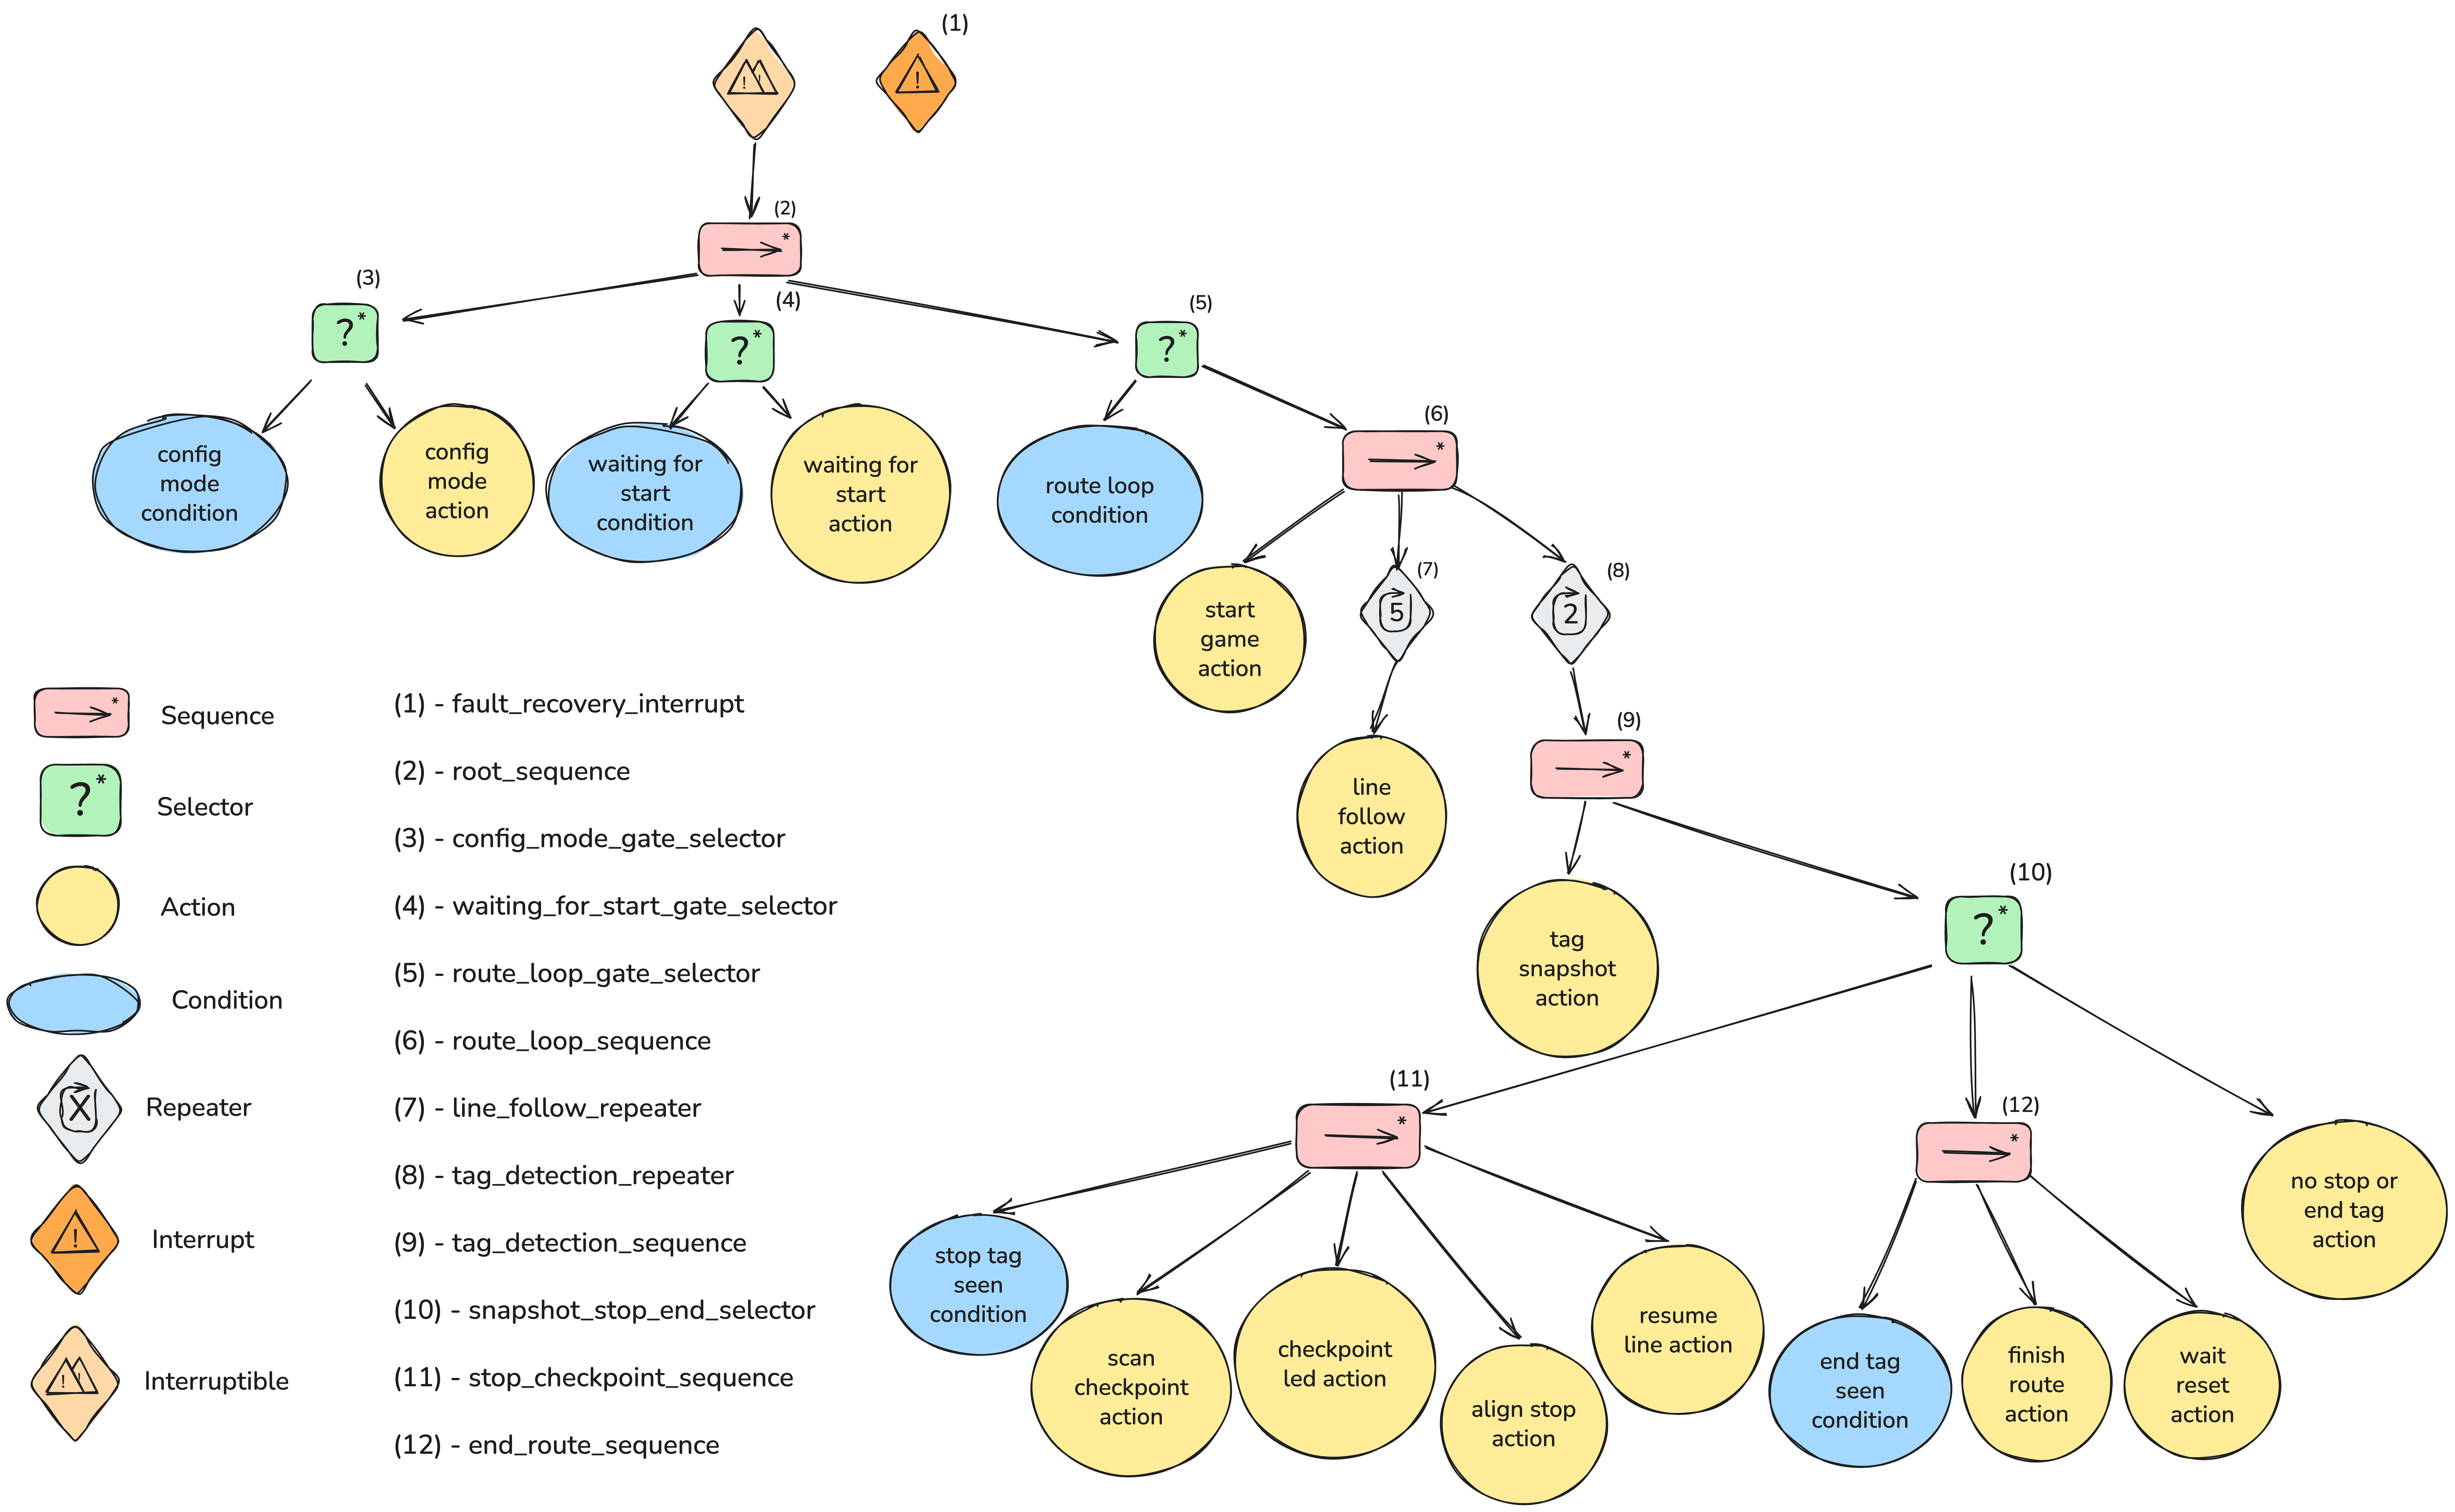
\includegraphics[width=1.3\textwidth]{images/BTRobotito.png}
    }
    \caption{Árbol de comportamiento implementado en Robotito.}
    \label{fig:bt_robotito}
\end{figure}

La lógica de control del juego fue implementada utilizando Árboles de Comportamiento (Behavior Trees, BT), debido a las ventajas que esta arquitectura ofrece en términos de modularidad, reactividad y claridad estructural. A diferencia de una Máquina de Estados Finitos (FSM), donde las transiciones entre estados pueden crecer exponencialmente a medida que aumenta la complejidad del sistema, los BT permiten encapsular comportamientos independientes en nodos reutilizables y organizarlos jerárquicamente.

En el contexto de Robotito, esta decisión permitió integrar de forma ordenada el seguimiento de línea, la detección de tags visuales, las rutinas de checkpoint y los mecanismos de recuperación ante errores. Además, la estructura jerárquica del árbol facilita la comprensión del flujo lógico del robot, lo cual resulta especialmente valioso desde el punto de vista pedagógico, ya que los estudiantes pueden visualizar claramente cómo el robot toma decisiones y responde al entorno.

El árbol se evalúa de forma periódica mediante \textit{ticks} ejecutados por el motor BT desarrollado en el proyecto. En cada \textit{tick}, los nodos son recorridos de arriba hacia abajo siguiendo las reglas de evaluación propias de cada tipo de nodo (\textit{Sequence}, \textit{Selector}, \textit{Repeater}, \textit{Condition} y \textit{Action}). Esta evaluación continua permite que el robot reaccione dinámicamente a cambios del entorno sin necesidad de reiniciar la ejecución completa del comportamiento.

La arquitectura final del árbol implementado se organiza en múltiples niveles jerárquicos, descritos a continuación.

\subsubsection{Nivel 0: Raíz de Seguridad (Envoltorio General)}

El nivel superior del árbol corresponde a un nodo de tipo \textit{interruptible}, cuya función principal es actuar como envoltorio de seguridad del sistema completo.

Este nodo posee asociada la interrupción:

\begin{itemize}
    \item \texttt{fault\_recovery\_interrupt}
\end{itemize}

La interrupción monitorea permanentemente condiciones críticas del robot durante toda la ejecución del juego. Entre los eventos supervisados se encuentran:

\begin{itemize}
    \item \texttt{proximity\_lost}: pérdida de referencia de proximidad o condiciones inseguras de navegación.
    \item \texttt{arrow\_fault}: inconsistencias en la detección o interpretación de flechas/direcciones.
    \item \texttt{checkpoint\_scan\_error}: fallo en el escaneo o validación de checkpoints.
\end{itemize}

Cuando alguna de estas condiciones ocurre, el árbol puede abortar inmediatamente la ejecución del comportamiento actual y derivar hacia rutinas de recuperación o detención segura. Este mecanismo proporciona una capa de robustez reactiva que evita bloqueos o comportamientos peligrosos.

El hijo principal de este nodo es:

\begin{itemize}
    \item \texttt{root\_sequence}
\end{itemize}

De esta forma, toda la lógica operacional queda encapsulada dentro de una estructura supervisada por mecanismos de seguridad globales.

\subsubsection{Nivel 1: Secuencia de Ciclo de Vida}

El nodo \texttt{root\_sequence} corresponde a una secuencia principal de tipo \textit{sequence}.

Su responsabilidad es gestionar el ciclo de vida completo del robot dentro del juego, organizando las diferentes etapas de funcionamiento:

\begin{enumerate}
    \item Configuración inicial.
    \item Espera de inicio.
    \item Ejecución del recorrido.
    \item Finalización y espera de reinicio.
\end{enumerate}

La secuencia garantiza que cada fase se complete exitosamente antes de permitir el avance hacia la siguiente. Esto resulta especialmente importante para evitar que el robot inicie la misión sin haber completado correctamente la inicialización del hardware o sin haber detectado el evento de comienzo del juego.

La lógica de transición entre fases se implementa mediante selectores denominados ``puertas'' (\textit{gate selectors}), los cuales habilitan o bloquean dinámicamente el avance según el estado interno del sistema.

\subsubsection{Nivel 2: Puertas de Fase (Gate Selectors)}

En este nivel se encuentran tres nodos de tipo \textit{selector}, cada uno asociado a una etapa específica del funcionamiento del robot:

\paragraph{\texttt{config\_mode\_gate\_selector}}

Determina si es necesario ejecutar la fase de configuración e inicialización del hardware.

Esta puerta permite reutilizar el árbol tanto en arranques completos como en reinicios parciales, evitando reinicializaciones innecesarias cuando el sistema ya se encuentra configurado.

\paragraph{\texttt{waiting\_for\_start\_gate\_selector}}

Gestiona el estado de espera previo al inicio de la actividad.

Durante esta etapa el robot permanece en modo Standby hasta detectar el tag o condición visual que habilita el comienzo del juego. Esto permite que el docente o los estudiantes preparen el circuito antes de iniciar la ejecución.

\paragraph{\texttt{route\_loop\_gate\_selector}}

Habilita el acceso al ciclo operativo principal de la misión.

Una vez atravesadas las etapas anteriores, esta puerta permite ejecutar el recorrido autónomo del robot sobre el circuito.

\subsubsection{Nivel 3: Lógica Interna de las Puertas}

Cada selector implementa internamente una lógica basada en condiciones y acciones.

\paragraph{Hijos de \texttt{config\_mode\_gate\_selector}}

\begin{itemize}
    \item \texttt{config\_mode\_condition}
    \item \texttt{config\_mode\_action}
\end{itemize}

La condición verifica si el hardware ya fue inicializado correctamente. En caso contrario, se ejecuta la acción correspondiente, encargada de:

\begin{itemize}
    \item Inicializar sensores.
    \item Configurar la cámara HuskyLens.
    \item Validar la comunicación I2C.
    \item Reiniciar variables globales.
    \item Preparar estructuras internas del BT.
\end{itemize}

\paragraph{Hijos de \texttt{waiting\_for\_start\_gate\_selector}}

\begin{itemize}
    \item \texttt{waiting\_for\_start\_condition}
    \item \texttt{waiting\_for\_start\_action}
\end{itemize}

La condición verifica si el evento de inicio ya fue detectado. Mientras esto no ocurra, la acción mantiene al robot en estado de espera.

Durante este modo pueden ejecutarse mecanismos de feedback visual, como LEDs o señales luminosas, indicando que el robot se encuentra listo para comenzar.

\paragraph{Hijos de \texttt{route\_loop\_gate\_selector}}

\begin{itemize}
    \item \texttt{route\_loop\_condition}
    \item \texttt{route\_loop\_sequence}
\end{itemize}

La condición valida que el juego esté efectivamente habilitado para ejecutarse. Si esto se cumple, se ingresa a la secuencia principal de navegación y procesamiento de eventos del recorrido.

\subsubsection{Nivel 4: Bucle Operativo de la Misión (\texttt{route\_loop\_sequence})}

El nodo \texttt{route\_loop\_sequence} es una secuencia principal de tipo \textit{sequence} encargada de ejecutar el comportamiento operativo del robot durante la misión.

Sus hijos son:

\paragraph{\texttt{start\_game\_action}}

Activa la flag interna \texttt{is\_running}, habilitando el funcionamiento completo del sistema y permitiendo que las interrupciones críticas comiencen a actuar sobre el árbol.

Esta acción marca formalmente el inicio de la misión.

\paragraph{\texttt{line\_follow\_repeater}}

Nodo repetidor encargado de ejecutar el comportamiento de seguimiento de línea una cantidad N de veces.

El uso de un repetidor desacopla la lógica de navegación continua del resto de los comportamientos del árbol y permite ajustar dinámicamente la duración o persistencia del seguimiento.

\paragraph{\texttt{tag\_detection\_repeater}}

Nodo repetidor encargado de ejecutar la lógica de detección de tags visuales una cantidad M de veces.

Esto permite que el robot inspeccione continuamente el entorno en busca de checkpoints, marcas STOP o tags END sin interrumpir permanentemente el movimiento general.

\subsubsection{Nivel 5: Hijos de los Repetidores}

\paragraph{\texttt{line\_follow\_repeater}}

Contiene como hijo único:

\begin{itemize}
    \item \texttt{line\_follow\_action}
\end{itemize}

Esta acción implementa el algoritmo de seguimiento de línea utilizando la información proporcionada por HuskyLens.

El comportamiento ajusta dinámicamente la velocidad de los motores para mantener el robot alineado con la trayectoria marcada en el tatami. Además, puede incluir:

\begin{itemize}
    \item Correcciones proporcionales.
    \item Recentrado de trayectoria.
    \item Reducción de velocidad en curvas.
    \item Estabilización ante ruido visual.
\end{itemize}

\paragraph{\texttt{tag\_detection\_repeater}}

Contiene como hijo:

\begin{itemize}
    \item \texttt{tag\_detection\_sequence}
\end{itemize}

Esta secuencia concentra toda la lógica asociada al procesamiento visual de etiquetas y eventos del entorno.

\subsubsection{Nivel 6: Procesamiento de Visión (\texttt{tag\_detection\_sequence})}

El nodo \texttt{tag\_detection\_sequence} es una secuencia encargada de procesar la información visual capturada por HuskyLens.

Sus hijos son:

\paragraph{\texttt{tag\_snapshot\_action}}

Captura una ``instantánea'' del estado visual actual del entorno.

En lugar de consultar continuamente la cámara durante toda la evaluación del árbol, esta acción genera una fotografía lógica del conjunto de tags visibles en ese instante y la almacena en el contexto del BT.

Este enfoque presenta varias ventajas:

\begin{itemize}
    \item Reduce lecturas redundantes.
    \item Mantiene coherencia temporal durante la evaluación.
    \item Evita inconsistencias causadas por cambios rápidos en la imagen.
    \item Simplifica la toma de decisiones en niveles posteriores.
\end{itemize}

\paragraph{\texttt{snapshot\_stop\_end\_selector}}

Evalúa el contenido de la captura y decide cuál rama del árbol ejecutar a continuación.

\subsubsection{Nivel 7: Selector de Rama de Estación (\texttt{snapshot\_stop\_end\_selector})}

Este nodo es un \textit{selector} responsable de decidir qué comportamiento ejecutar según los tags detectados en la captura visual.

Sus hijos son:

\paragraph{\texttt{stop\_checkpoint\_sequence}}

Rama especializada para el procesamiento de checkpoints o estaciones STOP.

\paragraph{\texttt{end\_route\_sequence}}

Rama destinada a la detección del final del recorrido.

\paragraph{\texttt{no\_stop\_or\_end\_tag\_action}}

Acción por defecto ejecutada cuando no se detecta ningún tag relevante.

Generalmente esta acción retorna éxito inmediato o simplemente mantiene el flujo operativo normal del robot, permitiendo continuar el seguimiento de línea sin interrupciones.

\subsubsection{Nivel 8: Secuencias de Acción Específicas}

\paragraph{Rama \texttt{stop\_checkpoint\_sequence}}

Corresponde a una secuencia de acciones ejecutadas cuando el robot detecta un tag STOP.

Sus hijos son:

\begin{itemize}
    \item \texttt{stop\_tag\_seen\_condition}
    \item \texttt{scan\_checkpoint\_action}
    \item \texttt{checkpoint\_led\_action}
    \item \texttt{align\_stop\_action}
    \item \texttt{resume\_line\_action}
\end{itemize}

\paragraph{\texttt{stop\_tag\_seen\_condition}}

Verifica si efectivamente existe un tag STOP válido en la captura actual.

\paragraph{\texttt{scan\_checkpoint\_action}}

Ejecuta un movimiento de búsqueda o escaneo.

Normalmente implica pequeñas rotaciones o ajustes de orientación para mejorar la visibilidad de los elementos del checkpoint y permitir una detección más robusta.

\paragraph{\texttt{checkpoint\_led\_action}}

Realiza la validación del checkpoint y proporciona retroalimentación visual mediante LEDs.

Este feedback inmediato resulta importante desde el punto de vista pedagógico, ya que permite a los estudiantes observar claramente cuándo una estación fue reconocida correctamente.

\paragraph{\texttt{align\_stop\_action}}

Alinea el robot respecto al tag detectado.

La alineación mejora la estabilidad del sistema antes de continuar el recorrido y reduce errores acumulativos de orientación.

\paragraph{\texttt{resume\_line\_action}}

Realiza una fase de estabilización para reincorporarse correctamente a la línea guía luego de abandonar temporalmente el recorrido durante el proceso de checkpoint.

\paragraph{Rama \texttt{end\_route\_sequence}}

Esta secuencia se ejecuta cuando se detecta el tag de finalización del recorrido.

Sus hijos son:

\begin{itemize}
    \item \texttt{end\_tag\_seen\_condition}
    \item \texttt{finish\_route\_action}
    \item \texttt{wait\_reset\_action}
\end{itemize}

\paragraph{\texttt{end\_tag\_seen\_condition}}

Verifica la presencia válida de un tag END.

\paragraph{\texttt{finish\_route\_action}}

Finaliza formalmente la misión.

Esta acción incluye:

\begin{itemize}
    \item Detención del robot.
    \item Cálculo de puntaje o resultado final.
    \item Verificación de checkpoints completados.
    \item Retroalimentación visual.
    \item Secuencias de celebración mediante LEDs o movimientos.
\end{itemize}

\paragraph{\texttt{wait\_reset\_action}}

Mantiene el robot en estado de espera hasta recibir un comando de reinicio.

Esto evita reinicios accidentales y permite reutilizar el circuito múltiples veces sin reinicializar completamente el sistema.

\subsubsection{Consideraciones generales sobre el diseño del árbol}

La arquitectura implementada presenta varias ventajas importantes:

\begin{itemize}
    \item Modularidad: cada comportamiento se encuentra encapsulado en nodos independientes.
    \item Reutilización: acciones y condiciones pueden reutilizarse en futuros proyectos.
    \item Reactividad: las interrupciones permiten responder inmediatamente a eventos críticos.
    \item Escalabilidad: nuevas ramas o comportamientos pueden añadirse sin modificar la estructura general.
    \item Legibilidad: la jerarquía del árbol facilita el análisis y depuración del sistema.
    \item Valor pedagógico: el flujo lógico resulta visualmente interpretable para estudiantes y docentes.
\end{itemize}

Además, el uso de BT permitió separar claramente la percepción visual, la toma de decisiones y el control cinemático del robot, siguiendo principios modernos de arquitectura robótica.

\subsection{Dinámica interactiva}

La dinámica del juego involucra activamente a los estudiantes:

\begin{enumerate}
    \item Los niños eligen imágenes o dibujos relacionados con una temática propuesta (animales, letras, números, emociones, etc.).
    \item Insertan cada imagen en un marco con QR y deciden su ubicación en el circuito.
    \item Se inicia la partida y el robot recorre el mapa verificando la secuencia.
    \item El sistema proporciona retroalimentación inmediata mediante señales lumínicas.
    \item Los estudiantes interpretan los resultados, discuten errores y reorganizan la secuencia si es necesario.
\end{enumerate}

Este proceso genera un ciclo de juego–retroalimentación–corrección altamente motivador.

\subsection{Objetivos pedagógicos}

El juego está diseñado para cumplir objetivos educativos específicos:

\begin{itemize}
    \item \textbf{Ordenamiento y secuenciación}: los estudiantes deben organizar elementos siguiendo un criterio lógico (numérico, temático, temporal, narrativo).
    \item \textbf{Reconocimiento visual y espaciamiento}: comprender la relación entre la ubicación física de las imágenes y su identificador digital (QR).
    \item \textbf{Pensamiento computacional}: relacionar la secuencia física con el procesamiento interno del robot.
    \item \textbf{Resolución de problemas}: interpretar la retroalimentación del robot, identificar fallos en la secuencia y corregirlos.
    \item \textbf{Participación activa y colaborativa}: las docentes y estudiantes construyen juntos el escenario de juego y analizan los resultados.
\end{itemize}

\subsection{Variedad y adaptabilidad de la actividad}

El juego permite múltiples variantes educativas:

\begin{itemize}
    \item Cambiar la temática de las imágenes (historias, animales, señales, letras).
    \item Variar la dificultad aumentando la cantidad de estaciones.
    \item Plantear secuencias crecientes, decrecientes o basadas en categorías.
    \item Introducir estaciones sin pegotín rojo.
\end{itemize}

En conjunto, el diseño del juego sirve como puente entre el razonamiento lógico, la robótica educativa y la interacción con un sistema autónomo de manera accesible y motivadora.

\chapter{Configurador web para la preparación de secuencias de Robotito}

\section{Introducción y requerimientos funcionales}

Dentro de la plataforma Robotito se identificó la necesidad de contar con una herramienta que permitiera preparar recorridos y configuraciones de uso sin modificar directamente el firmware del robot ni depender de entornos de programación complejos. Con este objetivo, se desarrolló un configurador web orientado a facilitar la carga, organización y envío de secuencias de tags físicos.

El configurador cumple una función de apoyo dentro del sistema general. Su propósito principal es permitir que el usuario registre tags, defina relaciones de equivalencia entre ellos, construya secuencias de recorrido, cargue actividades predefinidas y transfiera dicha información al robot para su posterior ejecución en la actividad didáctica.

Desde el punto de vista funcional, la herramienta debe cumplir los siguientes requerimientos:

\begin{itemize}
    \item \textbf{RF-01: Lectura de tags físicos.} Permitir la detección de tags mediante la cámara del dispositivo.
    
    \item \textbf{RF-02: Gestión del catálogo de tags.} Registrar tags, asignarles nombres o alias lógicos y organizarlos para su uso en secuencias.
    
    \item \textbf{RF-03: Definición de intercambiabilidad.} Permitir que distintos tags físicos puedan ser tratados como equivalentes cuando representan una misma función dentro de la actividad.
    
    \item \textbf{RF-04: Validación de secuencias.} Verificar que las rutas definidas por el usuario respeten las restricciones básicas del sistema antes de ser enviadas al robot.
    
    \item \textbf{RF-05: Transferencia de configuración.} Enviar al robot las secuencias preparadas para que puedan ser utilizadas durante la actividad didáctica.

    \item \textbf{RF-06: Biblioteca de actividades.} Permitir la carga de actividades predefinidas que incluyan secuencias, grupos de tags, estaciones y relaciones de intercambiabilidad.
\end{itemize}

\section{Rol del configurador dentro del sistema}

El configurador web actúa como una capa intermedia entre el usuario y el robot. Su objetivo no es reemplazar la lógica embebida del sistema, sino facilitar la preparación de las condiciones iniciales de trabajo.

En términos funcionales, el flujo de uso del configurador es el siguiente:

\begin{enumerate}
    \item El usuario selecciona una actividad predefinida o inicia una configuración manual.
    \item El sistema incorpora los tags, grupos, estaciones y secuencias asociados a la actividad seleccionada.
    \item El usuario registra o ajusta los tags físicos disponibles.
    \item El usuario define, si corresponde, qué tags pueden considerarse equivalentes.
    \item Se construyen o modifican una o más secuencias de recorrido.
    \item El configurador valida que las secuencias sean consistentes.
    \item La configuración se transfiere al robot.
\end{enumerate}

De esta manera, el configurador reduce la intervención técnica necesaria durante la actividad y permite que la preparación del recorrido se realice desde una interfaz accesible para el usuario.

\section{Lectura de tags desde la cámara}

La detección de tags se realiza utilizando la cámara del dispositivo desde el navegador. El usuario presenta un marcador físico frente a la cámara y, una vez reconocido, el sistema lo incorpora al catálogo de tags disponibles.

Para evitar registros incorrectos causados por movimientos, desenfoque, variaciones de iluminación u oclusiones parciales, el sistema exige que un mismo marcador sea detectado de forma estable antes de confirmar su registro. Además, si aparecen múltiples tags simultáneamente, el sistema evita registrar automáticamente la lectura para prevenir ambigüedades.

Esta funcionalidad permite que el usuario trabaje directamente con los elementos físicos del entorno, vinculando cada marcador real con su representación dentro del configurador.

\begin{figure}[!htbp]
    \centering
    \makebox[\textwidth][c]{%
        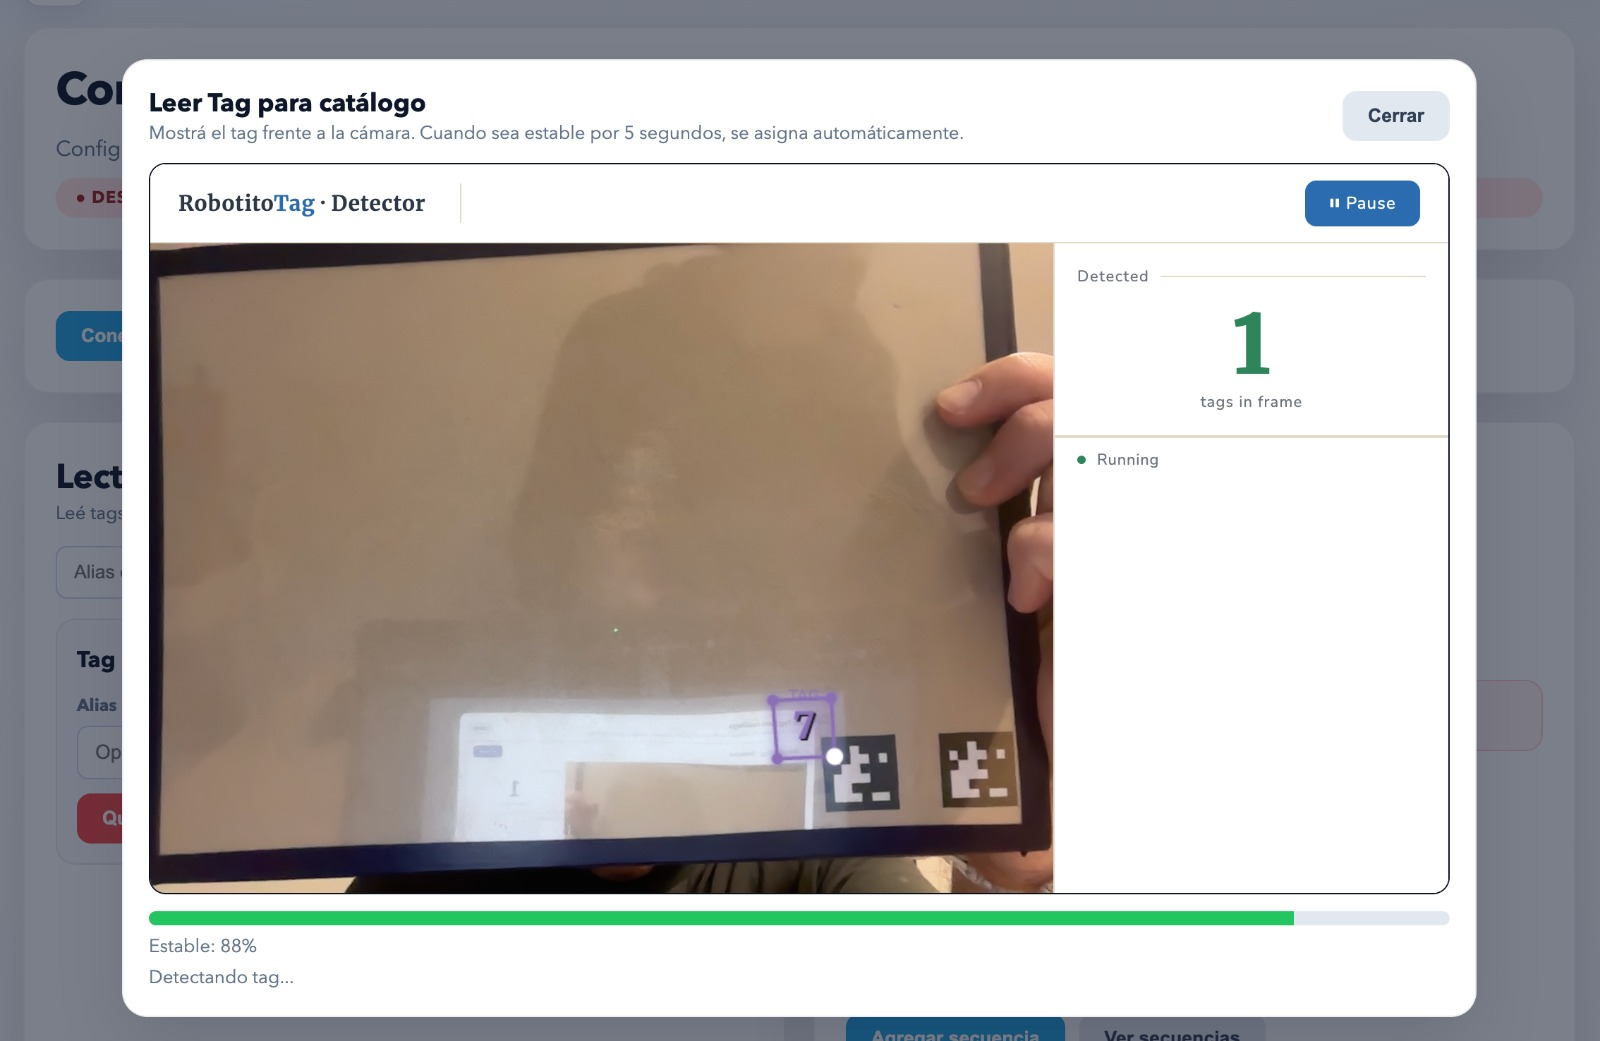
\includegraphics[width=1.3\textwidth]{images/web/tags.jpeg}
    }
    \caption{Lectura de tags.}
    \label{fig:web_tags}
\end{figure}

\section{Gestión lógica de tags e intercambiabilidad}

El configurador permite asociar cada tag físico con un identificador lógico o alias. Esto facilita que el usuario trabaje con nombres comprensibles en lugar de depender únicamente de identificadores numéricos.

Además, se incorpora un mecanismo de \textit{intercambiabilidad}. Esta funcionalidad permite declarar que dos o más tags cumplen la misma función dentro de la actividad. Por ejemplo, varios tags físicos pueden representar una misma estación.

Para modelar esta relación, el sistema utiliza un grafo no dirigido:

\[
G = (V, E)
\]

donde el conjunto de vértices \(V\) representa los tags registrados en el catálogo, y el conjunto de aristas \(E\) representa las relaciones explícitas de intercambiabilidad declaradas por el usuario.

Cada relación entre dos tags se representa mediante una conexión bidireccional. A partir de estas conexiones, el configurador identifica grupos de tags equivalentes. La implementación utiliza una búsqueda en profundidad iterativa con pila para recorrer las relaciones entre tags y determinar qué tags pertenecen a un mismo grupo.

En términos funcionales, esto permite que si el tag \(A\) es intercambiable con \(B\), y \(B\) es intercambiable con \(C\), entonces los tres puedan ser tratados como parte de una misma clase de equivalencia. Este mecanismo reduce la necesidad de duplicar manualmente secuencias y permite diseñar actividades más flexibles.

\begin{figure}[!htbp]
    \centering
    \makebox[\textwidth][c]{%
        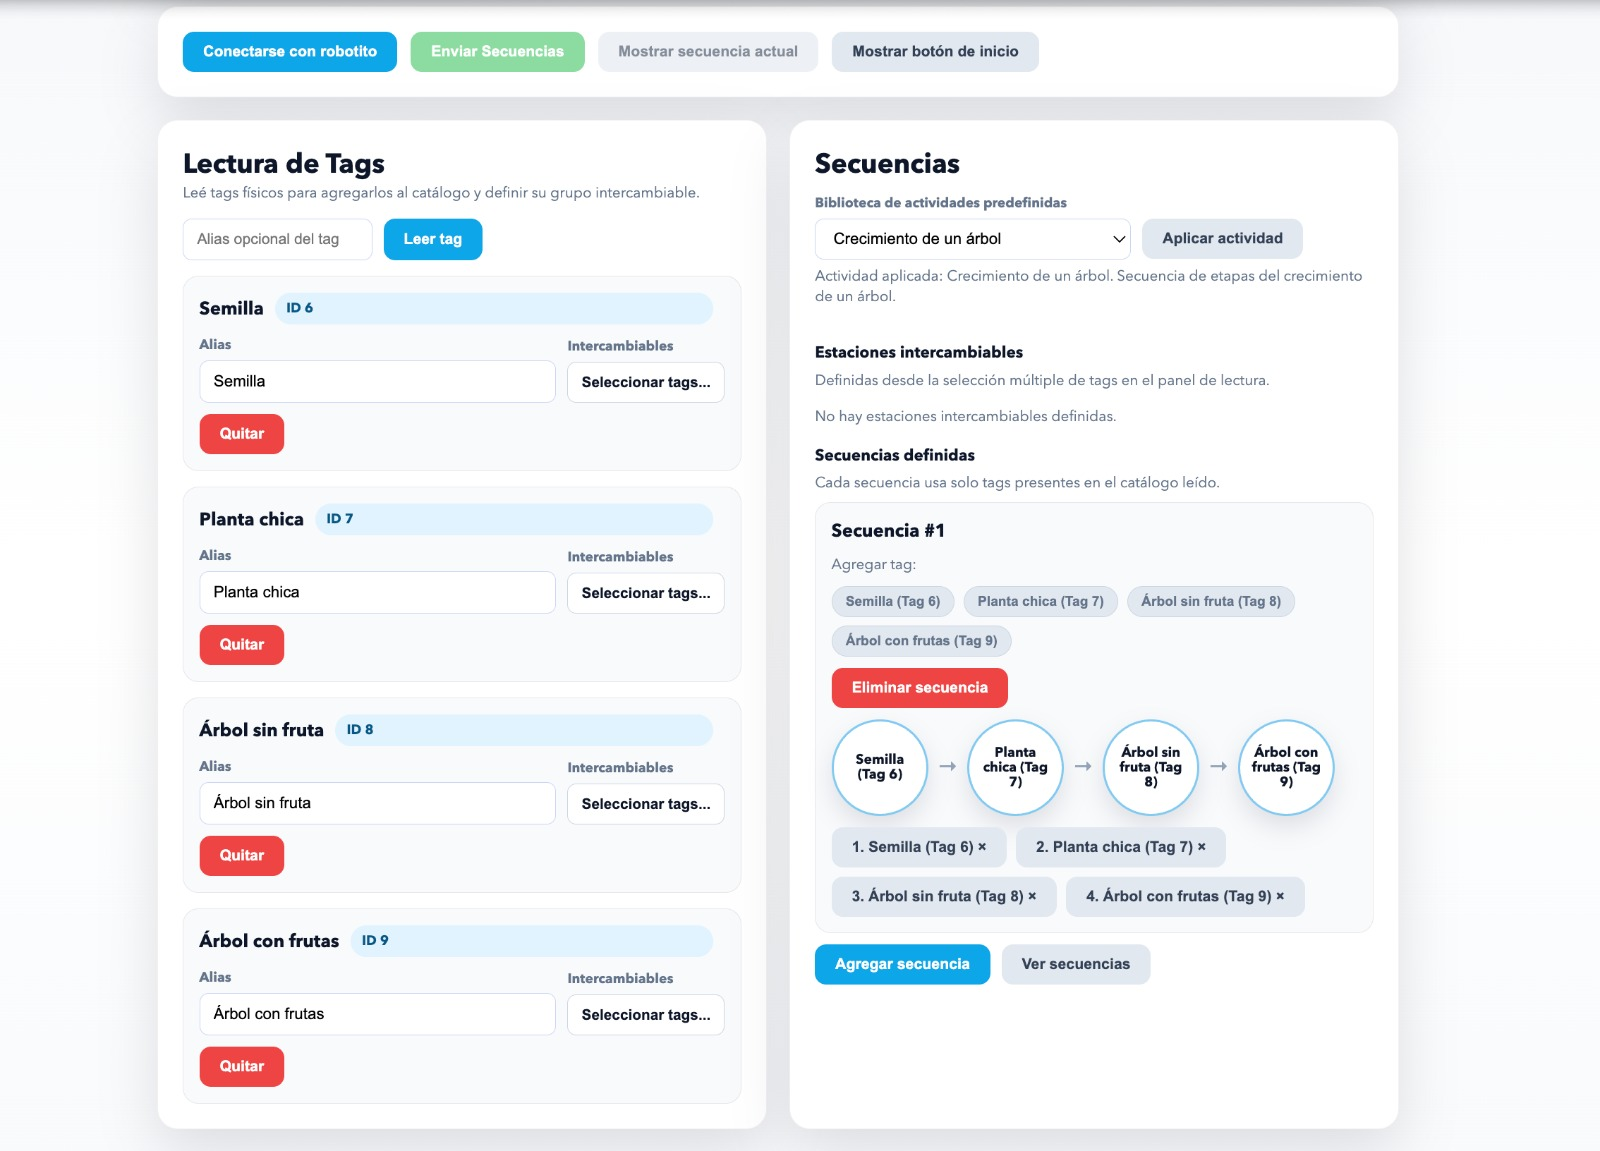
\includegraphics[width=1.3\textwidth]{images/web/secuencias.jpeg}
    }
    \caption{Gestión de secuencias.}
    \label{fig:web_secuencias}
\end{figure}

\section{Construcción y validación de secuencias}

Una vez registrados los tags o cargada una actividad predefinida, el usuario puede construir o modificar una o más secuencias de recorrido. Cada secuencia representa un orden esperado de tags que el robot deberá interpretar durante la actividad.

Antes de enviar la configuración al robot, el sistema realiza validaciones básicas para evitar inconsistencias. Entre ellas se encuentran:

\begin{itemize}
    \item verificar que exista al menos una secuencia definida;
    \item comprobar que no se supere la cantidad máxima de secuencias admitidas;
    \item validar que todos los tags usados en una secuencia estén registrados en el catálogo;
    \item impedir el uso de identificadores reservados para funciones internas del robot;
    \item detectar duplicados dentro de una misma secuencia cuando puedan generar comportamientos ambiguos.
\end{itemize}

Estas validaciones buscan prevenir errores de configuración antes de que la información sea transferida al robot.

\section{Transferencia de la configuración al robot}

Una vez validadas las secuencias, el configurador envía la información al robot mediante comunicación inalámbrica. Para esta transferencia, los datos se preparan en un formato compacto que puede ser interpretado por el firmware del robot.

La estructura enviada contiene la cantidad de secuencias, la longitud de cada una y los identificadores de los tags que la componen. Esta representación permite que el robot reciba la configuración de forma ordenada y la utilice durante la ejecución de la actividad.


\section{Biblioteca de actividades}

El configurador incorpora una biblioteca de actividades predefinidas orientada a facilitar el uso de Robotito en distintos escenarios didácticos. Esta funcionalidad permite cargar configuraciones iniciales que incluyen secuencias, grupos de tags, estaciones y relaciones de intercambiabilidad previamente definidas.

El objetivo de esta biblioteca es reducir el tiempo de preparación de cada actividad y ofrecer al usuario puntos de partida adaptados a distintos contenidos educativos. De esta manera, el docente puede seleccionar una actividad ya estructurada y luego ajustarla según las condiciones del entorno, la cantidad de tags disponibles o los objetivos específicos de la sesión.


La biblioteca de actividades no reemplaza la configuración manual, sino que la complementa. El usuario conserva la posibilidad de modificar las secuencias, editar los grupos de tags y ajustar las estaciones antes de enviar la configuración al robot.

\section{Evaluación funcional del configurador}

El configurador web aporta principalmente a la usabilidad y preparación operativa del sistema Robotito. Su principal ventaja es que permite definir recorridos y relaciones entre tags sin modificar el programa interno del robot.

Desde el punto de vista del usuario, la herramienta simplifica cuatro tareas principales:

\begin{enumerate}
    \item seleccionar una actividad predefinida o iniciar una configuración manual;
    \item registrar los tags físicos disponibles;
    \item organizar esos tags según su función en la actividad;
    \item preparar y enviar secuencias al robot.
\end{enumerate}

Como limitación, al tratarse de una herramienta auxiliar, su diseño prioriza la simplicidad y la facilidad de uso por encima de una arquitectura extensible de gran escala. En futuras versiones podría evaluarse una organización más modular si el configurador incorpora nuevas funciones, como edición avanzada de escenarios, telemetría visual o integración con otros sensores.

\section{Pruebas funcionales del sistema}

Con el objetivo de verificar que el configurador cumpla con las funcionalidades esperadas, se definió un conjunto de pruebas funcionales desde una perspectiva de aseguramiento de calidad. Estas pruebas se enfocan en el comportamiento observable del sistema y no en los detalles internos de implementación.

\renewcommand{\arraystretch}{1.25}

\begin{longtable}{L{0.10\textwidth} L{0.25\textwidth} L{0.33\textwidth} L{0.26\textwidth}}
\caption{Pruebas funcionales del configurador web}
\label{tab:pruebas-funcionales-configurador}\\
\toprule
\textbf{ID} & \textbf{Requerimiento / funcionalidad} & \textbf{Prueba realizada} & \textbf{Resultado esperado} \\
\midrule
\endfirsthead

\toprule
\textbf{ID} & \textbf{Requerimiento / funcionalidad} & \textbf{Prueba realizada} & \textbf{Resultado esperado} \\
\midrule
\endhead

PF-01 & Registro de tags físicos mediante cámara & Presentar un marcador físico válido frente a la cámara y verificar que el sistema lo detecte e incorpore al catálogo. & El tag detectado queda registrado en el catálogo de tags disponibles. \\
\midrule

PF-02 & Prevención de registros ambiguos & Presentar más de un marcador físico simultáneamente frente a la cámara. & El sistema evita registrar automáticamente una lectura ambigua. \\
\midrule

PF-03 & Confirmación de lectura estable & Presentar un marcador frente a la cámara y verificar que el sistema no lo registre ante una detección inestable o interrumpida. & El tag solo se incorpora cuando la lectura cumple la condición de estabilidad definida por el sistema. \\
\midrule

PF-04 & Asignación de alias lógico a un tag & Seleccionar un tag registrado y asignarle un nombre o alias representativo. & El sistema guarda el alias y lo muestra asociado al tag correspondiente. \\
\midrule

PF-05 & Edición del catálogo de tags & Modificar la información asociada a un tag previamente registrado. & El catálogo refleja correctamente los cambios realizados. \\
\midrule

PF-06 & Definición de intercambiabilidad entre tags & Registrar dos tags y declarar que son intercambiables. & El sistema reconoce ambos tags como equivalentes dentro de la configuración. \\
\midrule

PF-07 & Intercambiabilidad transitiva entre tags & Declarar que un tag A es intercambiable con B, y que B es intercambiable con C. & El sistema agrupa A, B y C dentro de una misma clase de equivalencia funcional. \\
\midrule

PF-08 & Construcción de una secuencia de recorrido & Crear una secuencia utilizando tags previamente registrados en el catálogo. & La secuencia queda creada con el orden de tags definido por el usuario. \\
\midrule

PF-09 & Validación de existencia de secuencias & Intentar enviar la configuración sin haber definido ninguna secuencia. & El sistema impide el envío e informa que no existen secuencias válidas para transferir. \\
\midrule

PF-10 & Validación de referencias al catálogo & Crear o intentar enviar una secuencia que contenga un tag no registrado en el catálogo. & El sistema impide el envío de la configuración inconsistente. \\
\midrule

PF-11 & Validación de identificadores reservados & Intentar utilizar en una secuencia un identificador reservado para funciones internas del robot. & El sistema rechaza el uso del identificador reservado como hito ordinario de recorrido. \\
\midrule

PF-12 & Validación de duplicados dentro de una secuencia & Crear una secuencia con un mismo tag repetido cuando dicha repetición no esté permitida. & El sistema detecta la duplicación e impide enviar una secuencia ambigua. \\
\midrule

PF-13 & Validación de cantidad máxima de secuencias & Intentar crear o enviar una cantidad de secuencias superior al límite definido por el sistema. & El sistema impide superar la cantidad máxima admitida. \\
\midrule

PF-14 & Transferencia de configuración válida al robot & Crear una configuración válida y ejecutar la acción de envío al robot. & El sistema permite la transferencia de la configuración al robot. \\
\midrule

PF-15 & Bloqueo de transferencia ante configuración inválida & Crear una configuración con errores de validación e intentar enviarla al robot. & El sistema bloquea la transferencia hasta que los errores sean corregidos. \\
\midrule

PF-16 & Carga de actividad predefinida & Seleccionar una actividad desde la biblioteca del configurador. & El sistema carga las secuencias, grupos, estaciones y tags asociados a la actividad seleccionada. \\
\midrule

PF-17 & Edición de actividad predefinida & Cargar una actividad desde la biblioteca y modificar sus secuencias o grupos de tags. & El sistema permite ajustar la actividad antes de transferir la configuración al robot. \\
\midrule

PF-18 & Usabilidad básica del flujo completo & Seleccionar o configurar una actividad, registrar tags, asignar alias, definir intercambiabilidad, crear una secuencia válida y enviarla al robot. & El usuario puede completar el flujo funcional principal del configurador sin modificar el firmware del robot. \\
\bottomrule


\end{longtable}


%%%%%%%%%%%%%%%%%%%%%%%%%%%%%%%%%%%%%%%%%%%%%%%%%%%%%%%%%%%%%%%%%%%%%%%%%%%%%%%%%%%%%%%%%%%%%%%%

% experimentación
\chapter{Experimentación}

\section{Introducción}
La validación de plataformas educativas requiere no solo verificar su funcionamiento técnico, sino también evaluar su adecuación pedagógica y usabilidad en contextos reales de enseñanza. En este capítulo se describe el proceso de experimentación llevado a cabo para validar la propuesta de extensión de Robotito, tanto desde la perspectiva docente como desde la experiencia directa con estudiantes.
La experimentación se estructuró en dos etapas complementarias: primero, entrevistas semiestructuradas con docentes de nivel inicial y primaria para obtener retroalimentación sobre el diseño de las actividades y la viabilidad práctica de la propuesta; segundo, sesiones presenciales con grupos de estudiantes de educación inicial (entre 4 y 5 años de edad) y educación primaria (entre 7 y 8 años de edad) para observar la interacción directa con el robot y validar los supuestos de diseño.

\section{Entrevistas con docentes}

Se realizaron entrevistas semiestructuradas con dos maestras de educación inicial y primaria: Elisa y Cecilia. Ambas docentes cuentan con experiencia en la integración de tecnología en el aula y habían trabajado previamente con robótica educativa en sus instituciones. Si bien no es necesario tener conocimientos tecnológicos o haber realizado algún tipo de actividad similar para poder utilizar Robotito como herramienta de enseñanza, fue beneficioso que sí lo hayan hecho ya que pudieron brindar comentarios útiles en base a experiencias previas que aportaron valor a la versión final del robot y de las actividades definidas.
Las entrevistas tuvieron una duración aproximada de 50 a 60 minutos cada una y siguieron un guión diseñado para abordar los siguientes aspectos:

\begin{enumerate}
\item \textbf{Contexto y materiales físicos}: Evaluación de la propuesta de usar piezas de tatami tipo puzzle para formar la pista del robot, la claridad de los elementos visuales (calles blancas con líneas negras, puntos de parada rojos, similitud con calles y señales de tránsito) y la viabilidad de que los niños armen el circuito de forma autónoma.
\item \textbf{Sistema de tarjetas con códigos QR}: Opinión sobre el uso de códigos QR para que el robot pueda leer y validar secuencias, la necesidad de herramientas auxiliares para que los docentes identifiquen el orden correcto de las tarjetas, y estrategias para evitar que los niños memoricen las secuencias según los códigos asociados.
\item \textbf{Retroalimentación del robot}: Tipos de feedback considerados apropiados (visual, sonoro, cinético) ante aciertos y errores, estrategias para manejar la frustración y momento adecuado para entregar la retroalimentación (paso a paso vs. al final del recorrido).
\item \textbf{Dinámica de juego y motivación}: Duración ideal de las actividades, balance entre trabajo colaborativo e individual, tipos de contenido más atractivos (cuentos, palabras, desafíos motrices), y estrategias de cierre.
\item \textbf{Aplicabilidad curricular}: Posibles integraciones con contenidos de diferentes áreas (lenguaje, matemática, ciencias naturales, etc.) y adaptabilidad a distintos niveles educativos.
\item \textbf{Consideraciones prácticas}: Dificultades previstas en términos de tiempo, espacio físico, desarrollo motriz de los niños y nivel de atención esperado.
\end{enumerate}

Las entrevistas se realizaron de forma remota mediante videollamada, con consentimiento explícito de las participantes para el uso de la información obtenida con fines de investigación educativa.

\section{Primera sesión práctica con estudiantes}
Posteriormente se organizó una sesión presencial en coordinación con la maestra Cecilia, quien facilitó el acceso a dos grupos de estudiantes de segundo año de educación primaria (niños entre aproximadamente siete y ocho años) con aproximadamente treinta alumnos en total. La actividad se realizó en el salón de clases de la institución educativa.

La sesión se estructuró en etapas progresivas, siguiendo las recomendaciones surgidas de las entrevistas:
\begin{enumerate}
\item \textbf{Discusión previa}: Conversación general sobre la tecnología y la robótica en el día a día.
\item \textbf{Presentación del robot}: Introducción de Robotito y demostración de sus capacidades básicas de movimiento.
\item \textbf{Exploración de materiales}: Manipulación de las piezas de tatami por parte de los estudiantes, observación de las líneas negras y los puntos de parada rojos, e interacción con las tarjetas con códigos QR e imágenes.
\item \textbf{Deducciones}: Etapa de conversación grupal en el que los niños presentan ideas y sugerencias sobre el funcionamiento esperado del robot.
\item \textbf{Construcción del circuito}: En grupos colaborativos, los niños armaron circuitos simples de 3 a 4 puntos de parada.
\item \textbf{Explicación del sistema de validación}: Se presentó el concepto de secuencia correcta y el rol de los códigos QR.
\item \textbf{Ejecución y retroalimentación}: Recorrido del robot por los circuitos armados por los estudiantes, validando las secuencias mediante la lectura de códigos QR y proporcionando retroalimentación inmediata con luces LED (verde para aciertos, rojo para errores).
\item \textbf{Acercamiento final}: Momento de acercamiento por parte de los niños para hacer preguntas y ver el robot de cerca, una vez finalizada la actividad y desarmado el recorrido.
\end{enumerate}

Durante la sesión se realizaron observaciones sistemáticas sobre:
\begin{itemize}
\item Nivel de comprensión de las instrucciones
\item Grado de autonomía en el armado del circuito
\item Capacidad de comprensión del sistema de validación por códigos QR
\item Nivel de atención y motivación sostenida
\item Reacciones emocionales ante aciertos y errores del robot
\item Dinámicas de colaboración entre pares
\end{itemize}

\section{Segunda sesión práctica con estudiantes}
En coordinación con la maestra Maria José se organizó otra instancia de actividad práctica, esta vez en otro jardín y con niños de educación inicial (entre cuatro y cinco años). La actividad se realizó en un salón neutro de la institución educativa, esta vez con un grupo reducido de aproximadamente diez alumnos.

La sesión se estructuró en etapas progresivas con algunas diferencias con respecto a la actividad anterior, principalmente debido a la diferencia de edad entre los grupos:
\begin{enumerate}
\item \textbf{Presentación del robot y discusión}: Introducción de Robotito y conversación sobre sus capacidades de movimiento.
\item \textbf{Exploración de materiales}: Manipulación de las piezas de tatami por parte de los estudiantes, observación de las líneas negras y los puntos de parada rojos.
\item \textbf{Construcción del circuito}: Armado de circuitos simples de 3 a 4 puntos de parada.
\item \textbf{Explicación del sistema de validación}: Se presentó el concepto de secuencia correcta y el rol de las tarjetas.
\item \textbf{Ejecución y retroalimentación}: Recorrido del robot por los circuitos armados por los estudiantes, validando las secuencias mediante la lectura de códigos QR y proporcionando retroalimentación inmediata con luces LED (verde para aciertos, rojo para errores).
\item \textbf{Acercamiento final}: Momento de acercamiento por parte de los niños para hacer preguntas y ver el robot de cerca, una vez finalizada la actividad y desarmado el recorrido.
\end{enumerate}

En esta instancia no se pone énfasis en el concepto y utilidad de los códigos QR. Según comentarios de las maestras se decide mejor realizar la actividad teniendo como foco principal el manejo del robot y el concepto de secuencia correcta y secuencia errónea.

\section{Retroalimentación de las entrevistas docentes}

Las entrevistas arrojaron comentarios sobre varios aspectos del diseño que se detallan a continuación.

\subsection{Diseño de materiales y elementos visuales}
Las docentes validaron positivamente la propuesta de usar piezas de tatami modulares como base física del juego. Consideraron que el formato de puzzle es familiar para los niños y facilita tanto el armado colaborativo como la reconfiguración del circuito para diferentes actividades. Sin embargo, sugirieron considerar la durabilidad de los materiales, especialmente de los pegotines de calle con línea negra adheridas, dado el uso intensivo esperado.
Respecto a los puntos de parada, ambas docentes recomendaron reforzar la señal visual del círculo rojo con elementos adicionales que hagan más explícita la acción esperada. Propusieron agregar íconos complementarios como ojos, manos o señales de ``PARE'' que los niños puedan asociar inmediatamente con la acción de detenerse.
\subsection{Sistema de tarjetas con códigos QR}
El diseño propuesto de tarjetas---con un código QR pequeño para la validación técnica ubicado en una esquina y una imagen central grande para los niños---fue bien recibido. Las maestras destacaron que esta dualidad permite que el contenido educativo sea visualmente predominante, mientras que el aspecto técnico queda en segundo plano.
Elisa y Cecilia plantearon la necesidad de contar con una herramienta auxiliar (aplicación móvil o sistema web) que les permita a los docentes identificar rápidamente qué código QR corresponde a cada tarjeta (o qué posición en la secuencia) al momento de preparar las actividades. Sugirieron también implementar un sistema de codificación visual en los bordes de las tarjetas (colores o patrones) que facilite la organización del material sin depender exclusivamente de la tecnología.
Para evitar que los niños memoricen las secuencias por la ubicación física de las tarjetas, propusieron implementar un sistema de rotación de códigos QR, para que en distintas sesiones identifiquen distintos pasos de la secuencia propuesta.
\subsection{Progresión pedagógica y etapas diferenciadas}
Una de las recomendaciones más consistentes fue la necesidad de presentar la actividad en etapas claramente diferenciadas, especialmente para niños más pequeños (3 a 5 años). Elisa propuso la siguiente secuencia de complejidad creciente:
\begin{enumerate}
\item \textbf{Etapa inicial}: Introducción al robot y seguimiento libre de líneas sin puntos de parada ni validación.
\item \textbf{Etapa intermedia}: Incorporación de puntos de parada rojos sin validación de secuencia (el robot simplemente se detiene).
\item \textbf{Etapa avanzada}: Introducción del sistema completo con validación de códigos QR y retroalimentación.
\end{enumerate}
Esta progresión permite que los niños comprendan gradualmente cada componente del sistema antes de enfrentarse a la actividad completa.
\subsection{Retroalimentación del robot}
Las docentes coincidieron en que la retroalimentación inmediata es fundamental para el aprendizaje, pero debe diseñarse cuidadosamente para no generar frustración excesiva. Recomendaron un sistema de retroalimentación visual mediante luces LED de colores:
\begin{itemize}
\item \textbf{Verde}: Imagen en la posición correcta dentro de la secuencia.
\item \textbf{Rojo}: Imagen en una posición incorrecta dentro de la secuencia.
\end{itemize}
Para el manejo de errores, sugirieron evitar que el robot vuelva automáticamente al inicio tras cada error, ya que esto podría resultar frustrante. En su lugar, propusieron que el robot se detenga en el punto de error, emita la señal visual correspondiente y espere a que los niños corrijan la tarjeta antes de continuar. Esta estrategia mantiene el flujo de la actividad y convierte el error en una oportunidad de reflexión y corrección inmediata.
Al completar exitosamente toda la secuencia, las maestras sugirieron una celebración multimodal: combinación de luces verdes parpadeantes, sonido festivo y, si es posible, algún movimiento expresivo del robot (giro, baile simple).
\subsection{Control del flujo de la actividad}
Un aspecto crítico identificado durante las entrevistas fue la necesidad de que los docentes puedan controlar el flujo de ejecución de la actividad. Las maestras plantearon dos situaciones recurrentes en el aula que requerían funcionalidades específicas:
\paragraph{Función de pausa} Los docentes necesitan poder detener el robot en cualquier momento del recorrido para realizar intervenciones pedagógicas oportunas. Situaciones típicas incluyen:
\begin{itemize}
\item Aprovechar un momento de error para generar una discusión grupal sobre la secuencia correcta
\item Atender interrupciones externas (llegada de otro docente, situaciones de convivencia)
\item Permitir que todos los niños del grupo puedan observar un momento específico del recorrido
\item Dar tiempo a los niños para reflexionar sobre lo que el robot hará a continuación
\end{itemize}
\paragraph{Función de reinicio (reset)} La posibilidad de volver a comenzar el recorrido desde cero sin necesidad de apagar y encender el robot resultó fundamental para la dinámica del aula. Esta funcionalidad es necesaria para:
\begin{itemize}
\item Permitir múltiples intentos de la misma secuencia sin interrupciones técnicas
\item Facilitar que diferentes grupos de niños prueben sus propias configuraciones
\item Corregir errores de configuración inicial sin perder tiempo en reinicios manuales
\item Mantener el ritmo de la clase cuando se trabaja con actividades breves y repetitivas
\end{itemize}
Estas sugerencias evidenciaron que el robot no solo debe ejecutar secuencias de manera autónoma, sino también ofrecer puntos de control que permitan al docente mantener la gestión pedagógica de la actividad.
\subsection{Aplicaciones curriculares}
Las docentes identificaron múltiples posibilidades de integración curricular. La plataforma permite trabajar con secuencias asociadas a diversas áreas: narrativas de cuentos tradicionales en lenguaje y literatura, procesos naturales como el ciclo de vida de una planta en ciencias naturales, secuencias numéricas y patrones en matemática, o recorridos espaciales que conecten diferentes contextos sociales. Particularmente valoraron la posibilidad de que los niños creen sus propias secuencias mediante dibujos, otorgando mayor sentido de autoría a la actividad.

\subsection{Duración y organización de las actividades}
Las maestras recomendaron limitar las secuencias a 3-5 puntos de parada para niños de nivel inicial y primeros años de primaria. Actividades más largas podrían provocar pérdida de atención y dificultad para mantener en mente la secuencia completa.
En cuanto a la duración total de la sesión, sugirieron bloques de 20 a 30 minutos, incluyendo tiempo para el armado colaborativo del circuito, la ejecución y la reflexión posterior. Consideraron fundamental incluir un momento final de cierre donde los niños puedan verbalizar lo que hicieron y aprendieron.
Respecto a la organización, propusieron dinámicas de trabajo en pequeños grupos (3-4 niños) donde se puedan asignar roles rotativos: diseñador del circuito, colocador de tarjetas, observador del robot, y registrador de resultados. Esta distribución de roles fomenta la participación equitativa y el desarrollo de diferentes habilidades.
\section{Observaciones de la primera sesión con estudiantes}
La sesión presencial con los dos grupos de segundo año de primaria permitió validar varios de los supuestos de diseño y observar directamente la interacción de los niños con el sistema.
\subsection{Comprensión del sistema}
Los estudiantes comprendieron rápidamente el concepto de seguimiento de línea y la función de los puntos de parada rojos. La analogía con las señales de tránsito (semáforo rojo = detenerse) facilitó la comprensión inmediata del sistema.

Un aspecto interesante observado durante la actividad fue la tendencia de los niños a asimilar el robot, o algunas de sus partes, con características humanas. Por ejemplo, varios estudiantes interpretaron la cámara como los ``ojos'' del robot y las ruedas como sus ``piernas''. Estas asociaciones espontáneas facilitaron la construcción de una representación intuitiva del sistema, ya que permitieron vincular componentes técnicos con referencias corporales conocidas por los niños.

Esta forma de interpretación también permitió introducir, de manera implícita, la idea de modularización del robot. Al reconocer que distintas partes cumplen funciones específicas, como ver, moverse o detectar elementos del entorno, se vuelve más comprensible que el robot pueda extender sus capacidades mediante la incorporación de nuevos módulos. En este sentido, la cámara no se percibe únicamente como un accesorio agregado, sino como una funcionalidad adicional que amplía lo que Robotito puede hacer.

Por otro lado, el concepto de secuencia correcta fue inicialmente más abstracto. Algunos niños asumieron que cualquier orden de las tarjetas sería válido. Sin embargo, al presentar ejemplos concretos con narrativas conocidas, la lógica de la secuencia se volvió evidente.

La función de los códigos QR como mecanismo de validación técnica no fue completamente comprendida por todos los niños, pero tampoco resultó necesario que lo comprendieran en profundidad. Para ellos, el robot ``sabía'' si la tarjeta era correcta, lo cual era suficiente para participar en la actividad.
\subsection{Autonomía en el armado}
Los estudiantes de segundo año demostraron capacidad para armar circuitos simples de forma relativamente autónoma. Trabajando en grupos de 3-4 niños, lograron conectar las piezas de tatami siguiendo instrucciones básicas. Hubo algunos casos de piezas colocadas en orientaciones incorrectas (línea discontinua, ángulos cerrados), pero con mínima intervención del adulto lograron identificar y corregir los errores.
La colocación de las tarjetas sobre los puntos de parada requirió mayor guía inicial. Algunos niños intentaron colocar múltiples tarjetas en un mismo punto o no alineaban correctamente la tarjeta para que el robot pudiera leer el código QR. Tras una demostración y práctica, mejoraron significativamente en esta tarea.
\subsection{Motivación y compromiso}
El nivel de motivación fue consistentemente alto durante toda la sesión. Los niños mostraron gran entusiasmo al ver al robot en movimiento y mantuvieron la atención durante las explicaciones cuando estas estaban acompañadas de demostraciones prácticas.

Los niños celebraban espontáneamente cuando el robot completaba exitosamente una secuencia, lo que sugiere que la actividad genera un sentido genuino de logro.
\subsection{Reacción ante errores}
Las señales de error (luz roja) no generaron frustración significativa. En la mayoría de los casos, los niños reaccionaron con curiosidad, intentando identificar qué tarjeta estaba en el lugar incorrecto. La recomendación docente de no hacer que el robot vuelva al inicio resultó acertada: permitir que los niños corrigieran el error in situ mantuvo el flujo de la actividad y convirtió el error en una oportunidad de aprendizaje inmediato.
\subsection{Colaboración}
Las dinámicas colaborativas funcionaron bien en general. Los niños negociaban espontáneamente quién colocaba cada tarjeta y se ayudaban mutuamente a identificar errores. Sin embargo, en algunos grupos surgieron conflictos menores por el control del material o diferencias de opinión sobre el orden correcto.
La maestra Cecilia intervino en estos casos sugiriendo turnos rotativos y promoviendo el diálogo sobre las razones de cada propuesta, lo que resultó en una experiencia más enriquecedora.

\section{Observaciones de la segunda sesión con estudiantes}
La segunda sesión presencial, realizada con un grupo de educación inicial de entre cuatro y cinco años, permitió observar la interacción de niños más pequeños con la plataforma. A diferencia de la primera instancia, el grupo fue reducido, con aproximadamente diez estudiantes, lo que permitió una dinámica más controlada y un acompañamiento más cercano por parte de las maestras.
\subsection{Comprensión del sistema}
Debido a la edad de los niños, la comprensión inicial del concepto de robot fue menos precisa que en la primera sesión. Algunos estudiantes asociaron Robotito con una aspiradora robot, utilizando como referencia un objeto tecnológico más familiar en su entorno cotidiano. Si bien estas asociaciones no describían correctamente el propósito del sistema, sí funcionaron como punto de partida para comprender que se trataba de un dispositivo capaz de desplazarse de forma autónoma.

Los niños lograron identificar progresivamente que el robot podía moverse sobre el circuito y detenerse ante ciertas señales. Las señales de parada rojas resultaron especialmente comprensibles, ya que varios estudiantes las relacionaron con la idea de detenerse o esperar. Asimismo, manifestaron curiosidad por la cámara incorporada al robot, realizando preguntas o comentarios sobre su posible función.
\subsection{Rol de las docentes durante la actividad}
En esta instancia, la actividad requirió una mediación docente más fuerte que en la sesión anterior. Las maestras guiaron de forma más directa la presentación del robot, el armado del circuito y la interpretación de lo que ocurría durante el recorrido. Esta intervención fue necesaria debido a la edad de los estudiantes y permitió mantener la atención del grupo, ordenar la participación y traducir las consignas a explicaciones más concretas.

A diferencia de la primera sesión, no se generaron instancias extensas de discusión o debate colectivo. Sin embargo, los niños sí participaron mediante comentarios breves, preguntas espontáneas e intentos de anticipar qué debía hacer el robot en cada paso. Esto evidenció que, aunque la actividad debió ser más guiada, seguía habilitando formas iniciales de razonamiento sobre movimiento, secuencia y respuesta del sistema.
\subsection{Participación e interés}
La respuesta general de los estudiantes fue muy positiva. Una gran mayoría del grupo se mostró interesada en el robot, observó con atención sus movimientos y participó activamente cuando se les preguntaba qué debía ocurrir a continuación. Varios niños realizaron aportes espontáneos sobre el recorrido, las señales de parada y la función de los elementos visibles del robot.

El tamaño reducido del grupo favoreció que los estudiantes pudieran acercarse, observar el robot con mayor detalle y expresar ideas durante la actividad. Si bien las intervenciones no siempre fueron técnicamente acertadas, sí demostraron curiosidad y disposición a interactuar con la propuesta.
\subsection{Adecuación de la actividad para educación inicial}
La sesión permitió comprobar que la propuesta también resulta atractiva para niños de educación inicial, aunque requiere ajustes en la forma de presentación y en el grado de acompañamiento docente. Para este rango etario, la actividad debe apoyarse principalmente en consignas concretas, observación directa del comportamiento del robot y participación guiada en cada etapa del recorrido.

En este sentido, la actividad funcionó adecuadamente cuando fue presentada de forma breve, visual y altamente mediada por las maestras. La experiencia mostró que los niños de cuatro y cinco años pueden comprender qué hace el robot, identificar situaciones simples como el movimiento y la detención ante señales, y participar en la toma de decisiones durante la actividad, aunque todavía no logren formular con precisión qué es un robot o explicar su funcionamiento de manera abstracta.

\section{Análisis y discusión}
Los resultados de la experimentación validan la viabilidad tanto técnica como pedagógica de la propuesta. La integración de la cámara HuskyLens con el sistema de códigos QR funciona de manera confiable en condiciones reales de aula, y el diseño de la actividad resulta comprensible y motivador para los estudiantes del rango etario objetivo.
\subsection{Fortalezas identificadas}
\paragraph{Tangibilidad y manipulación física} El uso de materiales físicos (piezas de tatami, tarjetas) favorece el aprendizaje activo y permite que niños con diferentes estilos de aprendizaje se involucren en la actividad. La posibilidad de reconfigurar el circuito otorga un sentido de agencia y creatividad.
\paragraph{Retroalimentación inmediata y visible} El sistema de luces LED proporciona retroalimentación clara, inmediata y no verbal, lo cual es especialmente apropiado para niños pequeños. La retroalimentación visual evita la necesidad de mediación constante del adulto.
\paragraph{Adaptabilidad curricular} La plataforma no está atada a un contenido específico, lo que permite a los docentes integrarla de forma flexible en diferentes áreas y niveles educativos. Esta versatilidad aumenta significativamente su potencial de uso sostenido.
\paragraph{Aprendizaje colaborativo} El diseño natural de la actividad promueve el trabajo en equipo, la negociación y el diálogo, habilidades fundamentales en el desarrollo infantil.
\paragraph{Progresión de complejidad} La posibilidad de utilizar el sistema en diferentes niveles de complejidad (desde seguimiento simple de línea hasta validación completa de secuencias) permite adaptarlo a distintos grupos etarios y niveles de desarrollo.
\subsection{Desafíos y áreas de mejora}
\paragraph{Curva de aprendizaje inicial} Los estudiantes de segundo año de primaria con quienes se realizó la sesión práctica lograron comprender e integrar todos los elementos del sistema (armado del circuito, comprensión de secuencias y validación por códigos QR) dentro de una misma sesión de clase. Sin embargo, para niños de edades más tempranas, es probable que sea necesario planificar sesiones introductorias progresivas que presenten cada componente por separado, tal como sugirieron las docentes entrevistadas.
\paragraph{Gestión de materiales} El sistema requiere múltiples componentes (piezas de tatami, tarjetas, robot) que deben organizarse, almacenarse y mantenerse. Esto puede representar una carga logística para los docentes, especialmente si trabajan con grupos numerosos o tienen limitaciones de espacio físico.
\paragraph{Necesidad de control del flujo de actividad} La experiencia inicial mostró que sin mecanismos de pausa y reinicio, los docentes iban a tener dificultades para gestionar el ritmo de la clase. La imposibilidad de detener el robot para hacer intervenciones pedagógicas o de reiniciar rápidamente para nuevos intentos se determinó como limitante para la flexibilidad de uso en el aula. Este feedback fue determinante para la incorporación de los controles de flujo mencionados.
\paragraph{Dependencia de elementos técnicos} Aunque el sistema es robusto, depende del correcto funcionamiento de la cámara y de la lectura de códigos QR. En la primera sesión con estudiantes se observó una falla de lectura asociada a las condiciones de iluminación del salón, dado que en ese momento el robot utilizaba reconocimiento de colores para identificar las zonas de parada. Esta situación motivó un ajuste en el funcionamiento del sistema: las acciones del recorrido dejaron de depender de la detección de colores y pasaron a ser activadas mediante la lectura de códigos QR. A partir de este cambio, la lógica principal de la actividad quedó basada en el seguimiento de líneas y el reconocimiento de códigos QR, reduciendo la dependencia respecto a la iluminación ambiente para la detección de los puntos de parada. De todos modos, códigos QR dañados, mal alineados o mal ubicados pueden interrumpir la actividad, por lo que es importante desarrollar protocolos para el mantenimiento y la resolución rápida de este tipo de problemas.
\paragraph{Necesidad de herramientas auxiliares para docentes} La solicitud de una herramienta que permita a los docentes identificar códigos QR mediante sus teléfonos móviles es legítima y necesaria. Sin esta herramienta, la preparación de actividades se vuelve más compleja y propensa a errores.
\paragraph{Riesgo de memorización} Sin un sistema de rotación de códigos QR, los niños podrían memorizar posiciones físicas en lugar de razonar sobre secuencias lógicas. Esto disminuiría el valor educativo de la actividad.
\subsection{Validación de decisiones de diseño}
La experimentación validó varias decisiones de diseño tomadas durante el desarrollo:
\begin{enumerate}
\item \textbf{Uso de HuskyLens sobre otras cámaras}: La capacidad de reconocimiento confiable de códigos QR en tiempo real demostró ser adecuada para el contexto educativo. La alternativa de procesamiento remoto habría agregado complejidad innecesaria.
\item \textbf{Eliminación del reconocimiento de colores en puntos de parada}: La primera instancia con estudiantes permitió identificar que la detección de colores podía verse afectada por las condiciones de iluminación del salón. A partir de esta observación, se decidió que las acciones del recorrido no fueran activadas por reconocimiento de colores, sino mediante la lectura de códigos QR. Esta modificación fue validada en la segunda instancia, donde no se observaron problemas de lectura asociados a la iluminación de la sala.
\item \textbf{Retroalimentación paso a paso vs. final}: La retroalimentación inmediata en cada punto de parada resultó más efectiva pedagógicamente que esperar al final del recorrido \cite{marwan2022adaptiveFeedback}.  Permite correcciones oportunas y mantiene el foco de los niños.
\item \textbf{Sistema modular de piezas de tatami}: El formato de puzzle resultó intuitivo y práctico. La modularidad permite escalabilidad (circuitos más largos o complejos) sin requerir nuevos materiales fundamentalmente diferentes.
\item \textbf{Integración de árboles de comportamiento}: Aunque no fue visible para los usuarios finales, la arquitectura basada en Behavior Trees facilitó la implementación de la lógica de control y permitirá futuras extensiones del comportamiento del robot de forma ordenada y mantenible.
\end{enumerate}
\section{Ajustes realizados basados en el feedback}
Como resultado de la experimentación, se implementaron y planificaron diversos ajustes:
\subsection{Ajustes implementados}
\paragraph{Mejoras en señales visuales de parada} Se reforzaron los círculos rojos con iconografía adicional (señal de ``PARE'' estilizada) para hacerlos más explícitos, especialmente para niños más pequeños.
\paragraph{Calibración de retroalimentación luminosa} Se ajustó la intensidad y duración de las señales LED para que sean claramente visibles incluso en ambientes bien iluminados, pero sin resultar abrumadoras. Se define además que previo a realizar la retroalimentación luminosa el robot debe mostrarse en un estado ``pensativo'' (sin movimiento, con las luces LED ``girando'' por un segundo) para darle tiempo a los niños que entiendan exactamente qué está pasando en cada paso del recorrido.
\paragraph{Implementación de controles de flujo} En respuesta directa al feedback docente, se incorporaron dos funcionalidades esenciales:
\begin{enumerate}
\item \textbf{Función de pausa}: Se implementó un mecanismo que permite al docente detener la ejecución en cualquier momento realizando la acción de levantar el robot. Cuando se activa la pausa:
\begin{itemize}
\item El robot detiene su movimiento inmediatamente y se activa el modo ``pausa''
\item Se mantiene el contexto de la actividad (no pierde el progreso)
\item Puede reanudarse desde el mismo punto al reubicarlo en el recorrido y mostrar el QR correspondiente a ``iniciar''
\item Permite intervenciones pedagógicas sin interrumpir el flujo lógico de la secuencia
\end{itemize}
\item \textbf{Función de reset}: Se agregó una etiqueta específica (QR)  que permite reiniciar el recorrido y comenzarlo desde cero. Esta función:
\begin{itemize}
\item Reinicia el estado interno del robot (contador de secuencia, validaciones previas)
\item Posiciona virtualmente al robot al inicio del circuito
\item Limpia los registros de aciertos/errores anteriores
\item Permite comenzar una nueva ejecución rápidamente sin manipulación física del robot
\end{itemize}
\end{enumerate}
Ambas funcionalidades se diseñaron para ser accesibles en base a acciones simples, permitiendo que los docentes mantengan el control pedagógico de la actividad en tiempo real sin depender de conocimientos técnicos avanzados.
\paragraph{Documentación de progresión pedagógica} Se elaboró material de guía para docentes que describe explícitamente las tres etapas de complejidad creciente (seguimiento libre, paradas simples, validación completa) con ejemplos de actividades para cada nivel, incluyendo ahora recomendaciones sobre cuándo y cómo utilizar las funciones de pausa y reset.
\section{Conclusiones del proceso de experimentación}
La experimentación realizada demuestra que la extensión de Robotito con capacidades de visión artificial y validación de secuencias es técnicamente funcional y pedagógicamente valiosa. La plataforma logra integrar pensamiento computacional, razonamiento secuencial y contenidos curriculares diversos en una experiencia de aprendizaje tangible y motivadora.
El proceso iterativo de diseño---desde las entrevistas con docentes expertas hasta la validación práctica con estudiantes---resultó fundamental para identificar y resolver aspectos que no habrían sido evidentes desde una perspectiva puramente técnica. Las recomendaciones de las maestras sobre progresión pedagógica, gestión de la frustración y adaptabilidad curricular enriquecieron significativamente el diseño final.
Las sesiones con estudiantes confirmaron que la propuesta es accesible y atractiva para el público objetivo, aunque también evidenció la necesidad de herramientas de apoyo para los docentes y protocolos claros para el uso efectivo del sistema. En particular, la incorporación de las funciones de pausa y reset surgió como un elemento crítico para permitir que los docentes mantengan el control pedagógico de la actividad sin sacrificar la autonomía del robot.
En conjunto, la experimentación valida que Robotito extendido con visión artificial constituye una herramienta educativa viable que puede contribuir al desarrollo del pensamiento computacional y al aprendizaje de contenidos curriculares en edades tempranas, cumpliendo así con los objetivos educativos planteados en este proyecto.

%%%%%%%%%%%%%%%%%%%%%%%%%%%%%%%%%%%%%%%%%%%%%%%%%%%%%%%%%%%%%%%%%%%%%%%%%%%%%%%%%%%%%%%%%%%%%%%%

%conclusiones
\chapter{Conclusiones y Trabajo Futuro}

\section{Conclusiones}

Este trabajo extendió la plataforma educativa Robotito en cuatro dimensiones concretas: un módulo de visión artificial basado en la cámara HuskyLens, un motor de Árboles de Comportamiento implementado en Lua RTOS, un módulo de comunicación Bluetooth con persistencia en NVS, y una carcasa rediseñada para integrar la cámara de forma robusta y reproducible.

Desde el punto de vista técnico, se desarrollaron tres componentes reutilizables que extienden la plataforma de forma independiente. El módulo HuskyLens abstrae toda la complejidad del protocolo de comunicación con la cámara, exponiendo una API uniforme accesible desde C y desde Lua que permite incorporar percepción visual en futuros proyectos sin lidiar con los detalles del bus I2C ni del protocolo propietario del sensor. El motor de Árboles de Comportamiento provee una biblioteca de control general desacoplada de cualquier lógica de dominio específica, lo que permite modelar nuevos comportamientos robóticos combinando los nodos existentes sin modificar el núcleo del sistema. El módulo Bluetooth transforma a Robotito de un autómata con rutas fijas en una plataforma configurable dinámicamente desde una aplicación web, con persistencia entre sesiones mediante NVS y protección ante accesos concurrentes desde FreeRTOS y Lua. La integración de los tres módulos en el juego implementado valida que la arquitectura funciona de forma coordinada en condiciones reales de uso.

Desde el punto de vista pedagógico, la experimentación con tres maestras de nivel inicial y primaria y dos sesiones con estudiantes de entre 4 y 8 años demostró que la plataforma es accesible y motivadora para el público objetivo. Los niños de segundo año de primaria comprendieron rápidamente el mecanismo de seguimiento de línea y la lógica de secuencia correcta, apoyándose en analogías con señales de tránsito y en narrativas conocidas. Los niños de nivel inicial requirieron una mediación mayor, pero respondieron positivamente a la retroalimentación luminosa del anillo LED. En ambas sesiones el feedback inmediato en cada punto de parada ---verde para aciertos, rojo para errores--- resultó más efectivo pedagógicamente que esperar al final del recorrido. Las funciones de pausa y reset, incorporadas a partir del feedback docente, resultaron indispensables para que las maestras pudieran realizar intervenciones pedagógicas sin perder el estado del juego ni reiniciar el robot manualmente.

En conjunto, el proyecto consolida a Robotito como una plataforma abierta que integra visión artificial, control modular y conectividad inalámbrica, alineada con las tendencias internacionales en educación STEM y con capacidad real de adopción en el sistema educativo uruguayo.

\section{Líneas de trabajo futuro}

\textbf{Persistencia de modelos aprendidos en tarjeta SD.} Los modelos entrenados en la HuskyLens ---línea guía, etiqueta de inicio, etiqueta de fin y etiquetas de parada--- se almacenan en la memoria interna del dispositivo y pueden perderse si un usuario manipula accidentalmente el menú de la cámara. Guardarlos en una tarjeta SD permitiría restaurarlos automáticamente al encender el robot, eliminando la necesidad de reentrenar el sensor ante cada desconfiguración.

\textbf{Cambio dinámico de asociación QR--secuencia.} El módulo Bluetooth ya permite configurar el mapeo entre identificadores QR y posiciones de la secuencia desde la aplicación web. Una extensión natural sería permitir reasignar ese mapeo entre sesiones para que el mismo conjunto físico de tarjetas pueda representar distintas secuencias, mitigando el riesgo de que los niños memoricen posiciones físicas en lugar de razonar sobre el orden lógico.

\textbf{Retroalimentación sonora.} Complementar el feedback visual de los LEDs con señales sonoras diferenciadas para aciertos y errores enriquecería la experiencia, especialmente en grupos numerosos o con niños de menor edad, donde captar y mantener la atención del grupo completo es más desafiante.

\textbf{Bifurcaciones en el mapa.} Incorporar intersecciones en el circuito de tatami donde el robot deba elegir un camino según el resultado de la validación introduciría nociones de condicionales y ramificación lógica de forma concreta y visible, ampliando las posibilidades pedagógicas de la plataforma hacia conceptos más avanzados de programación.

\textbf{Evaluación a mayor escala.} Las dos sesiones realizadas constituyeron una validación inicial con grupos acotados en instituciones específicas. Una evaluación con múltiples docentes, niveles educativos e instituciones distintas permitiría obtener evidencia más robusta sobre el impacto pedagógico real y detectar aspectos de diseño que no emergen en contextos controlados.
 
\textbf{Aplicación auxiliar para identificación de códigos QR.} Durante la experimentación, las docentes señalaron la necesidad de contar con una herramienta que les permita identificar el orden correcto de las tarjetas QR desde sus teléfonos móviles, sin depender del robot. Desarrollar una aplicación web o móvil con esta funcionalidad reduciría la complejidad de preparación de las actividades y minimizaría errores en la configuración de las secuencias.


%%%%%%%%%%%%%%%%%%%%%%%%%%%%%%%%%%%%%%%%%%%%%%%%%%%%%%%%%%%%%%%%%%%%%%%%%%%%%%%%%%%%%%%%%%%%%%%%
% Parte final
%%%%%%%%%%%%%%%%%%%%%%%%%%%%%%%%%%%%%%%%%%%%%%%%%%%%%%%%%%%%%%%%%%%%%%%%%%%%%%%%%%%%%%%%%%%%%%%%


{ % inicio backmatter

\backmatter % no numerar capítulos 

% referencias bibliográficas

\newpage
\bibliographystyle{apacite}
\bibliography{referencias}

} % fin backmatter

%%%%%%%%%%%%%%%%%%%%%%%%%%%%%%%%%%%%%%%%%%%%%%%%%%%%%%%%%%%%%%%%%%%%%%%%%%%%%%%%%%%%%%%%%%%%%%%%

% anexos

\begin{appendix}

\chapter{Modelado de carcasa para Robotito}

Con el objetivo de obtener una versión final del robot más robusta, estética y reproducible a mayor escala, se propone el diseño de una carcasa específica para la integración de Robotito con la cámara HuskyLens. En los prototipos iniciales los módulos se fijaban mediante soportes pegados o atornillados, con cables expuestos y componentes de sujeción visibles, lo que no garantizaba estabilidad mecánica ni una configuración consistente para el correcto funcionamiento del robot. El nuevo modelo permite encapsular los componentes en una estructura única compuesta por la carcasa original de Robotito modificada y una tapa adicional, de modo que el ensamblado sea directo y siempre resulte en la misma disposición validada durante las pruebas.

El diseño se realizó en función de los requerimientos de la cámara HuskyLens, fijando su posición de forma rígida y definiendo un ángulo específico de inclinación respecto al piso, ya que estos parámetros resultaron críticos para el correcto funcionamiento de los algoritmos de visión. Además, se incorporaron orificios internos para el guiado del cableado, logrando que este quede completamente contenido dentro de la estructura. De esta manera se logra la protección de los componentes, la confiabilidad del sistema y la calidad visual del robot, resultando en un dispositivo final adaptado específicamente a la aplicación educativa.

\section{Desarrollo del diseño de la carcasa}

Para evitar modificaciones internas a la disposición de los componentes ya existentes en Robotito, todo el trabajo de rediseño se realizó en la parte externa de la carcasa original. Para esto se trabajó sobre un modelo trisimensional de la carcasa exterior original de Robotito \cite{CarcasaRobotito}, que consiste de una única pieza con dimensiones aproximadas de 16.56cm x 16.42cm x 6.15cm (largo x ancho x alto).

\begin{figure}[htbp]
    \centering

    % -------- Primera fila --------
    \begin{subfigure}{0.4\textwidth}
        \centering
        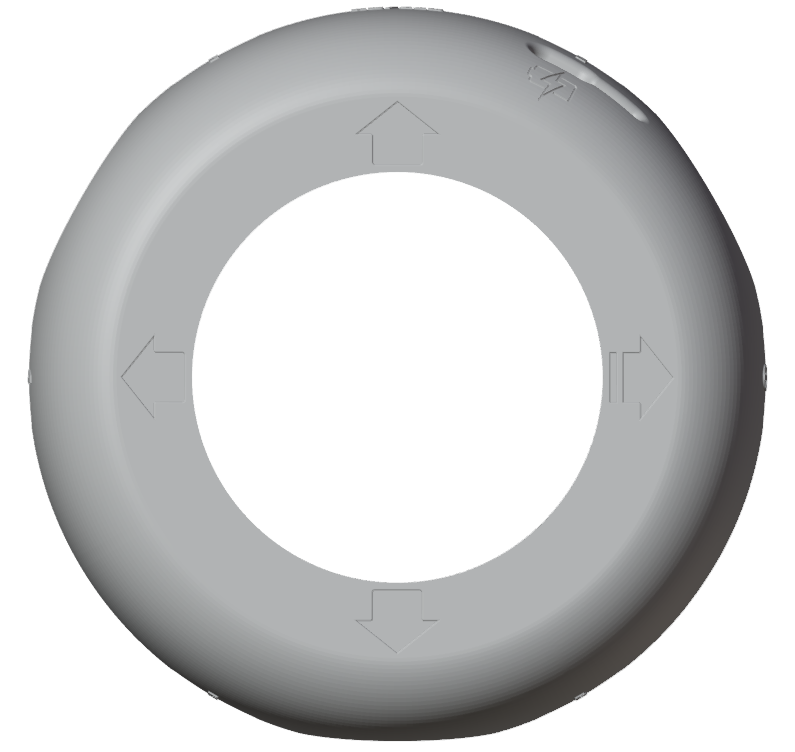
\includegraphics[width=\linewidth]{images/modelos3d/carcasa-original-superior.png}
        \caption{Vista superior}
    \end{subfigure}
    \hfill
    \begin{subfigure}{0.4\textwidth}
        \centering
        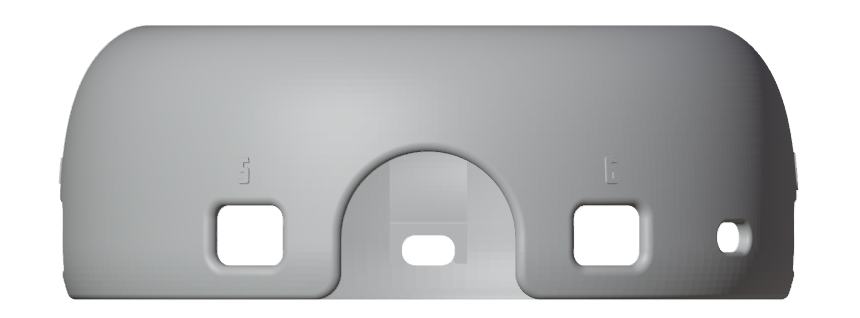
\includegraphics[width=\linewidth]{images/modelos3d/carcasa-original-frontal.png}
        \caption{Vista frontal}
    \end{subfigure}

    % -------- Segunda fila --------
    \begin{subfigure}{0.6\textwidth}
        \centering
        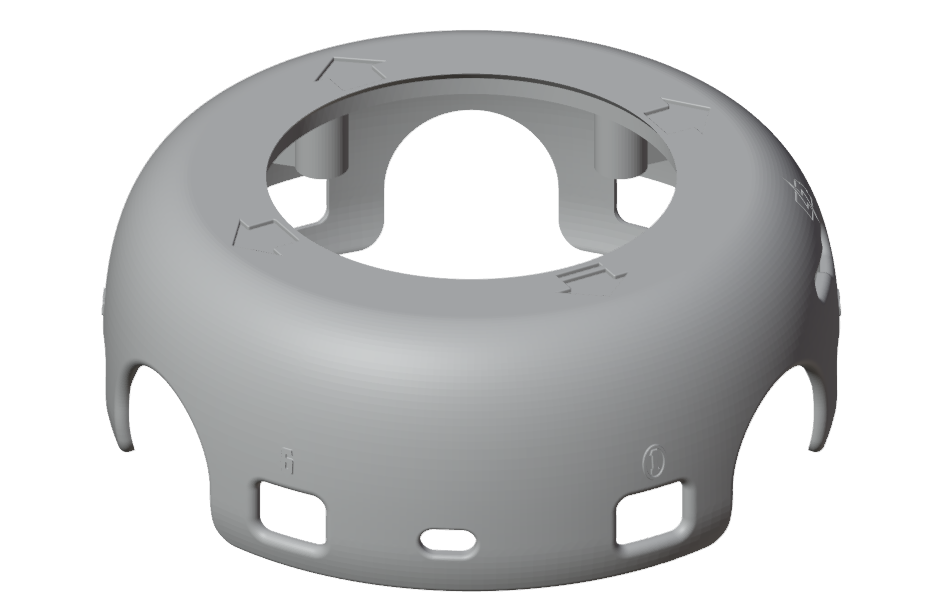
\includegraphics[width=\linewidth]{images/modelos3d/carcasa-original-3d.png}
        \caption{Vista en perspectiva}
    \end{subfigure}

    \caption{Vistas del modelo tridimensional de la carcasa original de Robotito utilizado como base para el rediseño.}
    \label{fig:carcasa-original}
\end{figure}

Además se buscaron modelos de soporte para HuskyLens, llegando a la decisión de utilizar un modelo de dos piezas (incluyendo una base y una tapa) de carcasa externa de la cámara  \cite{CarcasaHuskylens}, con dimensiones aproximadas de 5.72cm x 4.82cm x 7.3cm para la base y 5.72cm x 4.12cm x 9.6cm para la tapa.

\begin{figure}[htbp]
    \centering

    % -------- Primera fila --------
    \begin{subfigure}{0.4\textwidth}
        \centering
        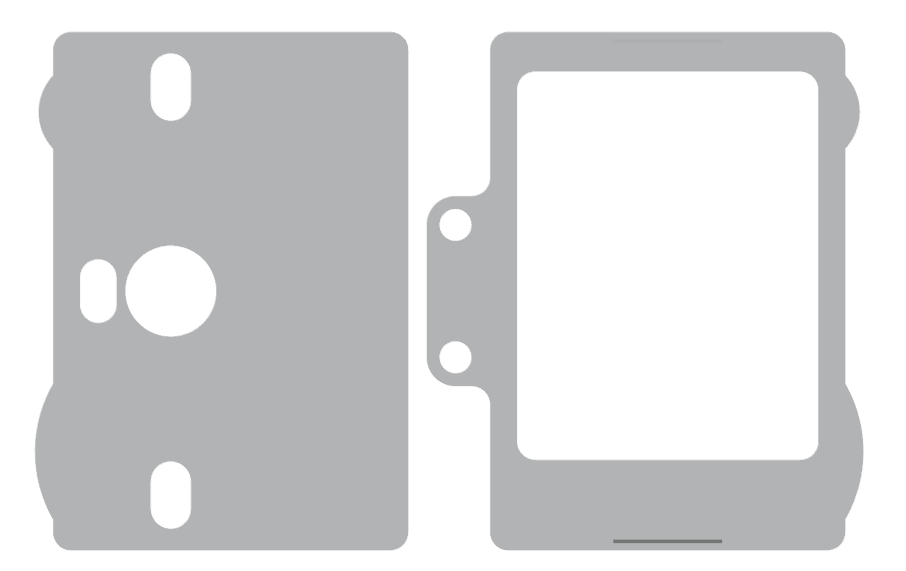
\includegraphics[width=\linewidth]{images/modelos3d/carcasa-husky-superior.png}
        \caption{Vista superior}
    \end{subfigure}
    \hfill
    \begin{subfigure}{0.4\textwidth}
        \centering
        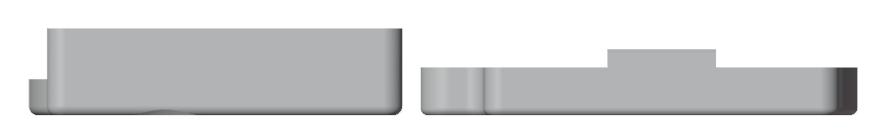
\includegraphics[width=\linewidth]{images/modelos3d/carcasa-husky-lateral.png}
        \caption{Vista Lateral}
    \end{subfigure}

    % -------- Segunda fila --------
    \begin{subfigure}{0.5\textwidth}
        \centering
        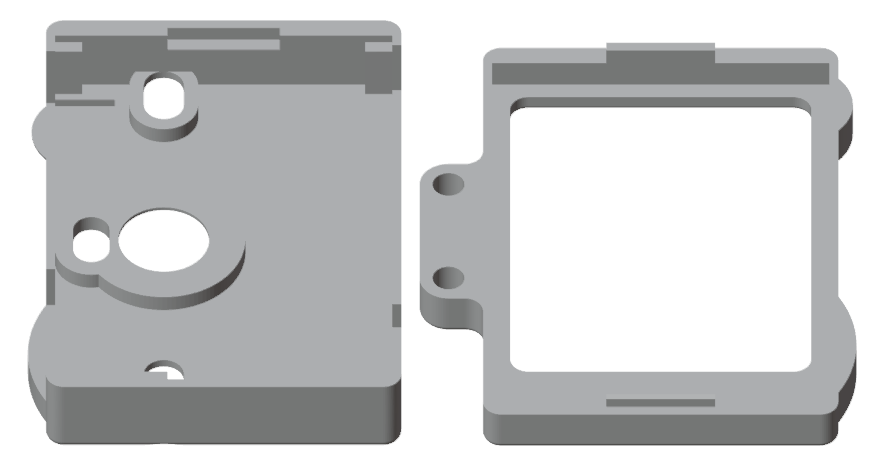
\includegraphics[width=\linewidth]{images/modelos3d/carcasa-husky-3d.png}
        \caption{Vista en perspectiva}
    \end{subfigure}

    \caption{Vistas del modelo tridimensional de la carcasa original de HuskyLens.}
    \label{fig:carcasa-husky-original}
\end{figure}

\FloatBarrier 

\subsection{Diseño conceptual}
% estructura general, criterios de decisión, integración con el robot

Con estos dos modelos como base para el diseño, se buscó fusionarlos en un solo modelo que permita agregar la cámara HuskyLens a su interior, manteniéndola fija en un ángulo determinado y de fácil acceso en caso de tener que configurarla o desarmar la estructura. Tomando como base las pruebas realizadas previas al rediseño de la carcasa, se definió el ángulo de inclinación de la cámara 16.5 grados con respecto al eje horizontal, que permite una visión cercana a Robotito, facilitando su funcionamiento, y que además logra mantener una coherencia estética y estructural con el modelo original, ya que un ángulo significativamente grande representa una pieza sobresaliente a la parte superior del robot que puede ser fácilmente rota al ser manipulada en un entorno educativo infantil.

\subsection{Proceso de modelado CAD}
% herramienta utilizada y metodología básica

La herramienta utilizada para el modelado tridimensional de la nueva carcasa fue Blender \cite{Blender} en su versión para el sistema operativo Windows. Con esta herramienta se logró importar los archivos de extensión .stl (Stereolithography) de cada modelo y trabajar sobre las superficies geométricas definidas en cada uno.

El primer paso para realizar el rediseño luego de obtenidos los dos modelos individuales de carcasa de Robotito y de cámara HuskyLens, fue ubicar a ambos en sus posiciones correspondientes al modelo objetivo. Para esto se ubica la carcasa de Robotito con el centro de su base en el origen (X=0, Y=0, Z=0) y luego se ubica el modelo de soporte de la cámara en la posición definida según las pruebas realizadas (ligeramente arriba de la parte superior de la carcasa de Robotito, sobre el borde del mismo, ubicando la zona correspondiente al lente de la cámara hacia la dirección ``frontal'' del robot, que además coincide con las ruedas frontales de Robotito, apuntando hacia ``abajo'' con una leve inclinación de 16.5 grados con respecto al plano horizontal).

Una vez ubicados ambos modelos en las posiciones correctas, se implementa una tercera estructura que respresenta la ``unión'' física entre ambos. Para eso se busca mantener la coherencia estética del modelo, intentando no utilizar ángulos muy forzados y simplificando la geometría utilizada.

Con los tres modelos presentes y ubicados en sus posiciones finales, se realizan repetidas operaciones booleanas de Unión de Blender. Esto logra unir dos piezas seleccionadas en una sola, haciendo que el modelo consista de la menor cantidad de piezas necesarias. Luego de ejecutadas las uniones se llega a un modelo de dos piezas que incluye la carcasa original de Robotito con una base para HuskyLens, y una tapa para asegurar la cámara luego de ubicada en el robot.

Finalmente, para mejorar la estética del modelo y asegurar su funcionamiento seguro como aplicación en un entorno educativo infantil, se realizaron dos agujeros (en la herramienta Blender) en el modelo de la carcasa para permitir que todo el cableado de la cámara se ubique de forma interna a la estructura del robot. Cada agujero corresponde a una entrada física de cables que permite la cámara, con sus tamaños correspondientes.

\subsection{Resultados y mejoras futuras}
% qué se logró y qué quedaría para una siguiente iteración

El resultado obtenido se detalla a continuación, donde se puede observar el diseño terminado con ambas piezas (carcasa y tapa) ya ubicados en sus respectivos lugares \\

\begin{figure}[htbp]
    \centering

    % -------- Primera fila --------
    \begin{subfigure}{0.49\textwidth}
        \centering
        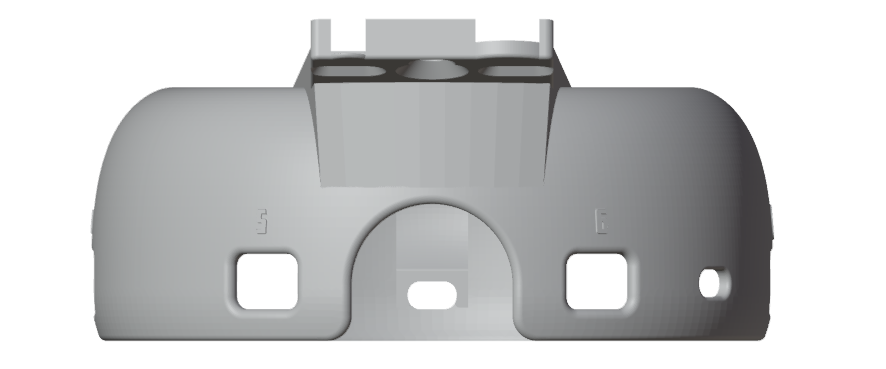
\includegraphics[width=\linewidth]{images/modelos3d/carcasa-nueva-frontal.png}
        \caption{Vista Frontal}
    \end{subfigure}
    \hfill
    \begin{subfigure}{0.49\textwidth}
        \centering
        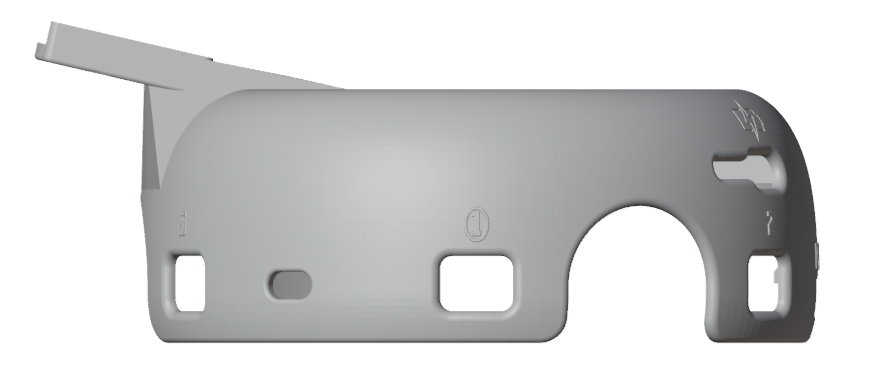
\includegraphics[width=\linewidth]{images/modelos3d/carcasa-nueva-lateral.png}
        \caption{Vista Lateral}
    \end{subfigure}

    % -------- Segunda fila --------
    \begin{subfigure}{0.49\textwidth}
        \centering
        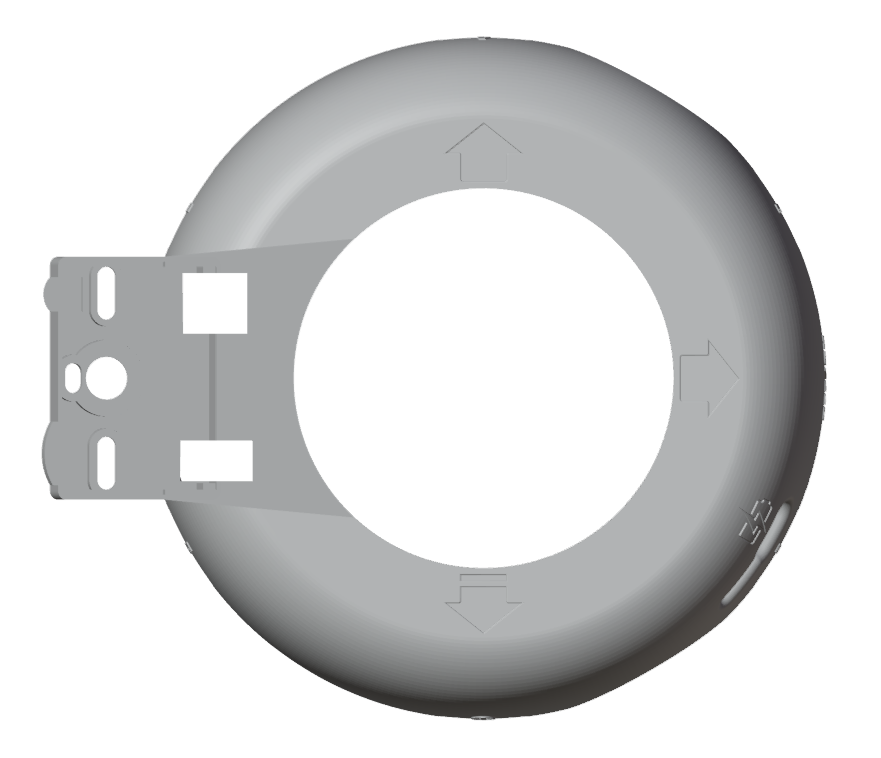
\includegraphics[width=\linewidth]{images/modelos3d/carcasa-nueva-superior.png}
        \caption{Vista Superior}
    \end{subfigure}
    \hfill
    \begin{subfigure}{0.49\textwidth}
        \centering
        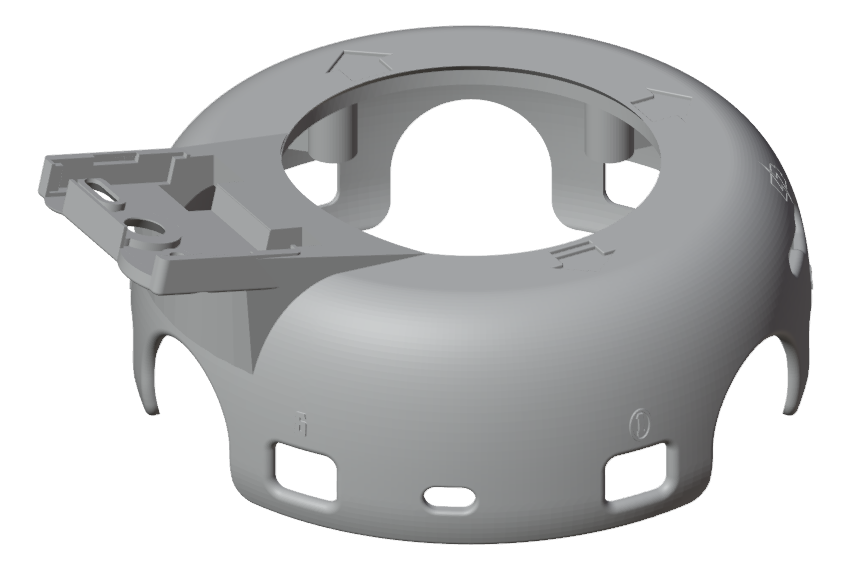
\includegraphics[width=\linewidth]{images/modelos3d/carcasa-nueva-3d.png}
        \caption{Vista en perspectiva}
    \end{subfigure}

    \caption{Vistas del modelo tridimensional de la carcasa nueva de Robotito con soporte para HuskyLens.}
    \label{fig:carcasa-husky-original}
\end{figure}

\FloatBarrier

Infelizmente no se pudo realizar la impresión del modelo por lo que este se mantiene conceptual. Resultaría interesante un rediseño del mismo para mejorar su aspecto estético y hacerlo más llamativo a un público objetivo infantil. A partir de esto se podría analizar si genera más interés en un formato de semejanza con lo ``cotidiano'', por ejemplo animales o vehículos, o quizás un formato más ``robótico'' que despierte curiosidad por su aspecto poco común.

\end{appendix}


%%%%%%%%%%%%%%%%%%%%%%%%%%%%%%%%%%%%%%%%%%%%%%%%%%%%%%%%%%%%%%%%%%%%%%%%%%%%%%%%%%%%%%%%%%%%%%%%

\end{document}
